\subsection{Local Map Generation}
\subsubsection{Overview}
The main question in this section is whether raw side scan sonar data can be transformed into stable local maps and reliable landmark measurements for later SLAM use. This is important because the SLAM back-end does not operate directly on raw sonar returns. It depends on the data-processing pipeline to produce geometrically consistent maps, extract repeatable landmarks, and assign measurements, uncertainties, and descriptors that are useful for data association and loop closure.
\\ \\
This section presents the results obtained from the local map generation stage of the pipeline. The evaluation covers swath processing, probabilistic local map generation, and feature extraction. Together, these stages progressively transform raw side scan sonar measurements into corrected swaths, spatially consistent reflectivity maps, and finally compact landmark representations suitable for SLAM.
\\ \\
The local map is an important intermediate representation, but it is not efficient to use the full dense map directly for repeated data association. As the mission grows, dense map comparison becomes increasingly expensive, and much of the image data contains background texture that is not useful for identifying repeatable landmarks. For this reason, the feature extraction stage compresses the useful map information into a sparse set of landmarks with associated measurements, uncertainties, descriptors, and probabilistic characteristics. These landmarks form a compact feature database that can be searched much faster than the full reflectivity map when proposing candidate matches or loop closures.
\\ \\
The local map generation results are used to evaluate both the quality of the produced map data and the cost of producing it. The first part of the evaluation follows the data through the processing chain and checks whether each stage produces the expected output, corrected swaths after geometric correction and blind zone removal, meaningful candidate support after pruning, stable local reflectivity maps after accumulation and normalization, and repeatable landmark detections after feature extraction. These qualitative results show whether the output is suitable for later SLAM use.
\\ \\
The second part evaluates the computational cost of the individual local map generation stages. Runtime, CPU usage, and memory consumption are measured for swath processing, map generation, and feature extraction separately. These measurements are not meant to replace the complete pipeline schedulability analysis later in the chapter, but to show where the main isolated costs come from and how different parameters affect each stage.
\\ \\
For the swath processing stage, the results focus on geometric correction, blind zone removal, intensity normalization, and runtime behavior. For the map generation stage, the results focus on probabilistic pruning, persistent map state construction, normalized local map reconstruction, fast gap filling, and computational cost. For the feature extraction stage, the results focus on landmark segmentation, descriptor generation, landmark measurement quality, optional height estimation, and the runtime impact of these operations.
\\ \\
It is important to note that map generation and feature extraction depend strongly on the quality of the underlying state estimate. When aiding measurements are available, the local maps are expected to remain spatially consistent and visually coherent, which also improves landmark stability. During dead reckoning periods, accumulated estimator drift can gradually degrade map quality and reduce the reliability of extracted features. The following subsections therefore evaluate not only the individual algorithms, but also whether their combined output is accurate, useful for SLAM, and practical for real-time embedded deployment.



\newpage



\subsubsection{Parameters}
The main tuning parameters used in the local map generation experiments are summarized in Table \ref{tab:local-map-generation-parameters}. Only the parameters most relevant to the behavior, quality, and computational cost of the implemented methods are included here. Configuration values related mainly to sensor mounting geometry, ROS2 communication, frame alignment, or programmer facing implementation details are omitted, since they are less important for interpreting the algorithmic results.
\begin{table}[H]
    \centering
    \caption{Main parameters used in the local map generation experiments.}
    \label{tab:local-map-generation-parameters}
    \begin{tabular}{l l}
        \hline
        Parameter & Value \\
        \hline

        \multicolumn{2}{l}{\textbf{Swath processing}} \\
        Illumination EMA period & 200 \\
        Port blind zone scale & 0.45 \\
        Starboard blind zone scale & 0.35 \\
        \\[-0.6em]

        \multicolumn{2}{l}{\textbf{Map generation}} \\
        Dense map update interval & 100 swaths \\
        Maximum map update gap & 5.0 s \\
        Map resolution & 0.03 m/pixel \\
        Chunk size & 64 pixels \\
        Maximum chunk age & 2 \\
        Approximate pruning threshold $\varepsilon_{\mathrm{approx}}$ & 0.96850 \\
        Probabilistic pruning threshold $\varepsilon_{\mathrm{prob}}$ & 0.00187 \\
        Minimum fill neighbors & 3 \\
        Maximum fill passes & 5 \\
        \\[-0.6em]

        \multicolumn{2}{l}{\textbf{Feature extraction}} \\
        Bilateral filter diameter & 31 pixels \\
        Bilateral filter $\sigma_{\mathrm{color}}$ & 80.0 \\
        Bilateral filter $\sigma_{\mathrm{space}}$ & 100.0 \\
        Semantic local window size & 51 pixels \\
        Semantic local offset & 3.3 \\
        Semantic support search radius & 21 pixels \\
        Minimum semantic support & 100 pixels \\
        Minimum landmark area & 5000 pixels \\
        Base range uncertainty $\sigma_r$ & 0.030 m \\
        Base bearing uncertainty $\sigma_\theta$ & 0.400 deg \\
        Range uncertainty scale $\alpha_r$ & 0.025 \\
        Bearing uncertainty scale $\alpha_\theta$ & 0.005 \\

        \hline
    \end{tabular}
\end{table}
\noindent
The swath processing parameters consist of the illumination EMA period and the channel dependent blind zone scale factors. The EMA period controls how slowly the estimated illumination envelope is allowed to vary during intensity normalization, while the blind zone scale factors determine how aggressively the near nadir region is removed for the port and starboard channels. These values were tuned empirically to obtain a reasonable separation between the water column and the first valid seabed returns in the measured sonar data.
\\ \\
The map generation parameters control both map quality and computational cost. The dense map update interval and maximum update gap determine how often the dense local map is rebuilt and published. The map resolution sets the final spatial sampling of the generated map and is one of the most important parameters for both runtime and memory usage. The chunk size and maximum chunk age control the sparse chunked map representation, affecting how long old map regions are retained and how large the active map becomes in practice.
\\ \\
The two pruning thresholds, $\varepsilon_{\mathrm{approx}}$ and $\varepsilon_{\mathrm{prob}}$, govern how aggressively low contribution candidate cells are removed during the approximate and probabilistic pruning stages. These parameters strongly influence the tradeoff between retained map detail and computational efficiency. The gap filling parameters determine how aggressively small holes in the normalized local map are repaired, where the minimum number of valid neighbors controls how conservative the fill operation is and the number of fill passes determines how many times the local repair step is allowed to propagate.
\\ \\
The feature extraction parameters control the filtering, semantic segmentation, and final pruning of candidate landmarks. The bilateral filter parameters determine how strongly speckle noise is suppressed while preserving echo and shadow boundaries. The semantic segmentation parameters define the local intensity window, the threshold offset used to detect bright and dark candidates, and the support requirement between nearby echo and shadow regions. The minimum landmark area is used as a final size based pruning step after segmentation and labeling. This removes very small regions that are more likely to be noise, fragmented artifacts, or unstable segmentation leftovers than useful landmarks. This is especially important because the semantic method is designed to be general and robust for medium to large acoustic structures, but very small detections can still be unreliable. It is therefore safer to reject weak small candidates early than to pass unstable landmarks into data association, where incorrect matches are harder to correct later.
\\ \\
The landmark measurement uncertainty parameters define how much confidence is assigned to extracted landmark measurements. The base range and bearing uncertainties describe the nominal measurement noise, while the range dependent scaling factors increase the uncertainty for farther landmarks. This reflects the fact that distant features are generally less reliable due to lower resolution, weaker acoustic return, beam spreading, and larger sensitivity to pose and map errors.
\\ \\
Additional parameters exist in the implementation, including detailed sonar mounting geometry, transducer beam configuration, frame alignment offsets, and height estimation settings. These are important for the full software system, but are omitted from this summary to keep the results section focused on the parameters that most directly affect local map quality, feature extraction behavior, and computational performance.



\newpage



\subsubsection{Swath Processing}
\paragraph{Geometric correction} \mbox{}\\[0.5em] \noindent
The swath processing stage was evaluated by inspecting the intermediate outputs produced after geometric correction, blind zone removal, and intensity normalization. These results show how the raw sonar measurements are progressively transformed into a cleaner and more consistent swath representation suitable for later map generation.
\begin{figure}[H]
    \centering
    \includegraphics[width=0.95\linewidth]{Pictures/Results/Local_Map_Generation/Swath_Processing/Geometric_correction_zoomed_out.png}
    
    \vspace{0.5em}
    
    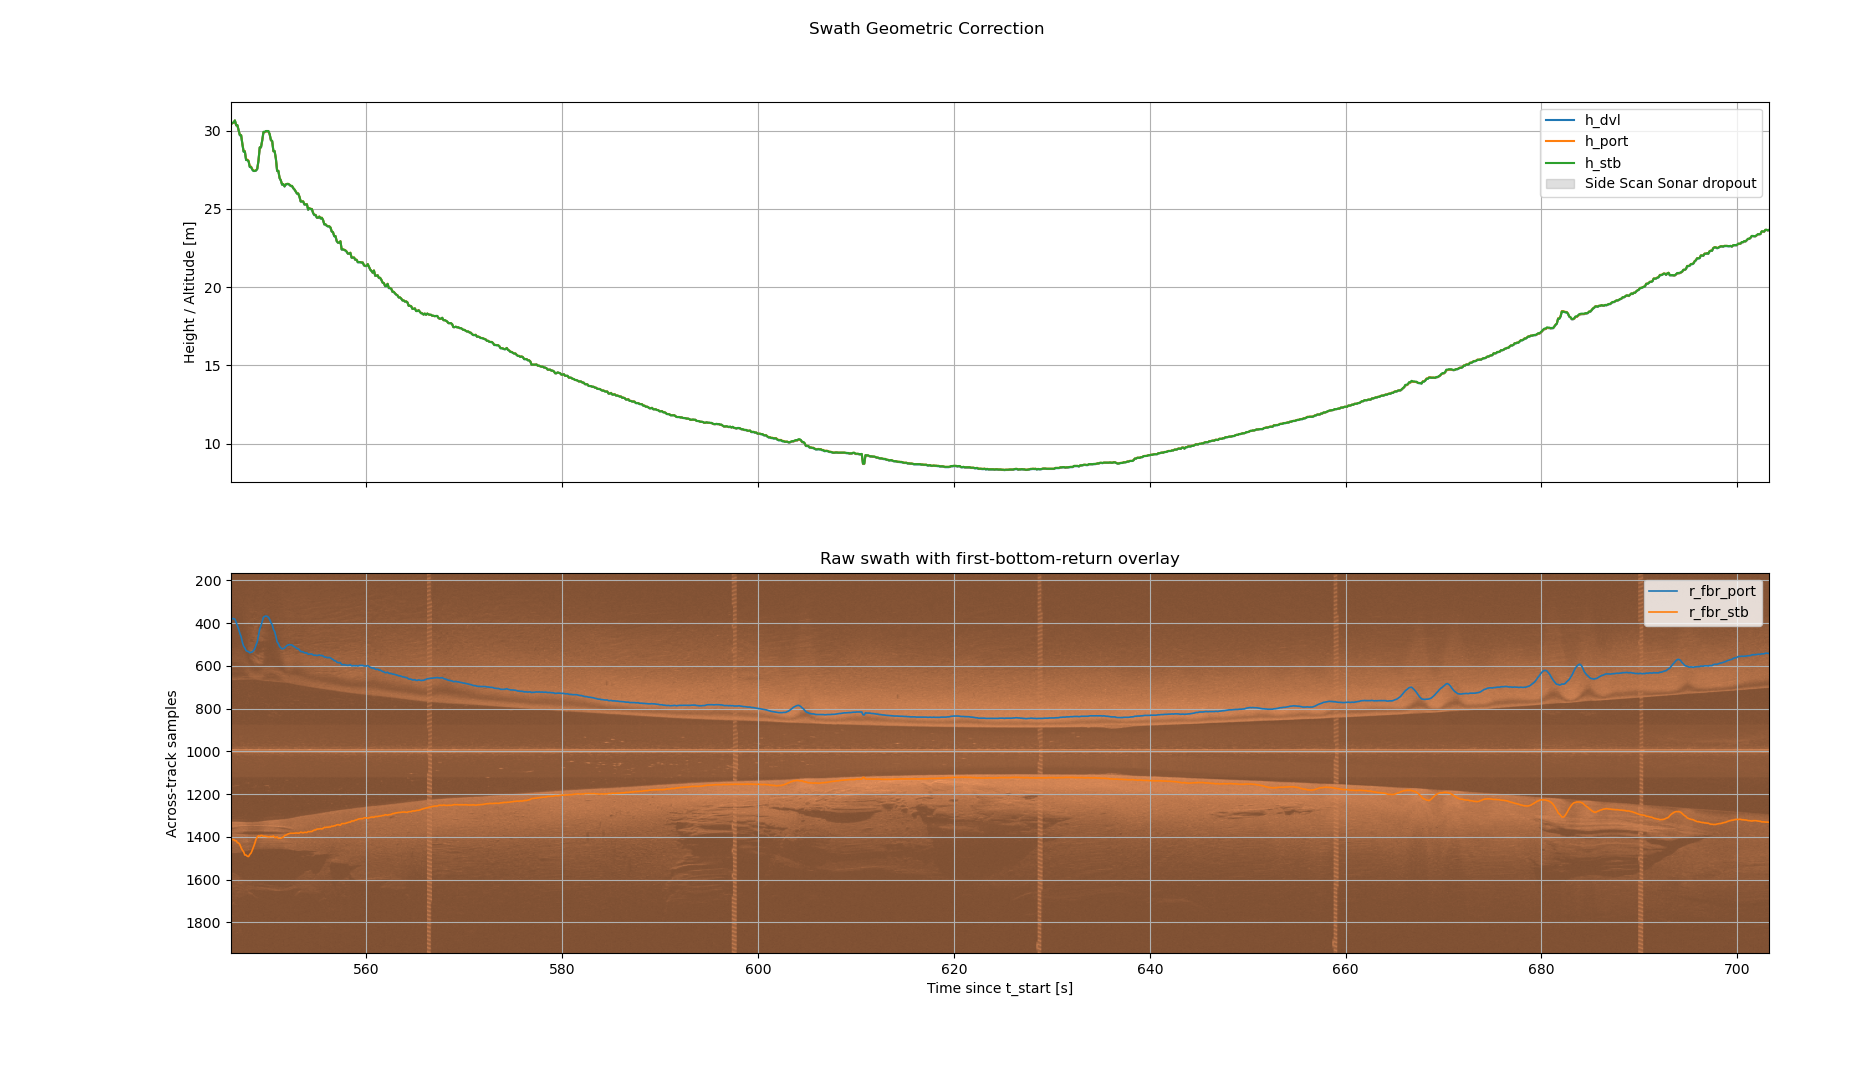
\includegraphics[width=0.95\linewidth]{Pictures/Results/Local_Map_Generation/Swath_Processing/Geometric_correction_zoomed_in.png}
    \caption{Geometric correction result shown at two spatial scales. The upper image shows the full mission view of the estimated first bottom return boundary, while the lower image shows a zoomed in view of the same result. In both cases, the corrected boundary follows the expected seabed intersection geometry and separates the near nadir water column region from the valid seabed returns. Note that $h_{\mathrm{dvl}}$, $h_{\mathrm{port}}$, and $h_{\mathrm{stb}}$ are nearly identical, with a maximum difference of only about $0.2\,\mathrm{m}$. As a result, the three height curves largely overlap and visually appear as a single line, even though they represent three separate estimates.}
    \label{fig:results-local-map-generation-swath-processing-geometric-correction}
\end{figure}

\newpage

\noindent
These figures illustrate the geometric correction stage used before blind zone removal. The estimated transducer height and beam geometry provide a physically motivated first return boundary for each channel, which is then used to identify the portion of the swath that can correspond to valid seabed returns.
\\ \\
In practice, the blind zone boundary required an additional empirical scaling factor to match the observed sonar data well. Ideally, the purely geometric model should have been sufficient on its own, but without this correction the predicted boundary removed too much of the valid seabed region. A similar need for practical blind zone correction was also observed in Haraldstads earlier master thesis \cite{side_scan_sonar_master_thesis}, although the underlying cause was not fully resolved there either.  
\\ \\
The main observation in the present results is that this mismatch appears to be close to constant over time, which is why a fixed scaling factor works reasonably well in practice. At the same time, the zoomed in result shows that the error is not perfectly constant. In some parts of the swath the blind zone is removed almost exactly as desired, while in other parts slightly too much valid seabed is removed. This indicates that the remaining mismatch is not purely geometric, but instead contains an additional varying component. The most likely explanation is that the first physically possible seabed return predicted by the geometric model does not perfectly coincide with the first strong measured backscatter in the real sonar image. This varying error may stem from unmodeled timing effects, uncertainties in the effective beam geometry, mounting inaccuracies, sonar specific signal formation, or differences between the instant of transmission, the instant of reception, and the time associated with the external aiding data. It is therefore reasonable that the required correction differs slightly between the port and starboard channels.

\newpage

\paragraph{Processing} \mbox{}\\[0.01em] \noindent
\begin{figure}[H]
    \centering
    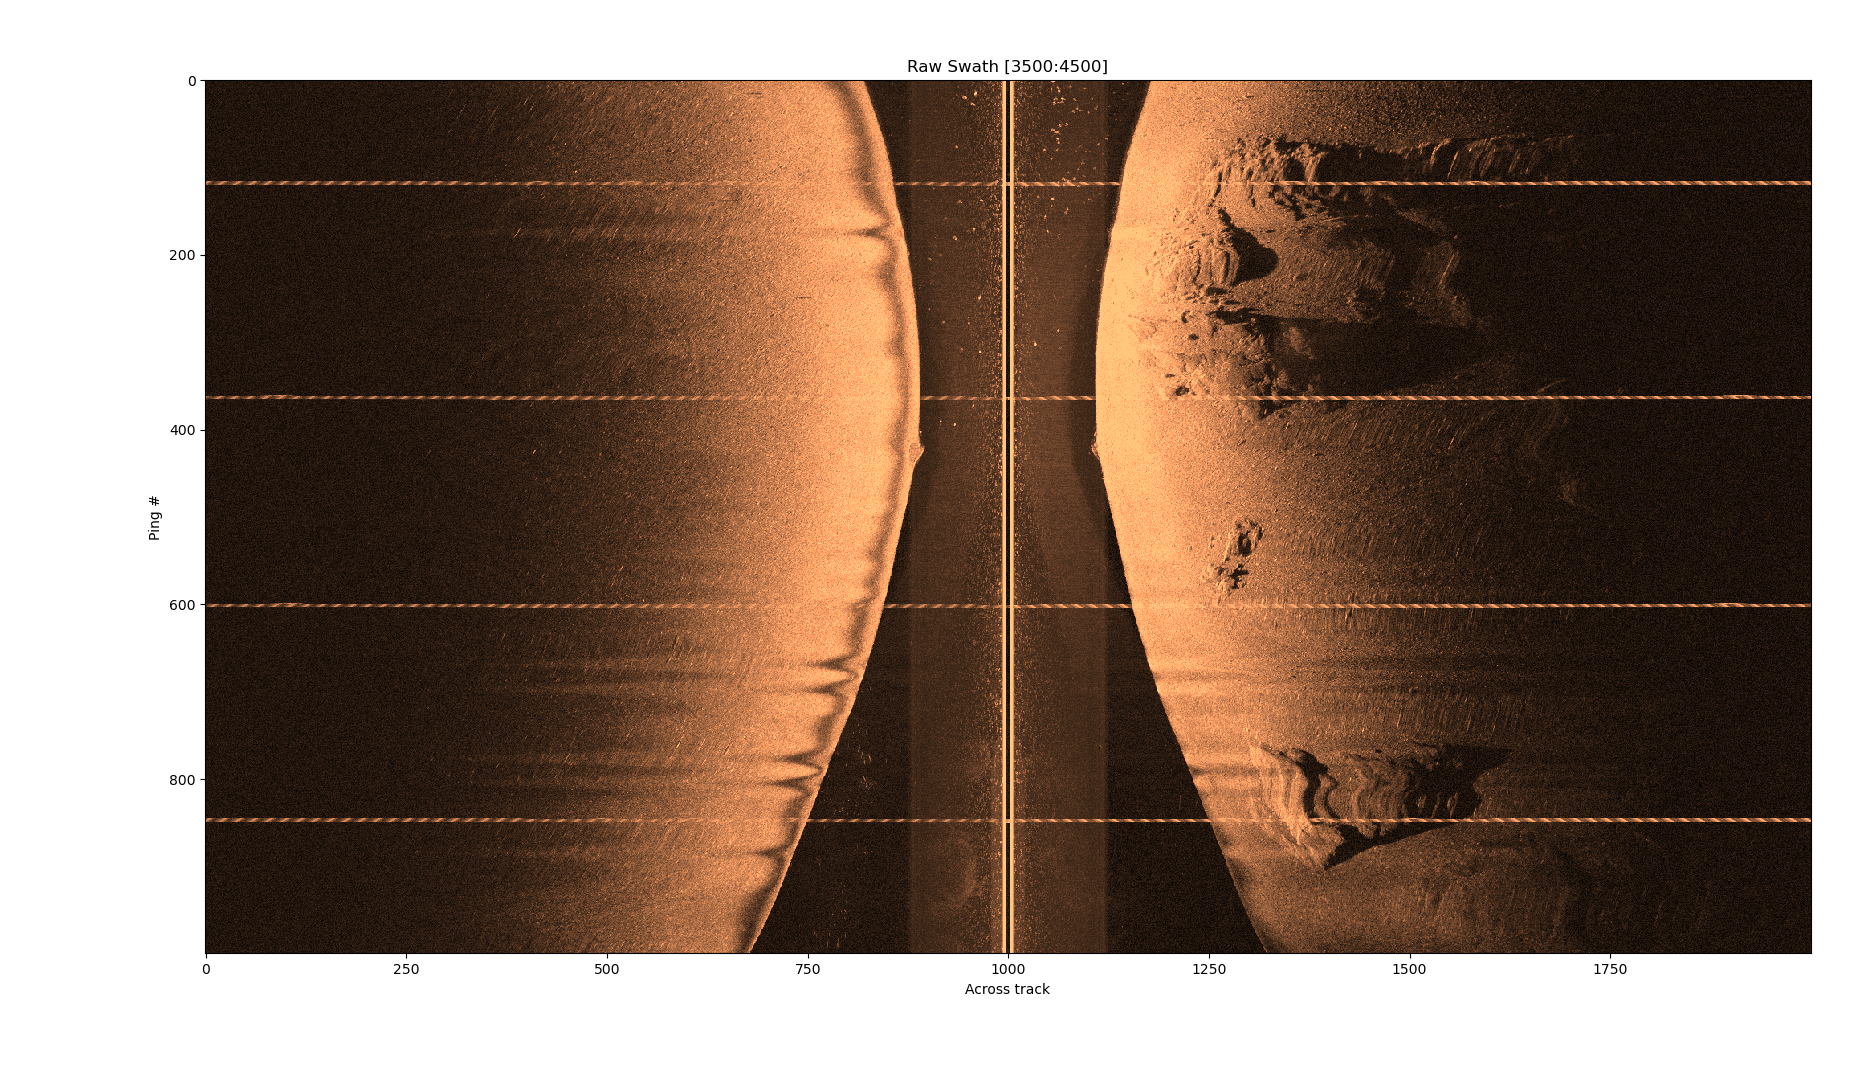
\includegraphics[width=0.7\linewidth]{Pictures/Results/Local_Map_Generation/Swath_Processing/Raw.png}
    
    \vspace{0.01em}
    
    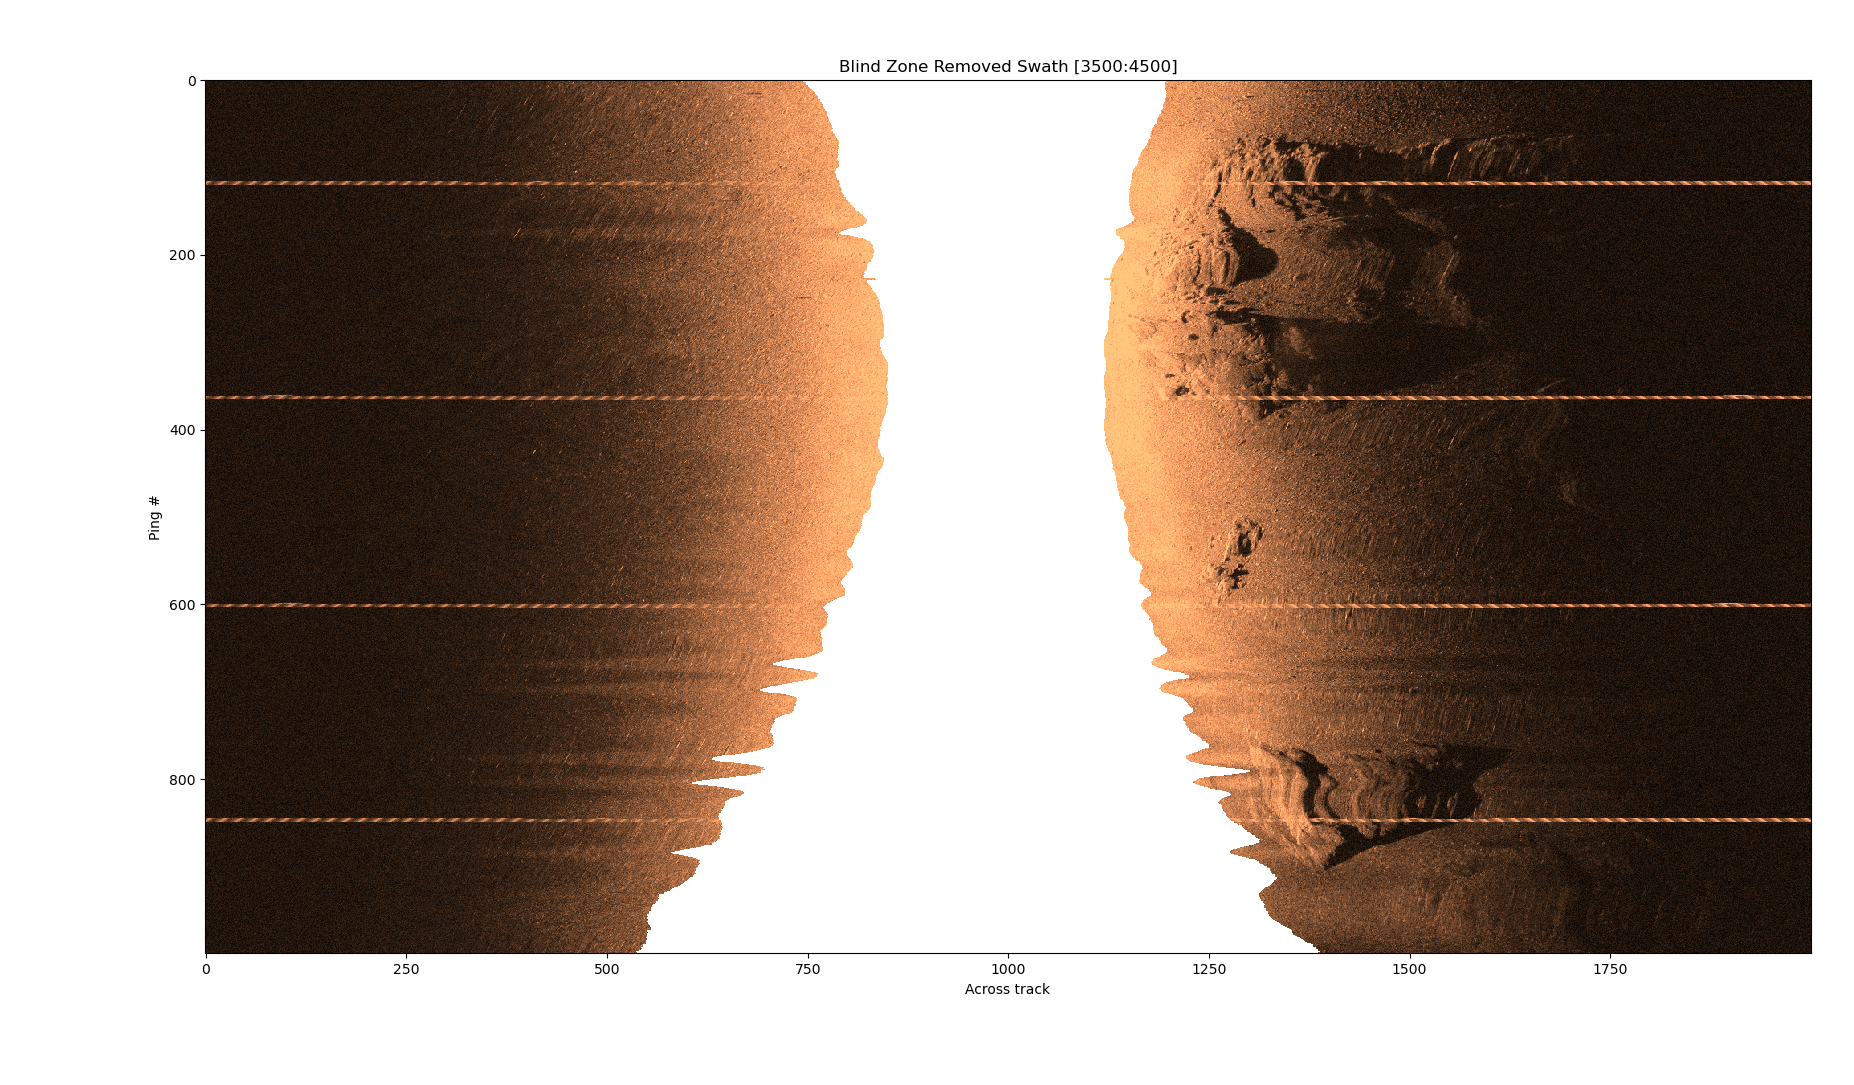
\includegraphics[width=0.7\linewidth]{Pictures/Results/Local_Map_Generation/Swath_Processing/Blind_Zone_Removed.png}
    
    \vspace{0.01em}
    
    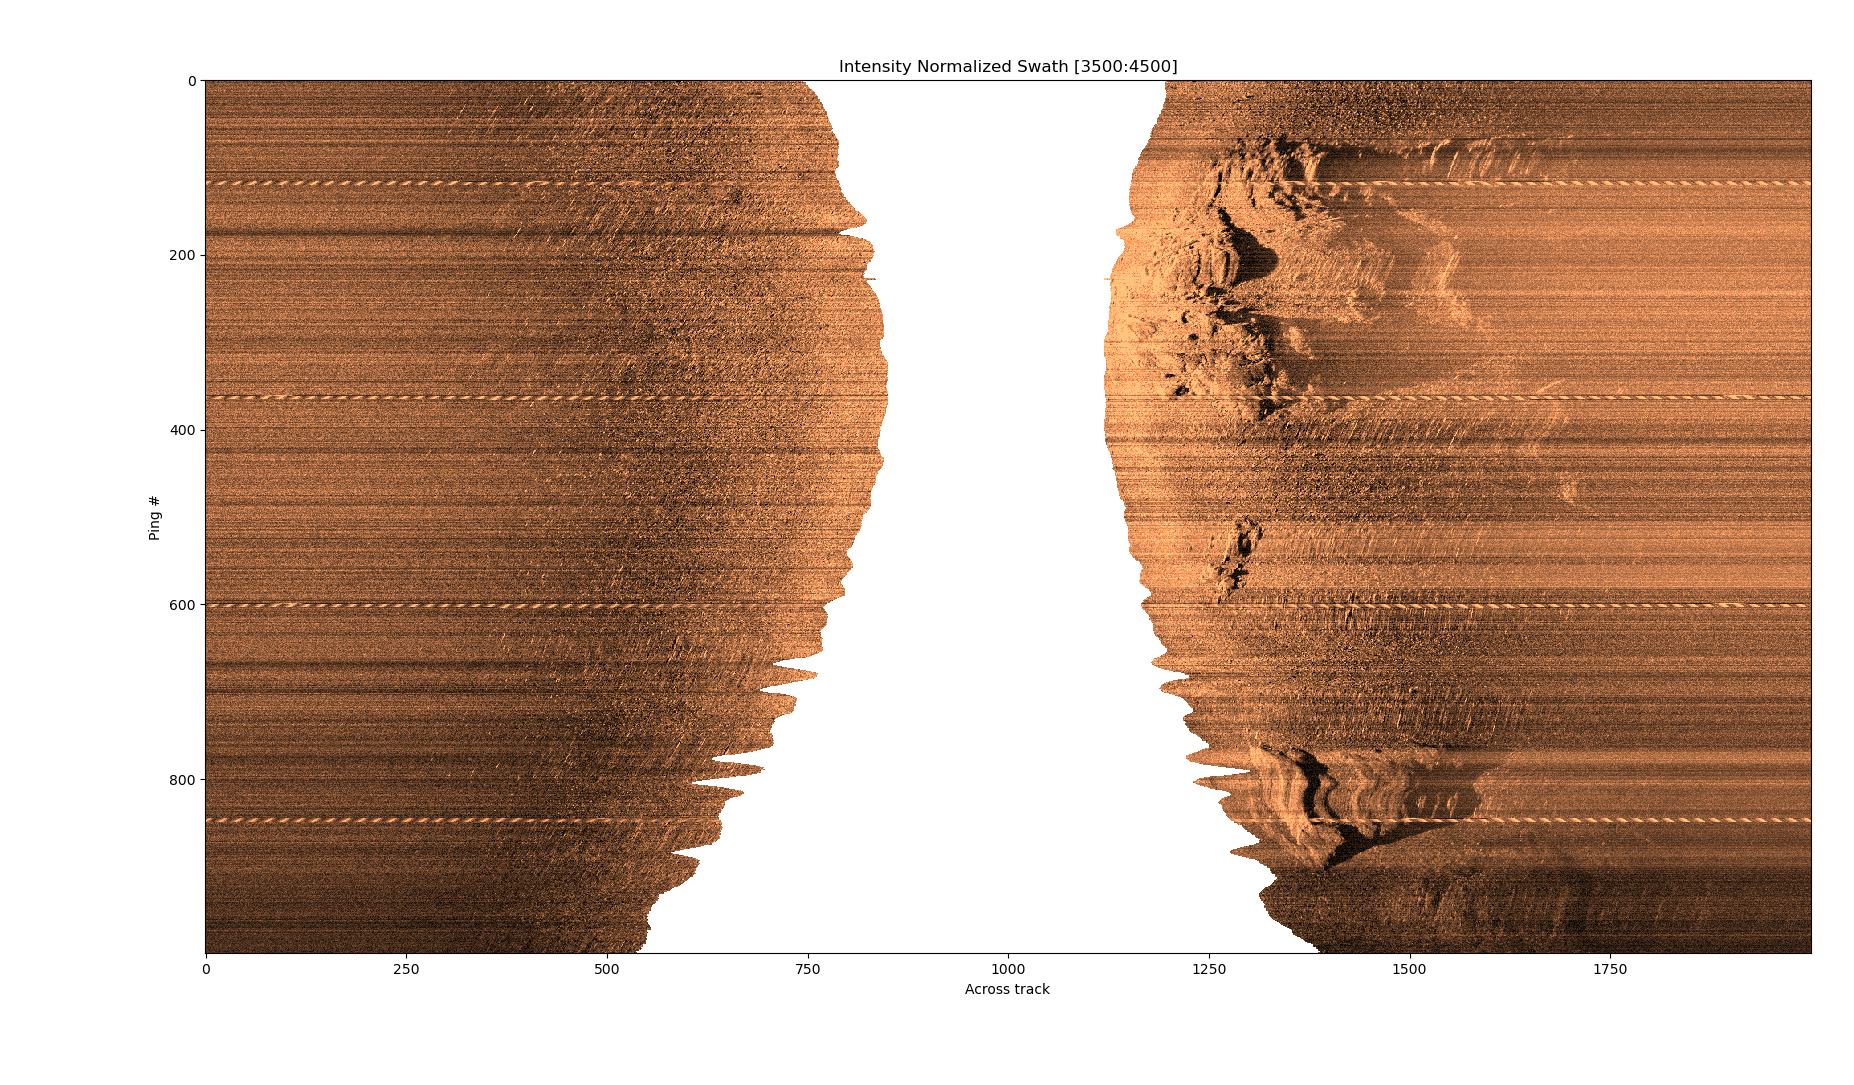
\includegraphics[width=0.7\linewidth]{Pictures/Results/Local_Map_Generation/Swath_Processing/Intensity_Normalized.png}
    \caption{Swath processing result shown at three stages of the pipeline zoomed in on a specific period in time. The top image shows the raw swath data before processing. The middle image shows the same swaths after blind zone removal, where the near nadir water column region has been masked out. The bottom image shows the final result after intensity normalization using the EMA based illumination estimate, where the large scale brightness variation is reduced and the relative seabed texture becomes clearer.}
    \label{fig:results-local-map-generation-swath-processing-pipeline}
\end{figure}

\newpage

\noindent
These figures show the main stages of the swath processing pipeline. The top image shows the raw swath received directly from the sonar. The middle image shows the result after blind zone removal using the corrected first return boundary together with the empirically tuned blind zone scaling discussed above. The bottom image shows the final output after intensity normalization, where the slowly varying illumination trend across the swath has been reduced.
\\ \\
The effect of the normalization is clearly visible, as the large scale range dependent brightness variation is reduced and the relative seabed structure becomes easier to interpret. Although the illumination is not perfectly uniform across all swaths, the overall result is stable and visually consistent. This is especially important because the normalized output obtained here is very similar to the result achieved with the cubic smoothing spline method used in Haraldstads thesis \cite{side_scan_sonar_master_thesis}, shown in Figure \ref{fig:results-local-map-generation-swath-processing-cubic-spline}. The main difference is therefore not primarily in the visual result, but in the computational cost. While the spline based approach can produce similarly good normalization, it is too computationally expensive for real time execution on embedded systems. The EMA based approach used here therefore provides a practical compromise, achieving nearly the same qualitative result while remaining lightweight enough for onboard real time swath processing.

\begin{figure}[H]
    \centering
    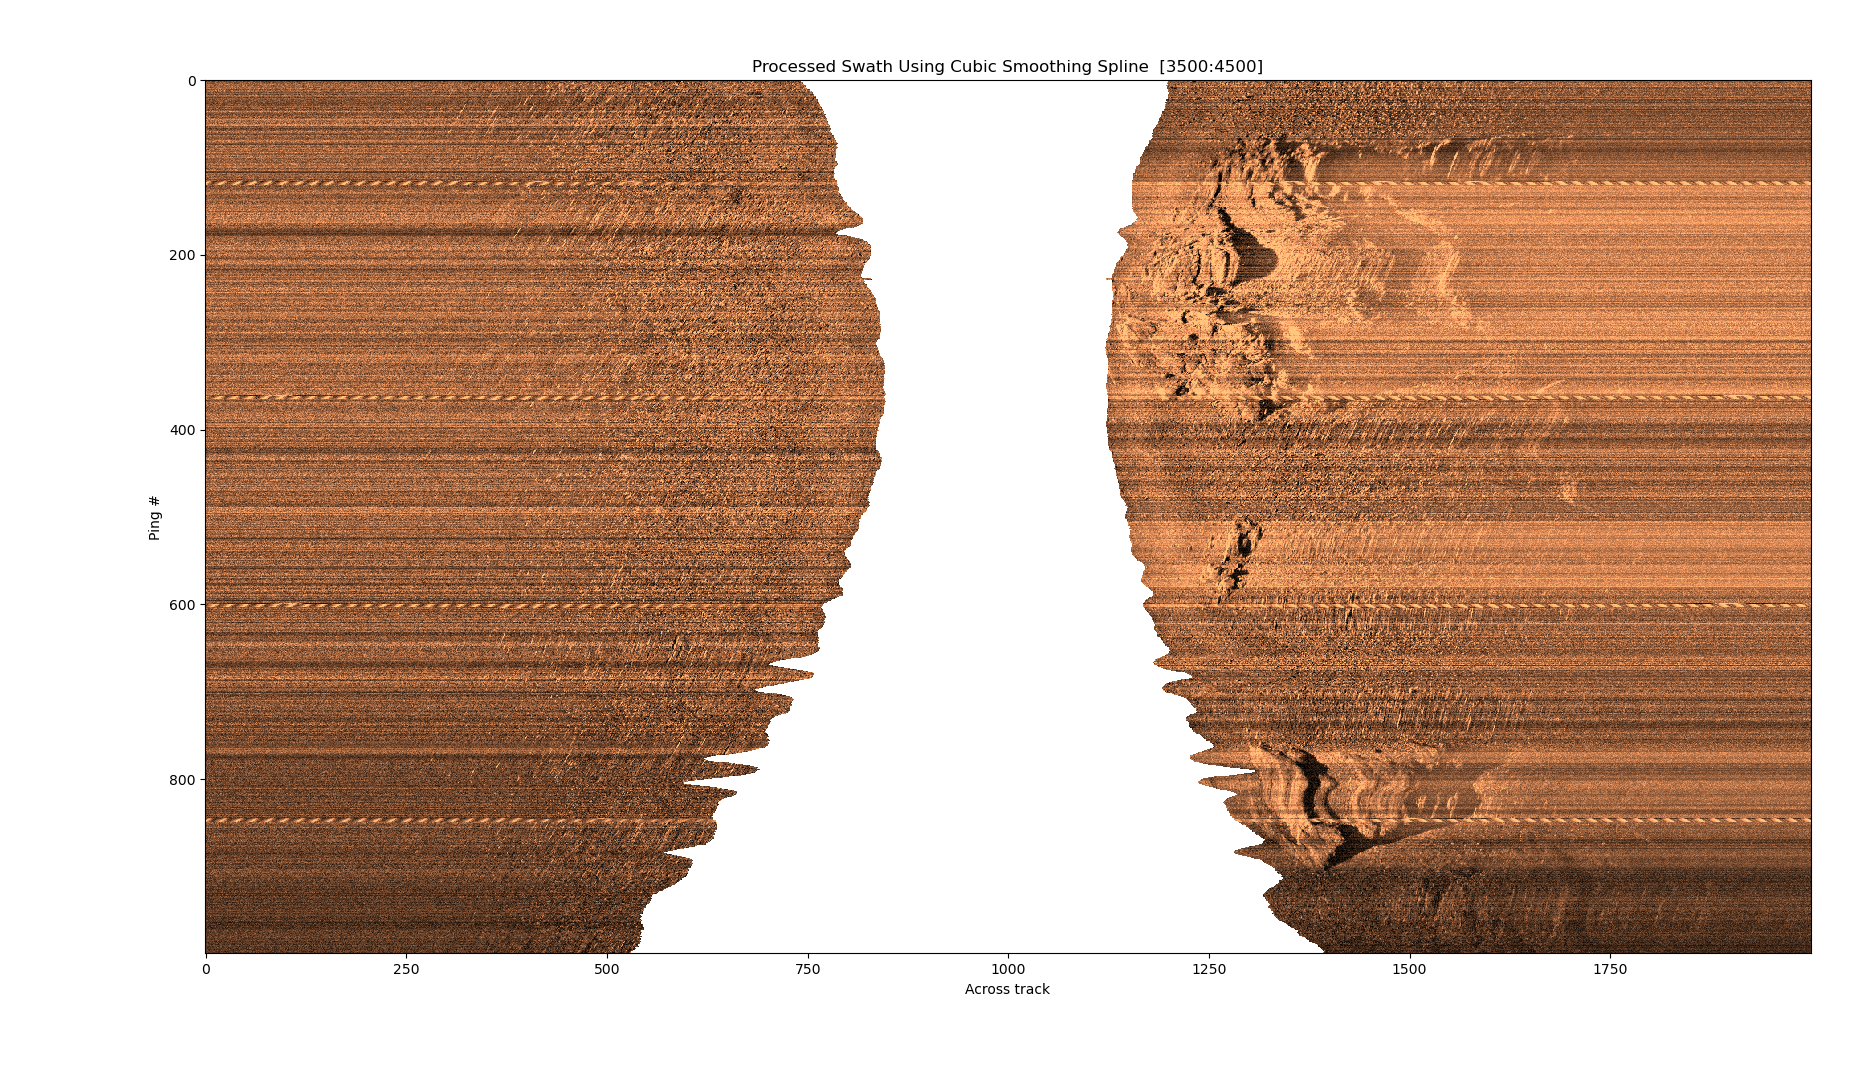
\includegraphics[width=1.0\linewidth]{Pictures/Results/Local_Map_Generation/Swath_Processing/Cubic_Smoothing_Spline.png}
    \caption{Normalization result obtained using the cubic smoothing spline based method from Haraldstads thesis \cite{side_scan_sonar_master_thesis}. The visual result is very similar to the EMA based normalization used in this work, but the spline based approach is significantly more computationally expensive and is therefore not suitable for real time embedded operation.}
    \label{fig:results-local-map-generation-swath-processing-cubic-spline}
\end{figure}

\newpage

\paragraph{Performance} \mbox{}\\[0.5em] \noindent
\begin{figure}[H]
    \centering
    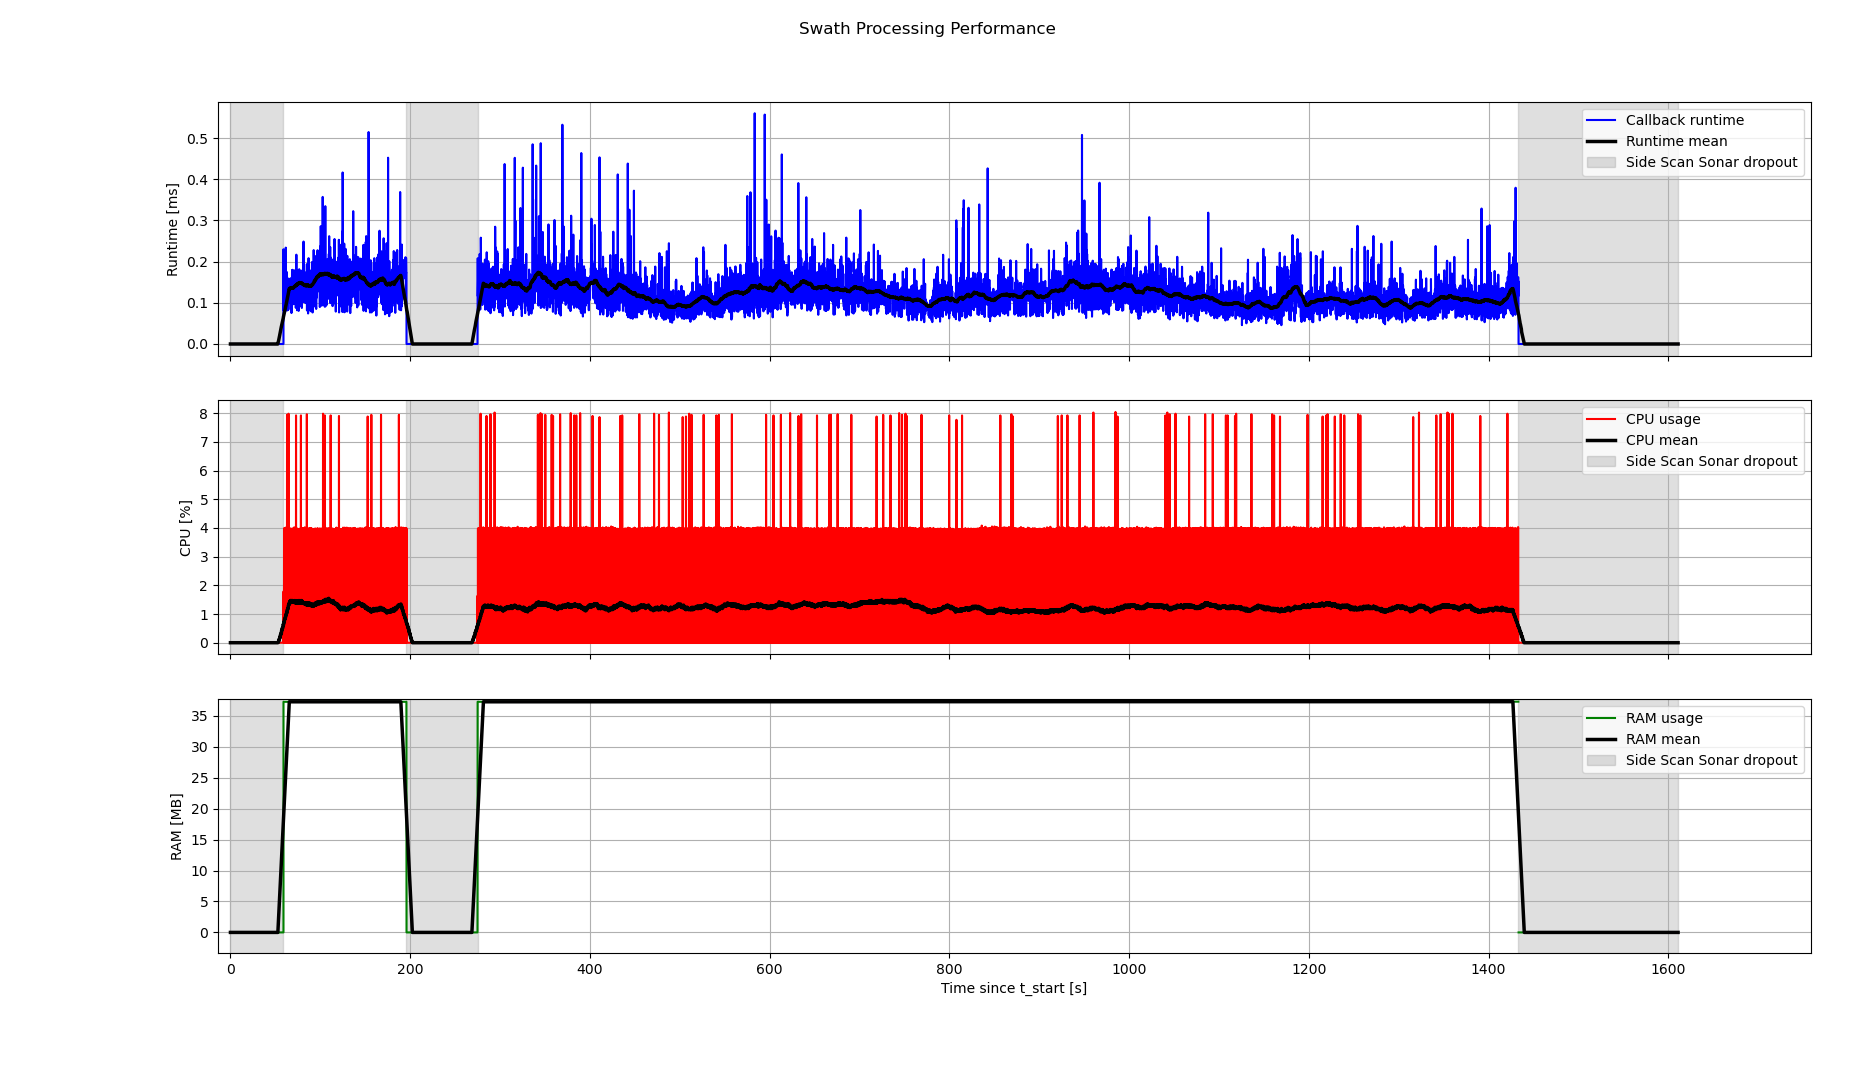
\includegraphics[width=1.0\linewidth]{Pictures/Results/Local_Map_Generation/Swath_Processing/Performance.png}
    \caption{Runtime, CPU usage, and memory consumption of the swath processor during operation.}
    \label{fig:results-local-map-generation-swath-processing-performance}
\end{figure}
\noindent
The computational performance of the swath processing stage was evaluated by measuring runtime, CPU usage, and memory consumption during execution. The runtime remains low enough for real time operation, which was one of the primary motivations for replacing the earlier spline based normalization approach with the present EMA based method.
\\ \\
Compared with a more computationally expensive smoothing based illumination estimate, the EMA based normalization significantly reduces the processing cost while still producing a sufficiently good illumination correction for the present task. CPU usage remains modest, and most of the observed memory footprint is dominated by the ROS2 execution environment rather than by the swath processing algorithm itself. These results indicate that the implemented swath processor is computationally lightweight and suitable for integration into the complete SLAM pipeline.



\newpage



\subsubsection{Map Generation}
\paragraph{Pruning stage} \mbox{}\\[0.5em] \noindent
\begin{figure}[H]
    \centering
    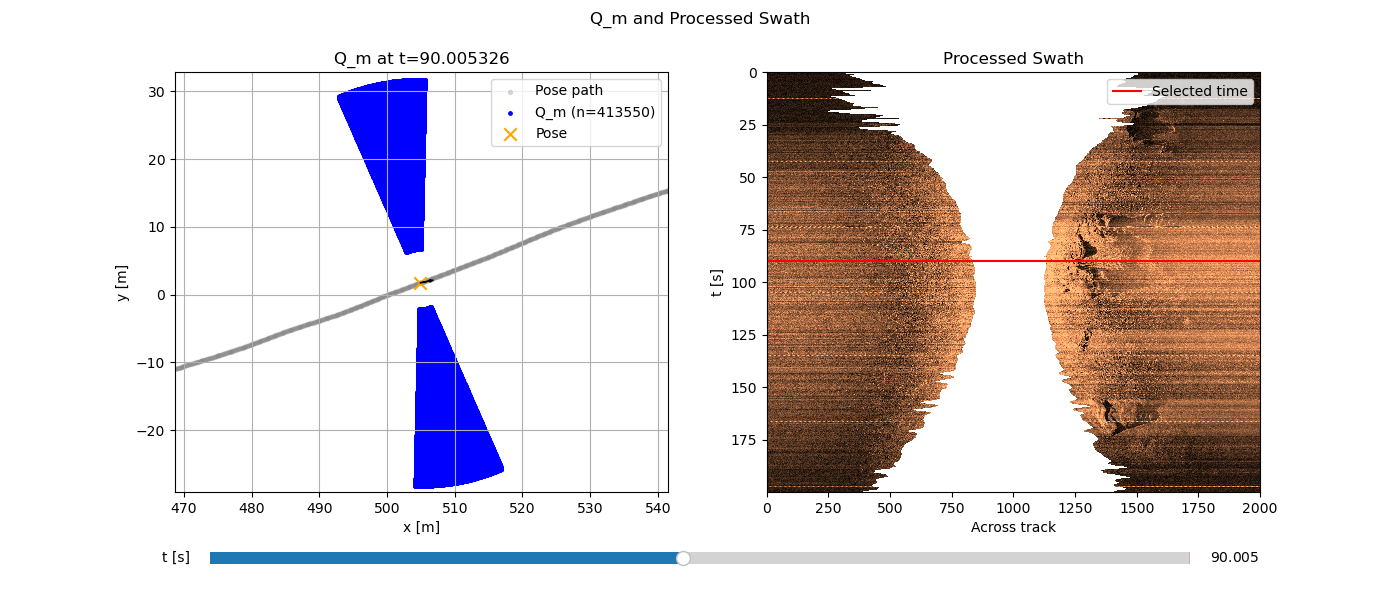
\includegraphics[width=0.93\linewidth]{Pictures/Results/Local_Map_Generation/Map_Generation/Q_m_pruned_1_zoomed_out.png}
    
    \vspace{0.01em}
    
    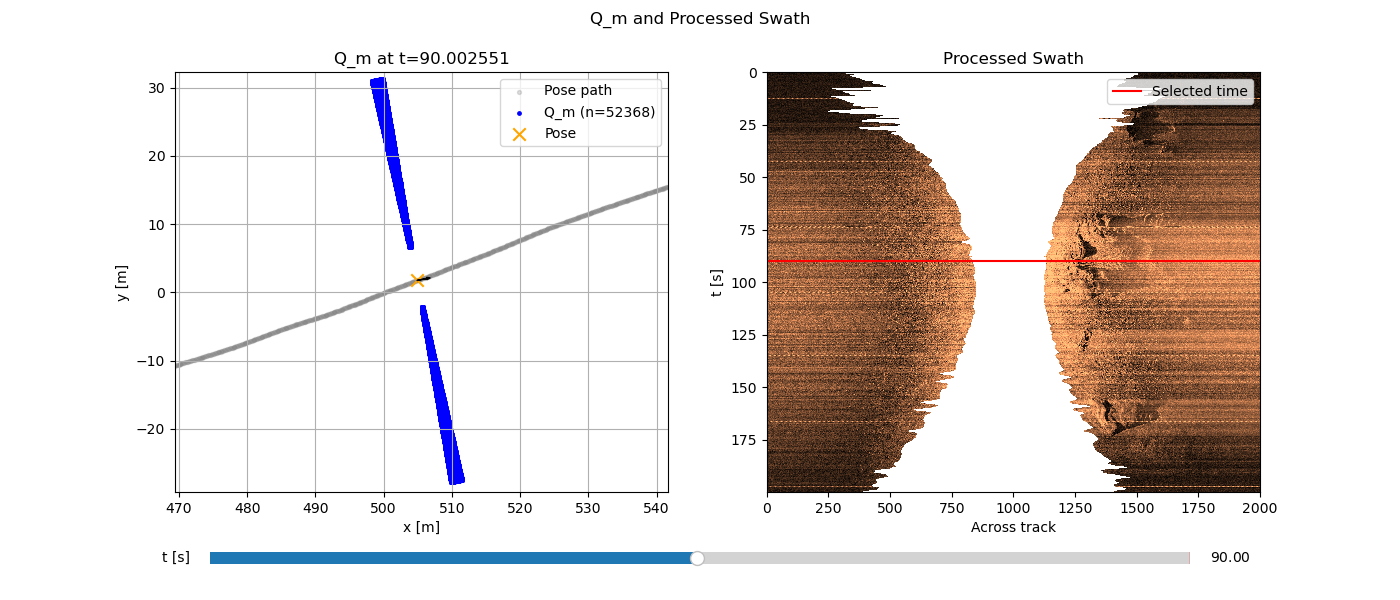
\includegraphics[width=0.93\linewidth]{Pictures/Results/Local_Map_Generation/Map_Generation/Q_m_pruned_2_zoomed_out.png}
    
    \vspace{0.01em}
    
    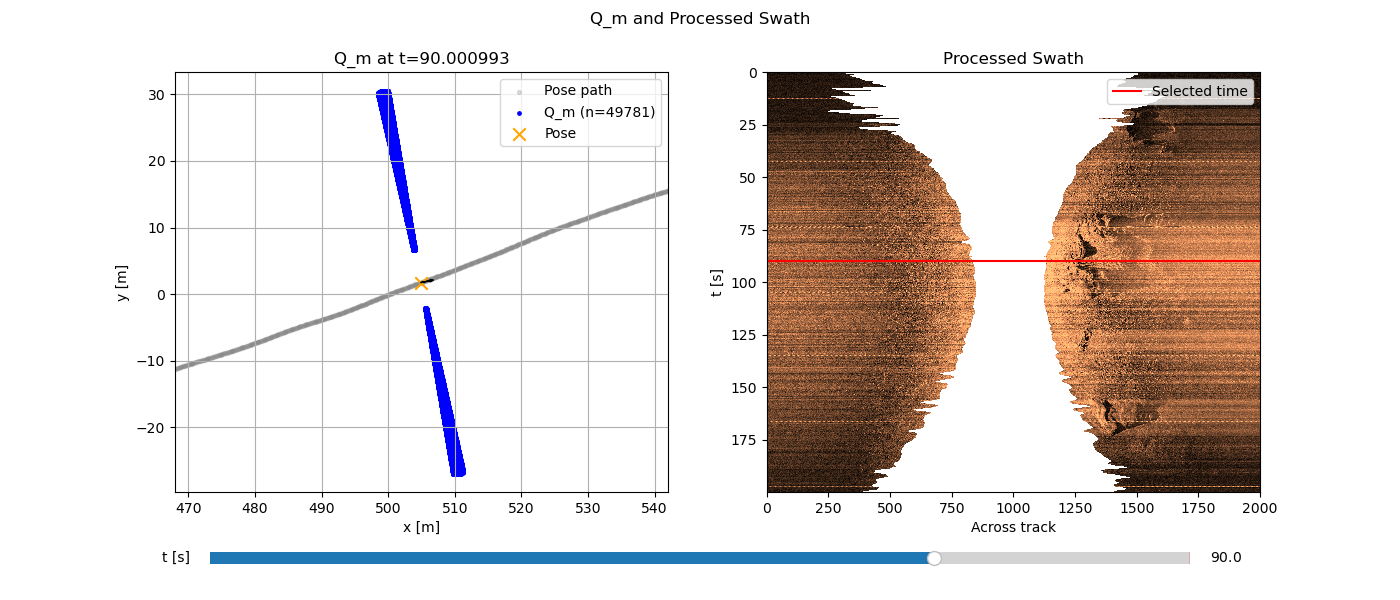
\includegraphics[width=0.93\linewidth]{Pictures/Results/Local_Map_Generation/Map_Generation/Q_m_pruned_3_zoomed_out.png}
    \caption{Effect of the two pruning stages on the candidate measurement set $Q_m$ shown at full spatial scale for one selected swath. The top image shows the initial candidate set after geometric footprint generation, the middle image shows the result after the fast approximate pruning stage, and the bottom image shows the final result after the probabilistic pruning stage.}
    \label{fig:results-local-map-generation-map-generation-pruning-zoomed-out}
\end{figure}

\newpage

\begin{figure}[H]
    \centering
    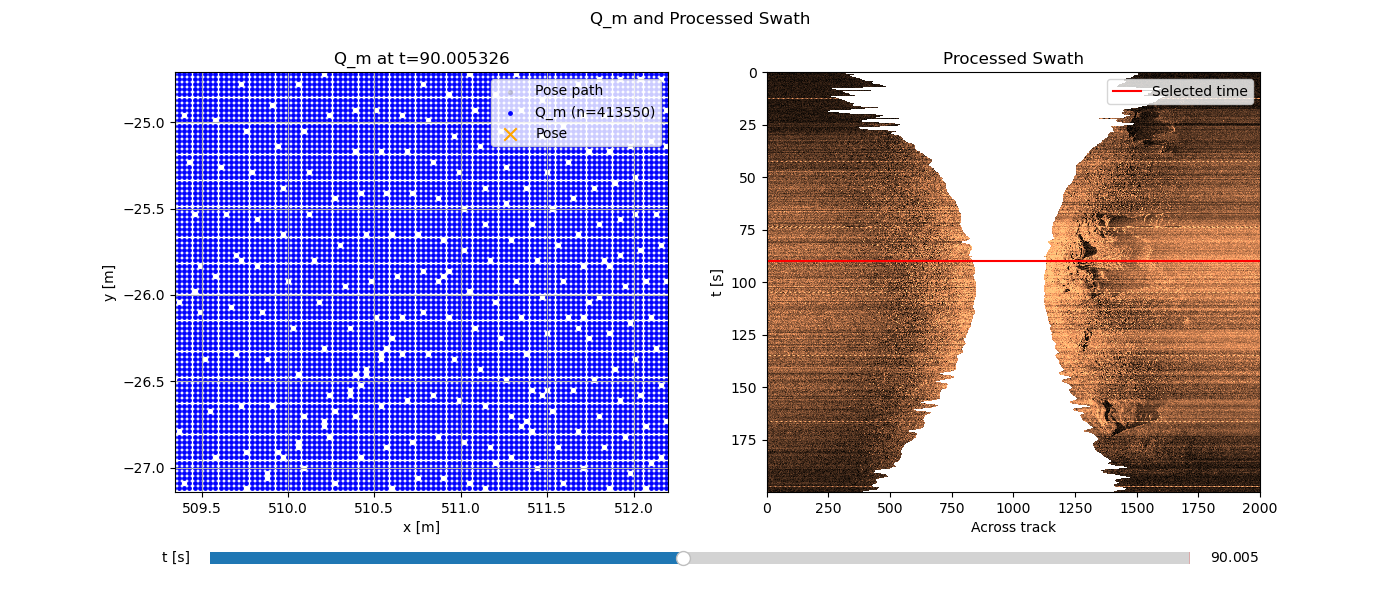
\includegraphics[width=0.95\linewidth]{Pictures/Results/Local_Map_Generation/Map_Generation/Q_m_pruned_1_zoomed_in.png}
    
    \vspace{0.01em}
    
    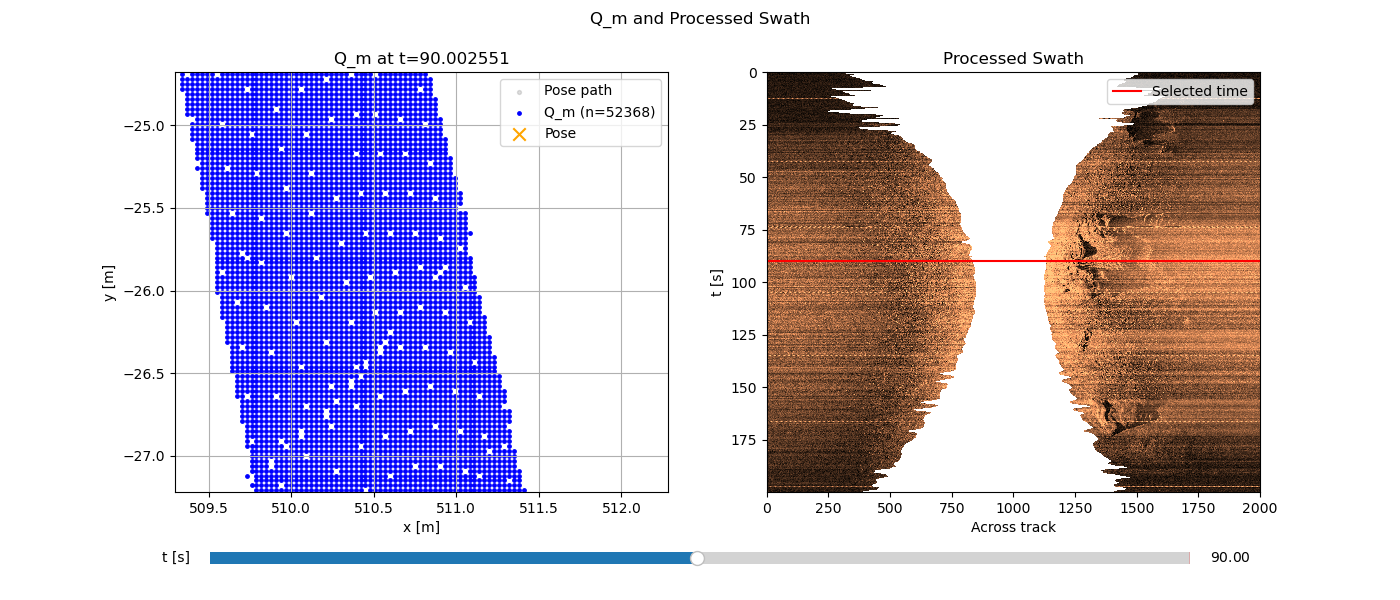
\includegraphics[width=0.95\linewidth]{Pictures/Results/Local_Map_Generation/Map_Generation/Q_m_pruned_2_zoomed_in.png}
    
    \vspace{0.01em}
    
    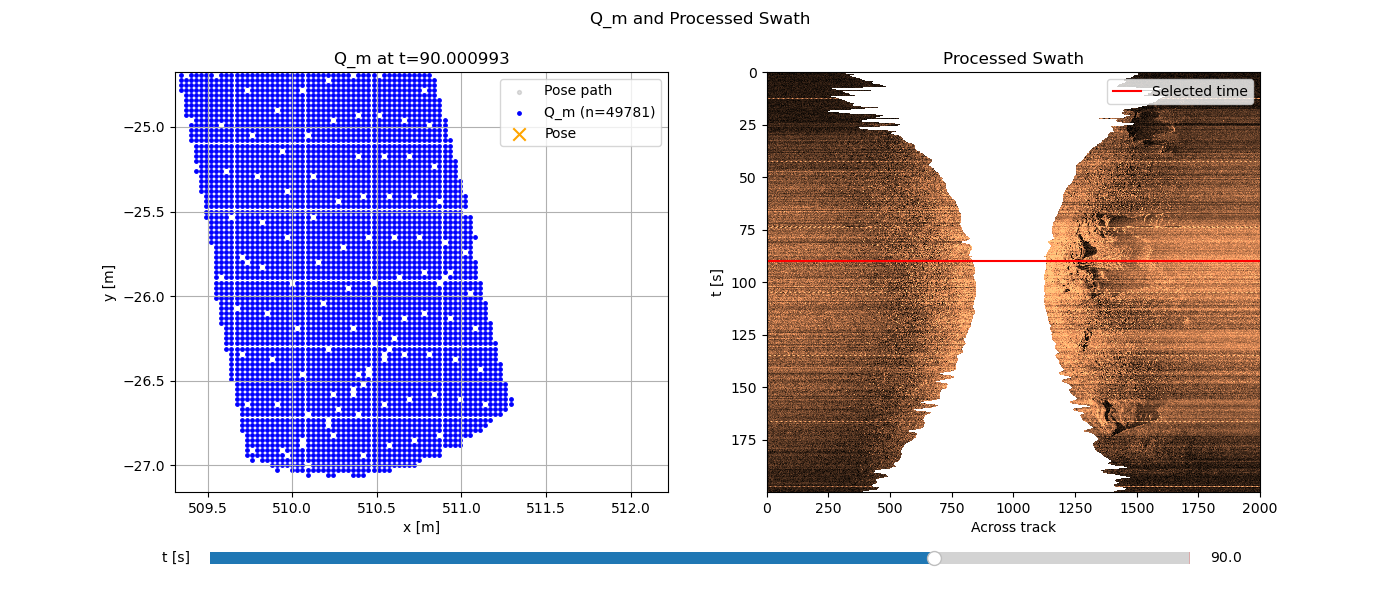
\includegraphics[width=0.95\linewidth]{Pictures/Results/Local_Map_Generation/Map_Generation/Q_m_pruned_3_zoomed_in.png}
    \caption{Zoomed view of the same pruning sequence as in Figure \ref{fig:results-local-map-generation-map-generation-pruning-zoomed-out}, highlighting how the discrete candidate cells are reduced while preserving the main illuminated support region.}
    \label{fig:results-local-map-generation-map-generation-pruning-zoomed-in}
\end{figure}

\newpage

\noindent
These figures illustrate the effect of the two stage pruning strategy on the temporary candidate set $Q_m$ for one selected swath. The initial candidate generation step produces a very large number of geometrically valid cells, here on the order of roughly $4\times 10^5$ candidates, because the full sonar footprint is sampled densely before any probabilistic filtering is applied. While this first set is useful as a geometric over approximation of where the ping could plausibly have illuminated the map, it is far too large to carry forward directly into the later interpolation and accumulation stages without unnecessary computational cost.
\\ \\
The first pruning stage applies the approximate beam model and acts mainly as a fast early rejection step. Its main effect is to remove weak candidates near the beam fringe, especially those lying far to the sides of the sampled sector where the expected beam contribution is already very small. This reduces the candidate set drastically, in the example shown here from roughly $410\,000$ cells down to about $52\,000$ cells, while largely preserving the main body of the illuminated support. As seen in both Figures \ref{fig:results-local-map-generation-map-generation-pruning-zoomed-out} and \ref{fig:results-local-map-generation-map-generation-pruning-zoomed-in}, the approximate pruning mainly narrows the angular support of the footprint, whereas the overall along range extent remains comparatively similar.
\\ \\
The second pruning stage then applies the more accurate probabilistic beam model. This stage is less aggressive in angular width, but further removes candidates whose contribution is still too small to be physically meaningful when both range and angular support are taken into account. In the example shown here, the candidate count is reduced further from about $52\,000$ to about $49\,000$ cells. The main visual effect is that some of the most distant low probability support is removed, while the final retained set remains concentrated in the region that is most likely to have been illuminated by the current ping. At the same time, the corresponding $P_m$ values of the surviving cells are preserved for later reuse in the accumulation stage.
\\ \\
The zoomed views make it easier to see that the final support is sparse and structured rather than dense over the full map. They also reveal small isolated gaps between some discrete candidate cells. These arise from the discretization step when the continuous footprint is snapped to the map grid. In practice, these gaps are typically very local, often on the order of a single cell, and are therefore not problematic for the final map construction since they are either compensated by overlapping neighboring pings or repaired later by the local gap filling stage. A finer map resolution could reduce such discretization gaps further, but this would also increase both runtime and memory cost significantly. The present parameter choice therefore represents a practical balance, where the vast majority of physically meaningful illuminated support is retained while the computational load is kept manageable for real time operation.

\newpage

\paragraph{Temporary measurement states $P_m$ and $V_m$} \mbox{}\\[0.5em] \noindent
\begin{figure}[H]
    \centering
    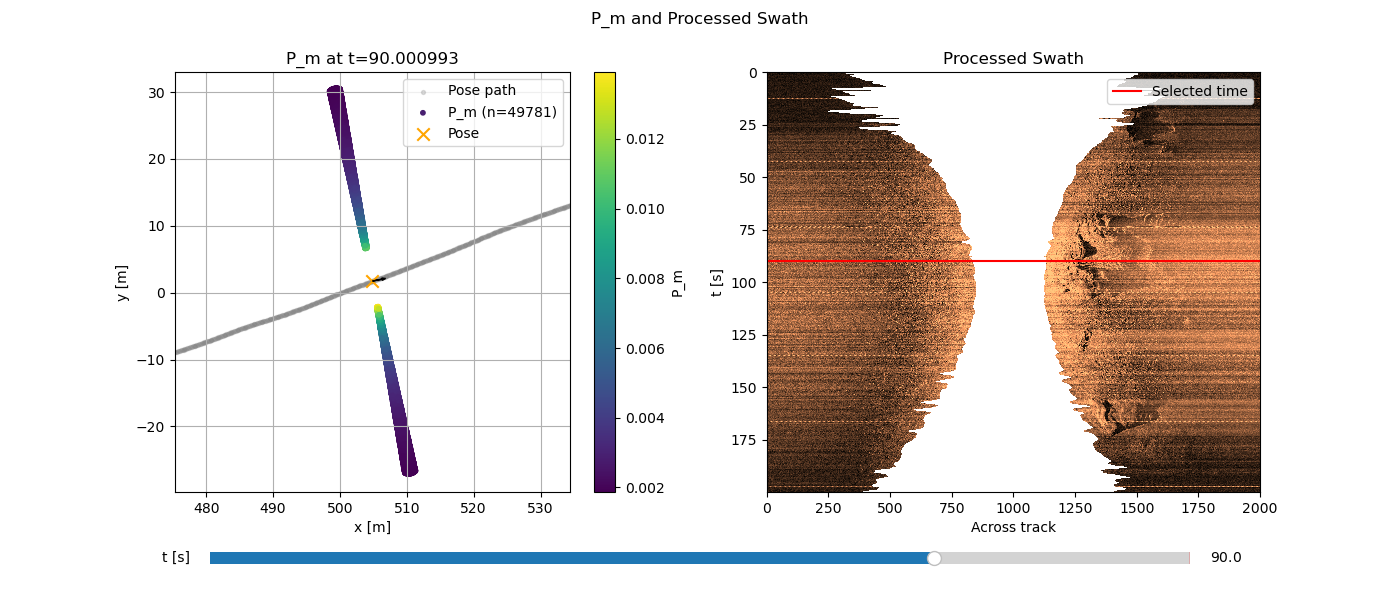
\includegraphics[width=1.0\linewidth]{Pictures/Results/Local_Map_Generation/Map_Generation/P_m.png}
    \caption{Visualization of the temporary probabilistic measurement support $P_m$ for the same selected swath as in the pruning results. The color scale shows the beam based support assigned to each surviving candidate cell after probabilistic pruning.}
    \label{fig:results-local-map-generation-map-generation-pm}
\end{figure}

\begin{figure}[H]
    \centering
    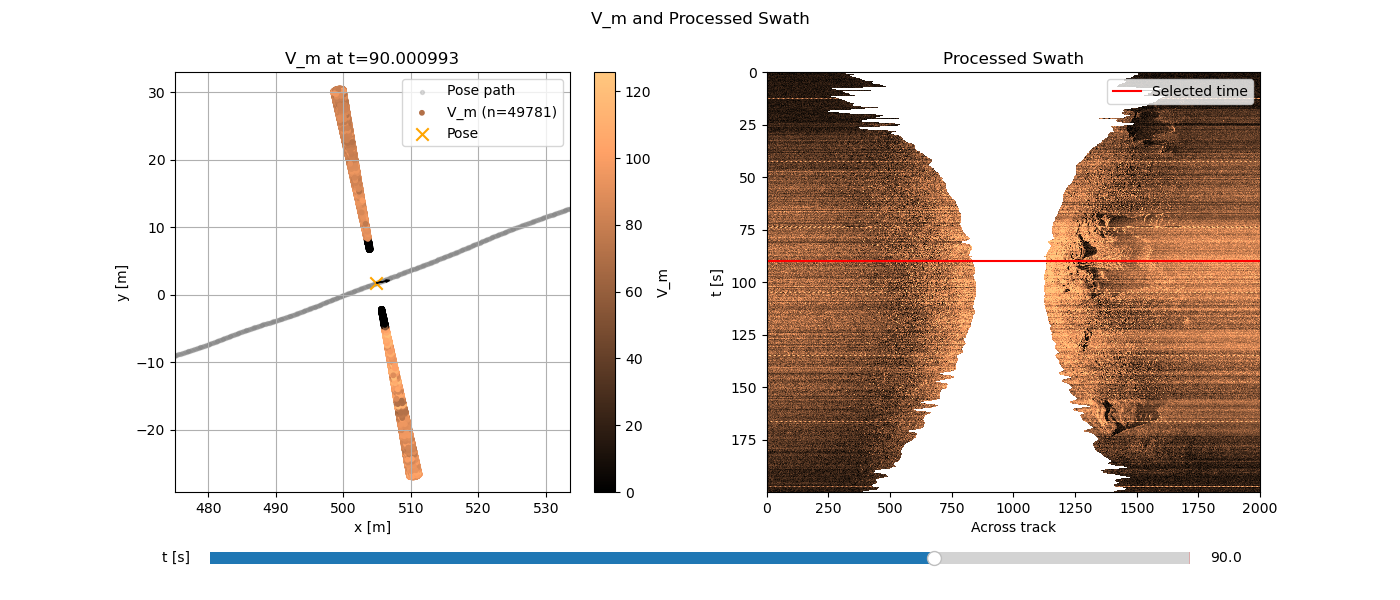
\includegraphics[width=1.0\linewidth]{Pictures/Results/Local_Map_Generation/Map_Generation/V_m.png}
    \caption{Visualization of the temporary interpolated intensity measurement map $V_m$ for the same selected swath. The color scale shows the reflectivity value assigned to each surviving candidate cell after backprojection into the processed swath and local interpolation.}
    \label{fig:results-local-map-generation-map-generation-vm}
\end{figure}

\newpage

\noindent
After probabilistic pruning, each surviving candidate cell is assigned two temporary quantities for the current ping, the probabilistic support value $P_m$ and the interpolated intensity value $V_m$. Figure \ref{fig:results-local-map-generation-map-generation-pm} shows how $P_m$ is distributed over the retained candidate support. As expected from the beam model, the strongest support is concentrated in the part of the swath that is most plausibly illuminated by the current ping, while support decreases away from this region. This confirms that the pruning stage does not only reduce the number of candidates, but also leaves behind a structured probabilistic support field that is physically consistent with the expected sonar footprint.
\\ \\
Figure \ref{fig:results-local-map-generation-map-generation-vm} shows the corresponding temporary intensity measurement map $V_m$. Unlike $P_m$, which reflects beam support, $V_m$ reflects the processed swath intensity assigned to the surviving cells after backprojection and interpolation. The two maps therefore look related but clearly different. The support field $P_m$ is dominated by the beam geometry, whereas $V_m$ follows the measured reflectivity structure taken from the processed swath. In the example shown here, the near part of the retained swath appears darker while the farther part becomes brighter, indicating that the interpolated reflectivity varies substantially over the selected support region.
\\ \\
This difference between $P_m$ and $V_m$ is important, since they represent two different parts of the measurement model. The quantity $P_m$ describes how strongly a cell is supported by the beam geometry, while $V_m$ describes what reflectivity value that cell receives from the processed swath. The map generator does not accumulate intensity alone, but rather combines both quantities later through probability weighted accumulation. Another important observation is that $V_m$ is computed only for the already pruned support, not for the full raw candidate set. This is one of the main reasons the algorithm remains efficient in practice, since the more expensive interpolation step is evaluated only for cells that have already been judged sufficiently relevant by the pruning stage.

\newpage

\paragraph{Persistent states $P$ and $V$} \mbox{}\\[0.5em] \noindent
\begin{figure}[H]
    \centering
    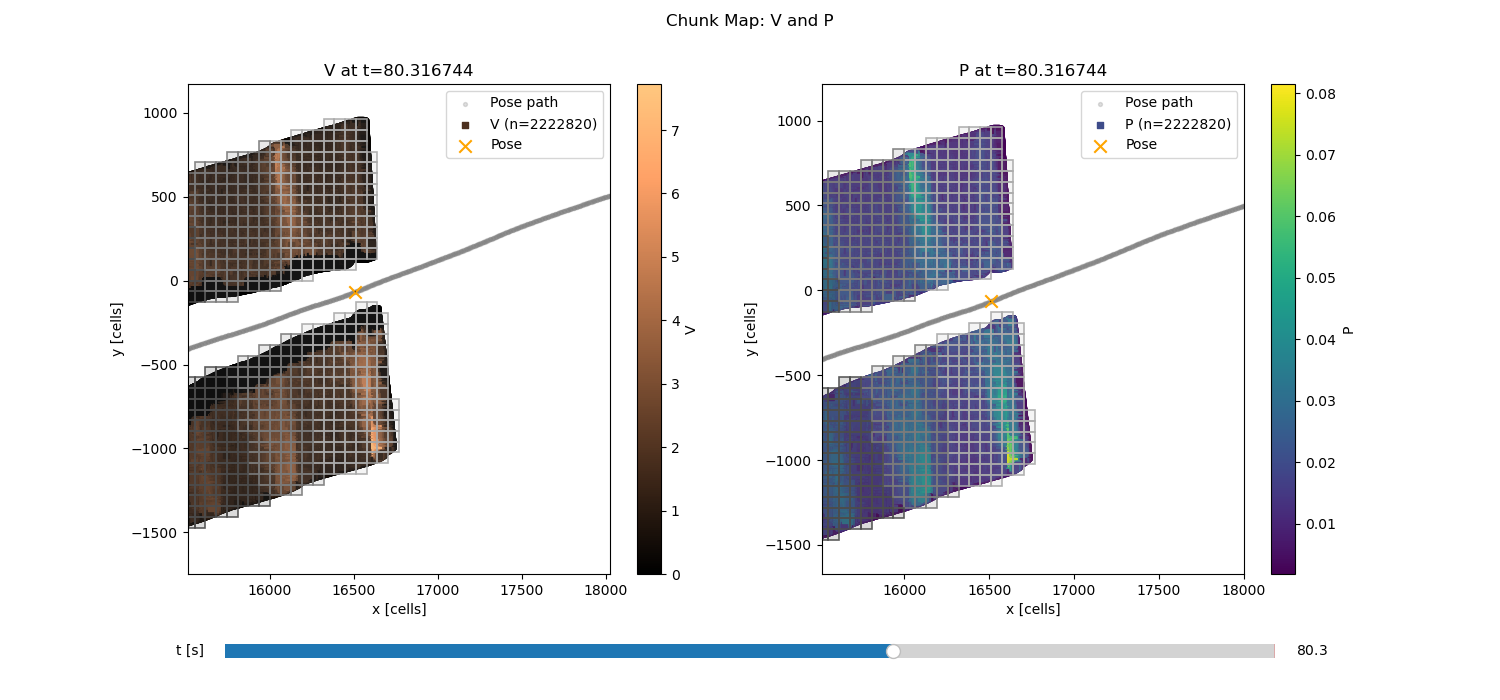
\includegraphics[width=0.93\linewidth]{Pictures/Results/Local_Map_Generation/Map_Generation/V_and_P_1.png}
    
    \vspace{0.01em}
    
    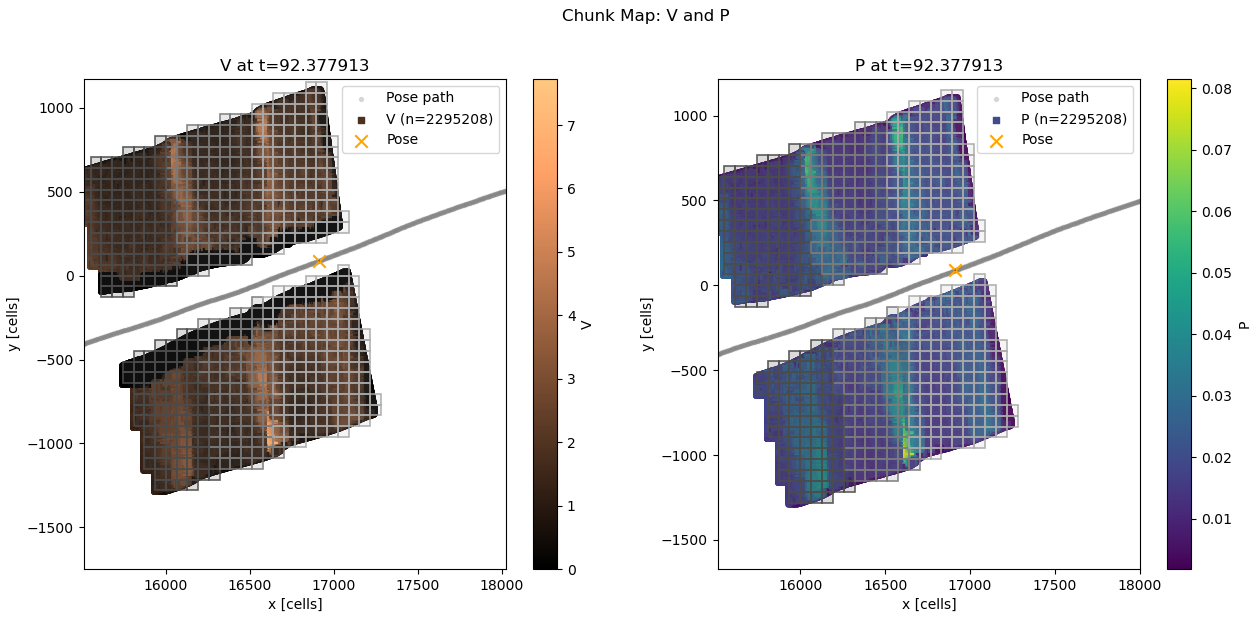
\includegraphics[width=0.93\linewidth]{Pictures/Results/Local_Map_Generation/Map_Generation/V_and_P_2.png}
    
    \vspace{0.01em}
    
    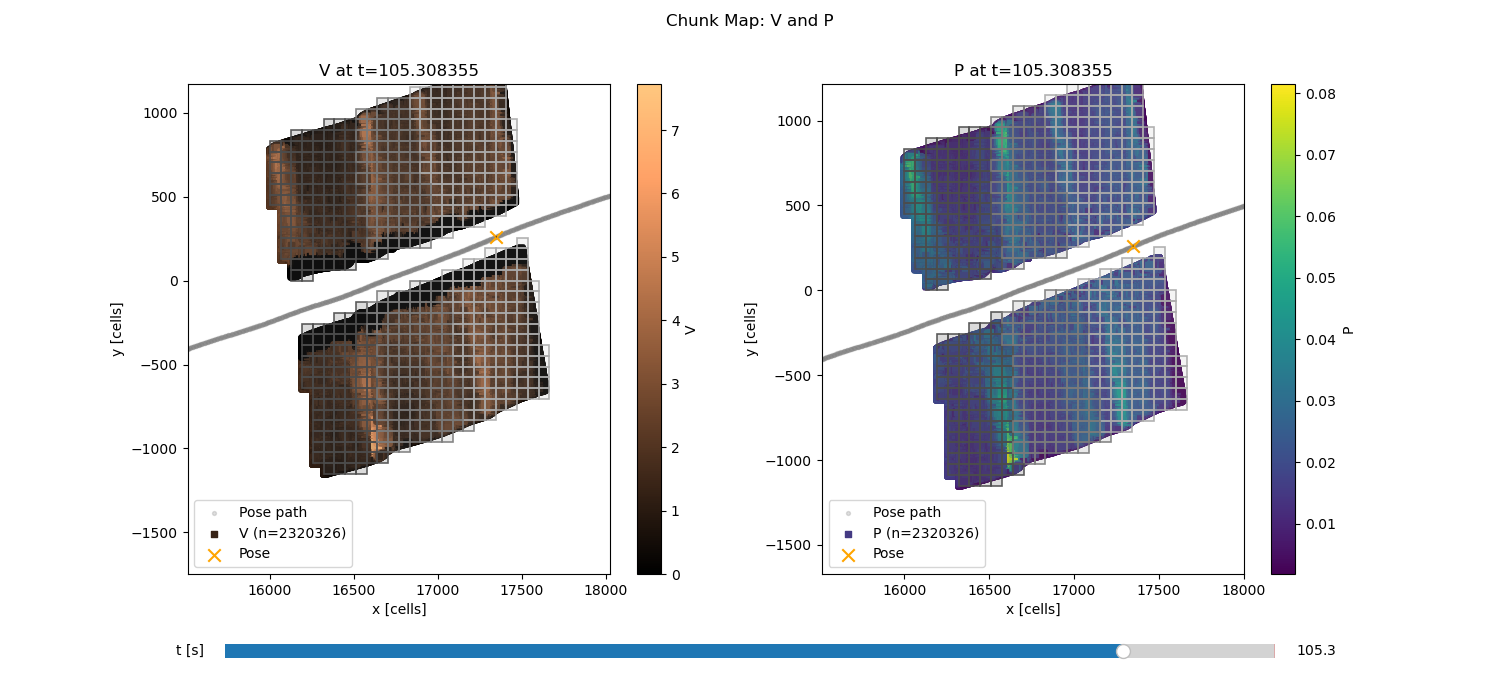
\includegraphics[width=0.93\linewidth]{Pictures/Results/Local_Map_Generation/Map_Generation/V_and_P_3.png}
    \caption{Evolution of the persistent map states $V$ and $P$ over time. The gray grid indicates the active chunk structure used to store the accumulated local map states.}
    \label{fig:results-local-map-generation-map-generation-persistent-states}
\end{figure}

\newpage

\noindent
While $P_m$ and $V_m$ describe only the temporary measurement contribution from a single ping, the quantities $P$ and $V$ represent the persistent states obtained after accumulation over many successive pings. Here, $P$ stores the accumulated observation support, while $V$ stores the accumulated probability weighted intensity. These quantities are therefore not yet the final normalized map image, but rather the intermediate persistent states from which the final map is later constructed.
\\ \\
Figure \ref{fig:results-local-map-generation-map-generation-persistent-states} shows how these persistent states grow over time as new swaths are incorporated. The overall illuminated support gradually expands along the vehicle trajectory, while the internal spatial structure becomes richer as repeated measurements are accumulated. This makes the difference between the temporary and persistent states very clear: the temporary states describe only the current swath, whereas the persistent states represent the cumulative measurement history retained inside the local map.
\\ \\
An important part of this process is the chunked sparse map representation. Instead of storing the full map as one dense image at all times, the accumulated states are stored only inside active spatial chunks. Each gray square in Figure \ref{fig:results-local-map-generation-map-generation-persistent-states} corresponds to one active chunk, and each chunk contains a fixed local grid of map cells, here set by the chosen chunk size of $64 \times 64$ pixels. This makes it possible to grow the map dynamically only where measurements actually exist, while avoiding unnecessary allocation in empty space. As the map evolves, new chunks are allocated where new support appears, previously active chunks remain alive for a limited time, and old untouched chunks are eventually removed by the chunk aging logic. This behavior can be seen directly in the sequence, where some older outer chunks disappear as the vehicle moves forward and the local map focus shifts.
\\ \\
The number of active chunks that appear at any given time is also influenced by the map update policy. In the present setup, the dense map is rebuilt either after every 100 buffered swaths or when the time gap between updates reaches $5\,\mathrm{s}$ depending on the tuned parameters in Table \ref{tab:local-map-generation-parameters}. These settings determine how much accumulated support is allowed to build up before the next map output is formed, and therefore also influence how large the active chunk region becomes in practice. In simple terms, more retained swaths between updates generally produce a larger active support region, while fewer retained swaths keep the local map more compact. Together with the chunk size and chunk age, these parameters therefore help determine both the visible spatial extent of the persistent states and the computational cost of maintaining them.
\\ \\
The chunk management is important both for memory and runtime. Memory usage stays bounded because only the active local region is retained, and computational cost is reduced because later stages such as dense map construction and gap filling only need to operate on the chunks that currently contain valid accumulated data. At the same time, the results show that even with this bounded representation the number of retained illuminated cells quickly becomes very large, reaching on the order of several million map pixels. This highlights why the earlier pruning stages are necessary: without aggressive reduction of the temporary support before accumulation, the persistent states would grow too quickly to remain practical for real-time use.
\\ \\
A final observation from these figures is that the persistent states $P$ and $V$ are clearly related but visually different. The state $P$ reflects how strongly different parts of the map have been supported by repeated probabilistic beam observations, while $V$ reflects the accumulated weighted intensity structure. In other words, $P$ describes where the map is well supported, whereas $V$ describes what weighted reflectivity information has been accumulated there. Only in the later normalization step are these two persistent states combined to produce the final local reflectivity map.

\newpage

\paragraph{Normalized map construction $M$} \mbox{}\\[0.5em] \noindent
\begin{figure}[H]
    \centering
    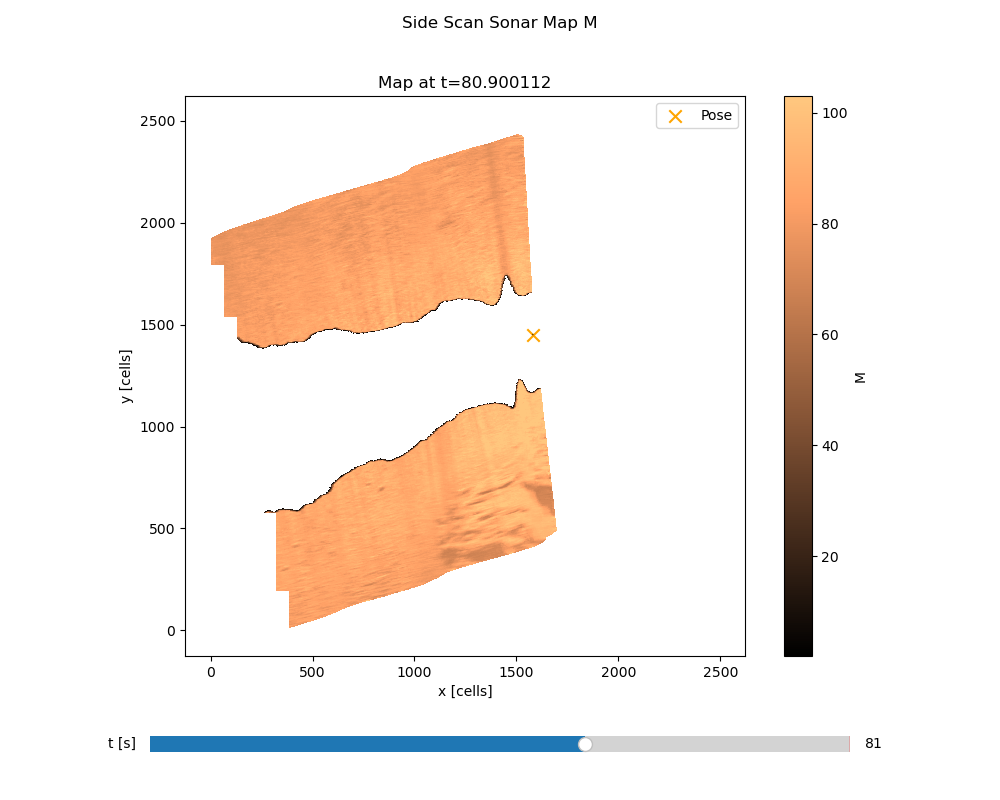
\includegraphics[width=0.75\linewidth]{Pictures/Results/Local_Map_Generation/Map_Generation/M_1.png}
    \caption{Normalized local map $M$ at the first selected time instant.}
    \label{fig:results-local-map-generation-map-generation-normalized-map-1}
\end{figure}

\vspace{-1.0em}

\begin{figure}[H]
    \centering
    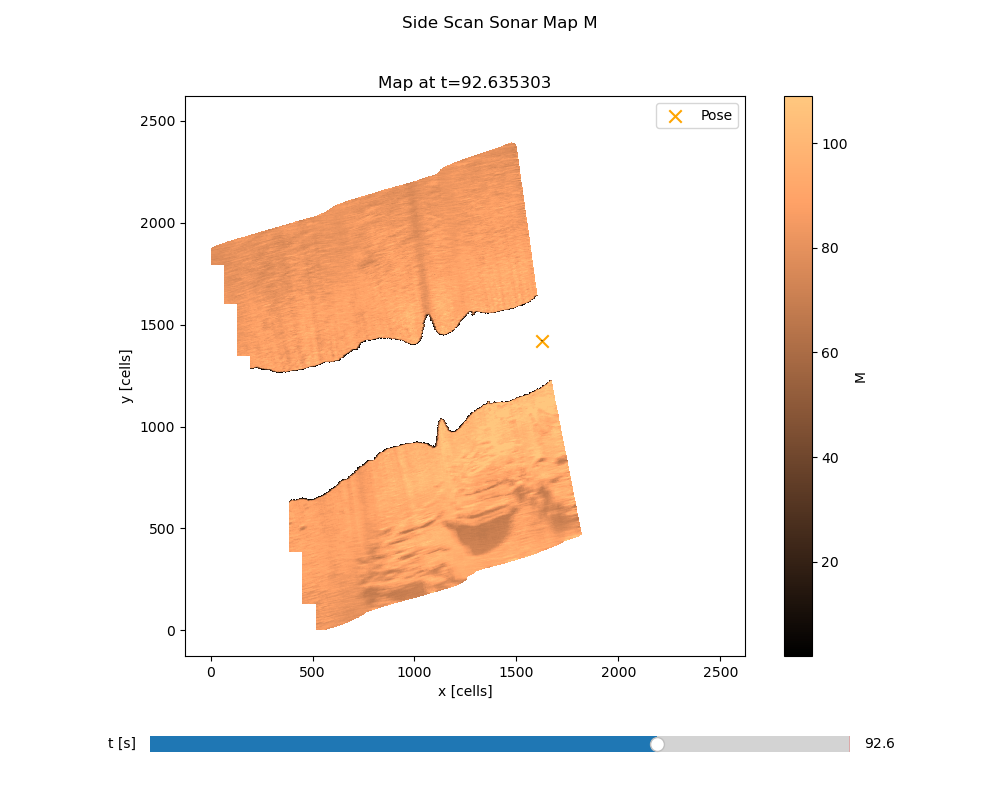
\includegraphics[width=0.75\linewidth]{Pictures/Results/Local_Map_Generation/Map_Generation/M_2.png}
    \caption{Normalized local map $M$ at the second selected time instant.}
    \label{fig:results-local-map-generation-map-generation-normalized-map-2}
\end{figure}

\newpage

\begin{figure}[H]
    \centering
    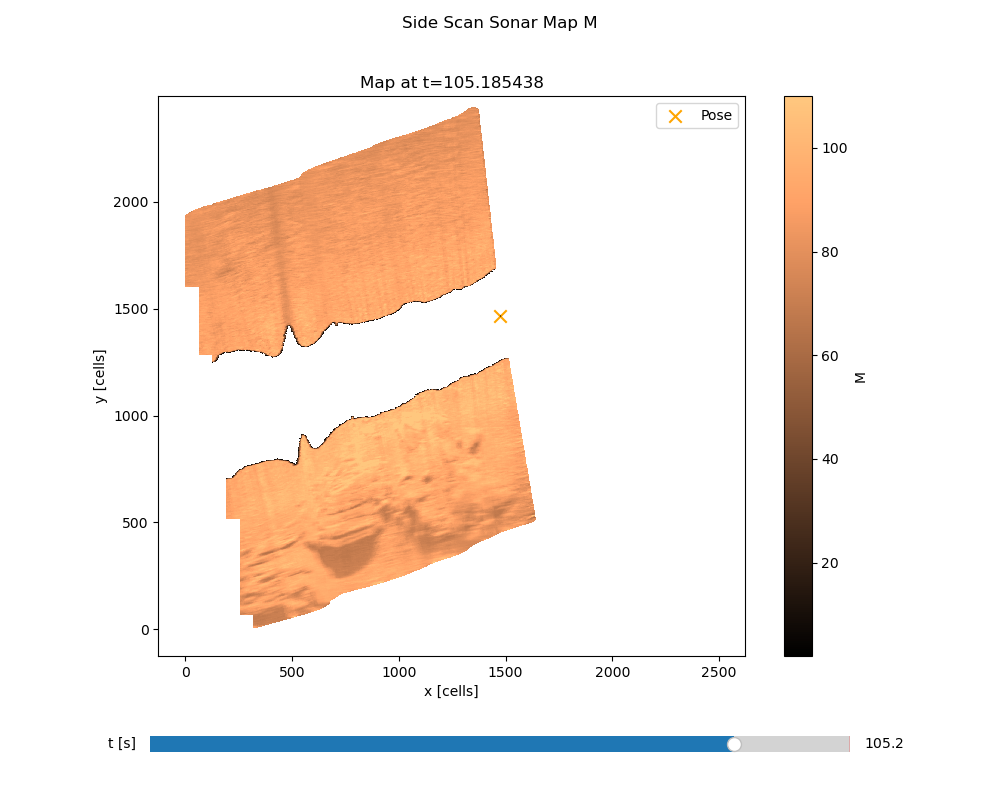
\includegraphics[width=0.80\linewidth]{Pictures/Results/Local_Map_Generation/Map_Generation/M_3.png}
    \caption{Normalized local map $M$ at the third selected time instant.}
    \label{fig:results-local-map-generation-map-generation-normalized-map-3}
\end{figure}
\noindent
These figures show the construction of the normalized local map $M$ from the previously accumulated persistent states $V$ and $P$. Thus, the three maps shown here correspond directly to the same three time instants used in Figure \ref{fig:results-local-map-generation-map-generation-persistent-states}, now converted into the final dense reflectivity map through the normalization step. In this sense, the present results show the actual image produced from the accumulated chunk based support, rather than the intermediate persistent states themselves.
\\ \\
The normalization combines the accumulated weighted intensity and accumulated support into a dense local image, and the remaining small gaps are then repaired by the local gap filling stage. The result is therefore the final local map output produced by the map generation algorithm at each of the shown time instants. Compared with the processed swath representation, the mapped features now appear much more geometrically meaningful. In the processed swath domain, many structures look compressed, warped, or difficult to interpret because they are still tied to the sonar acquisition geometry. After map construction, however, the same structures appear in a spatial form that is much closer to their actual layout on the seafloor.
\\ \\
A clear qualitative observation is that the reconstructed map reveals seabed features with good contrast and continuity, indicating that the combined stages of probabilistic pruning, intensity interpolation, persistent accumulation, normalization, and local fill in work together as intended. At the same time, some local stretching and mild geometric distortion can still be observed in parts of the map. This is expected, since the final map quality is fundamentally limited by the quality of the underlying state estimate used during map accumulation. In other words, the map reconstruction can only be as geometrically accurate as the estimated vehicle motion and pose alignment allow.
\\ \\
Even so, the overall result is clearly usable and captures the main seabed structure well. The remaining distortion appears relatively moderate, and it is reasonable to expect that further parameter tuning in the state estimator, especially in the forward motion consistency and aiding quality, would make the local maps even more geometrically accurate. As a result, these normalized map results indicate that the implemented map generation stage already produces a meaningful and practically useful local representation of the seafloor for the later stages of the SLAM pipeline.

\newpage

\paragraph{Full mission map reconstructed mosaic} \mbox{}\\[0.5em] \noindent
\begin{figure}[H]
    \centering
    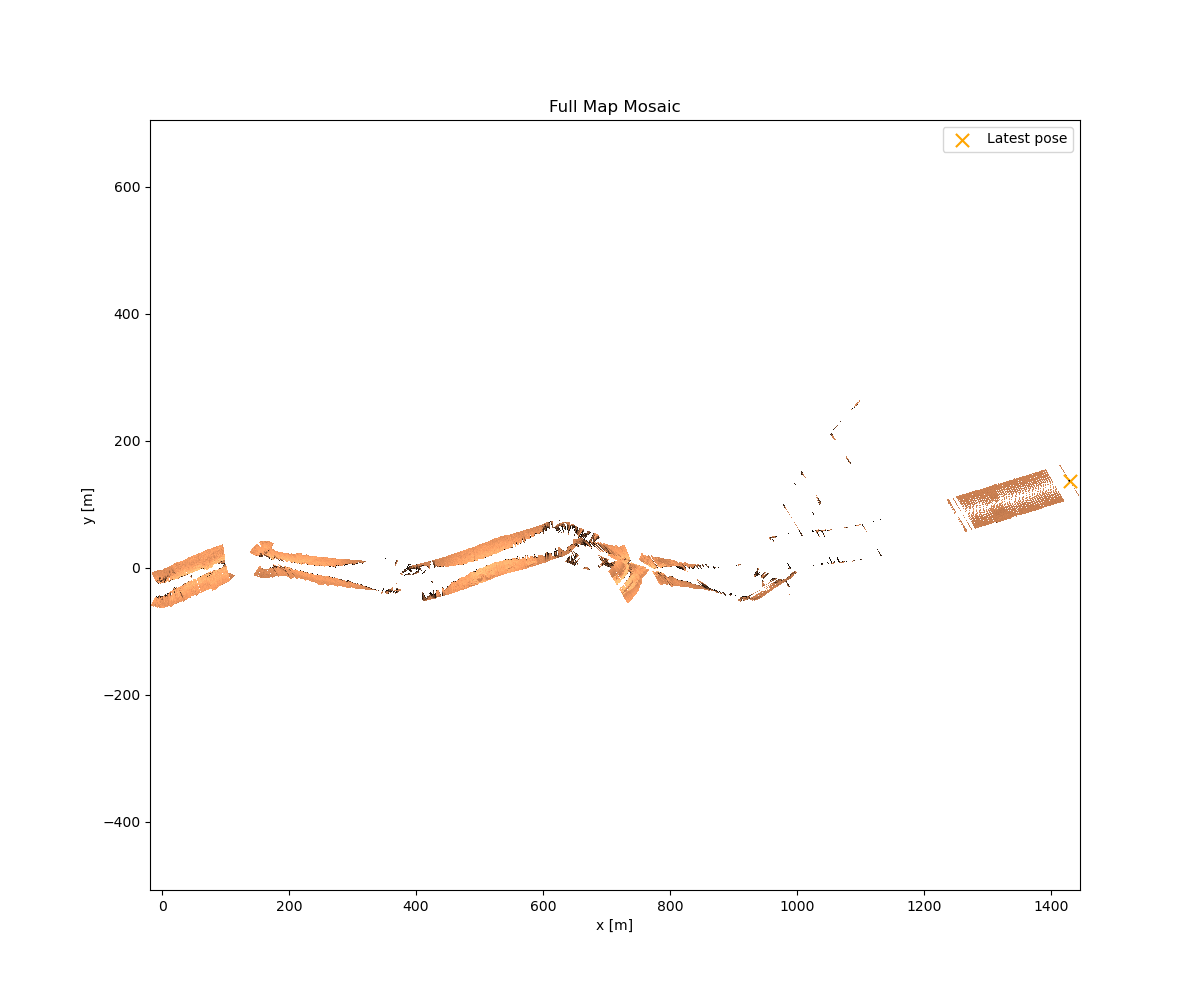
\includegraphics[width=1.00\linewidth]{Pictures/Results/Local_Map_Generation/Map_Generation/Full_Map_zoomed_out.png}
    \caption{Full local map result accumulated over the complete mission.}
    \label{fig:results-local-map-generation-map-generation-full-map}
\end{figure}
\noindent
Figure \ref{fig:results-local-map-generation-map-generation-full-map} shows the full map reconstructed over the complete mission. The main observation here is simply the scale of the result. The mapped area is very large, spanning roughly $1400 \times 600\,\mathrm{m}$, and with a map resolution of $0.03\,\mathrm{m/pixel}$ this corresponds to a very large dense map representation. In practice, the final map reaches on the order of gigabytes without compression, which highlights the importance of the sparse chunked representation used internally during processing.
\\ \\
At this scale, the purpose of the figure is mainly to show the overall spatial extent of the reconstruction and the fact that the map generation pipeline is able to produce a mission scale mosaic from the processed swaths. The finer local quality of different map regions is difficult to judge from the full overview alone and is therefore examined in the following subsections using more zoomed in examples. Those later results are used to discuss where the map is well aligned, where it degrades, and how this depends on the quality of the underlying state estimate and aiding measurements.

\newpage

\paragraph{Map quality under good aiding conditions} \mbox{}\\[0.5em] \noindent
\begin{figure}[H]
    \centering
    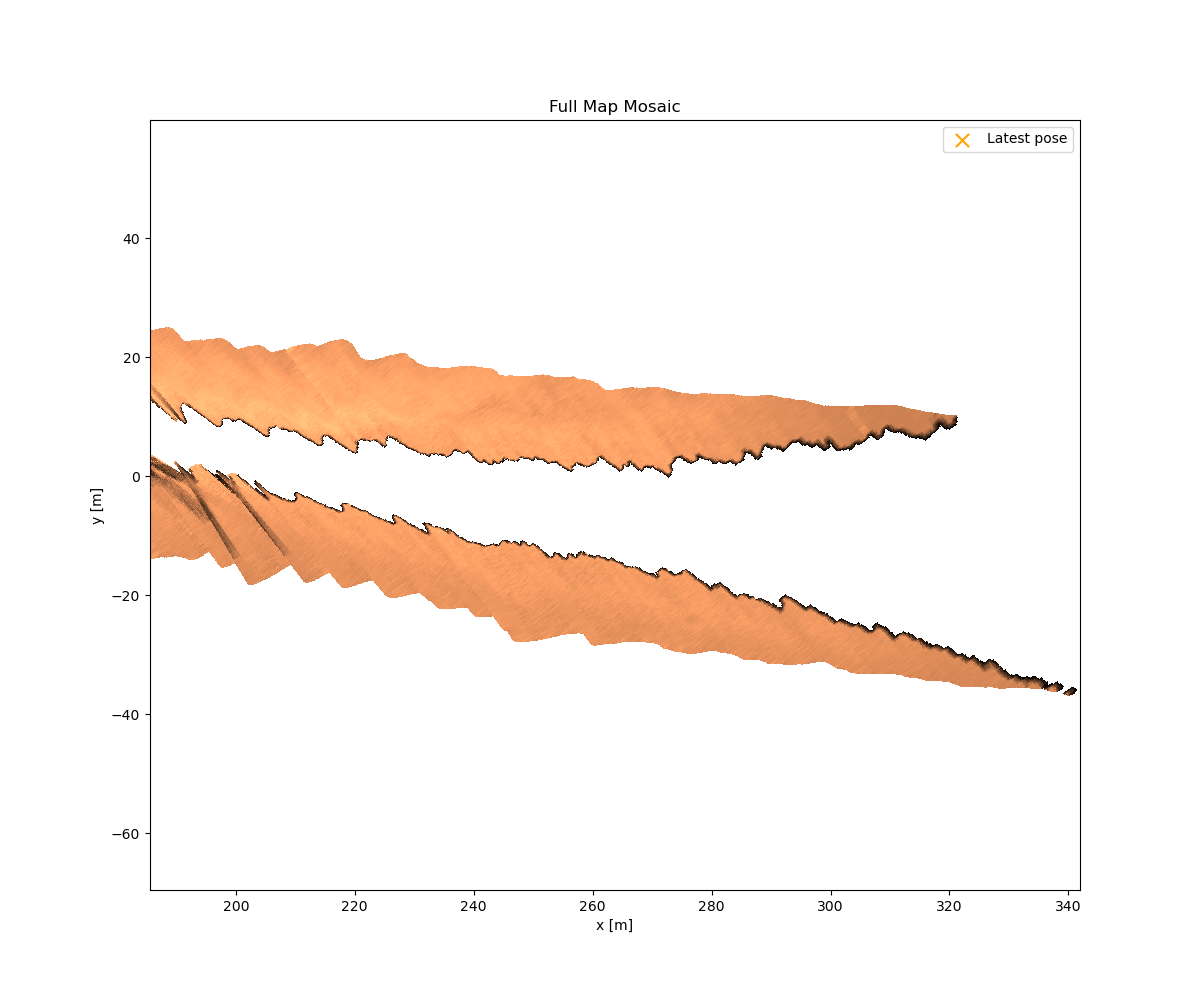
\includegraphics[width=0.8\linewidth]{Pictures/Results/Local_Map_Generation/Map_Generation/Full_Map_zoomed_in_1.png}
    
    \vspace{0.01em}
    
    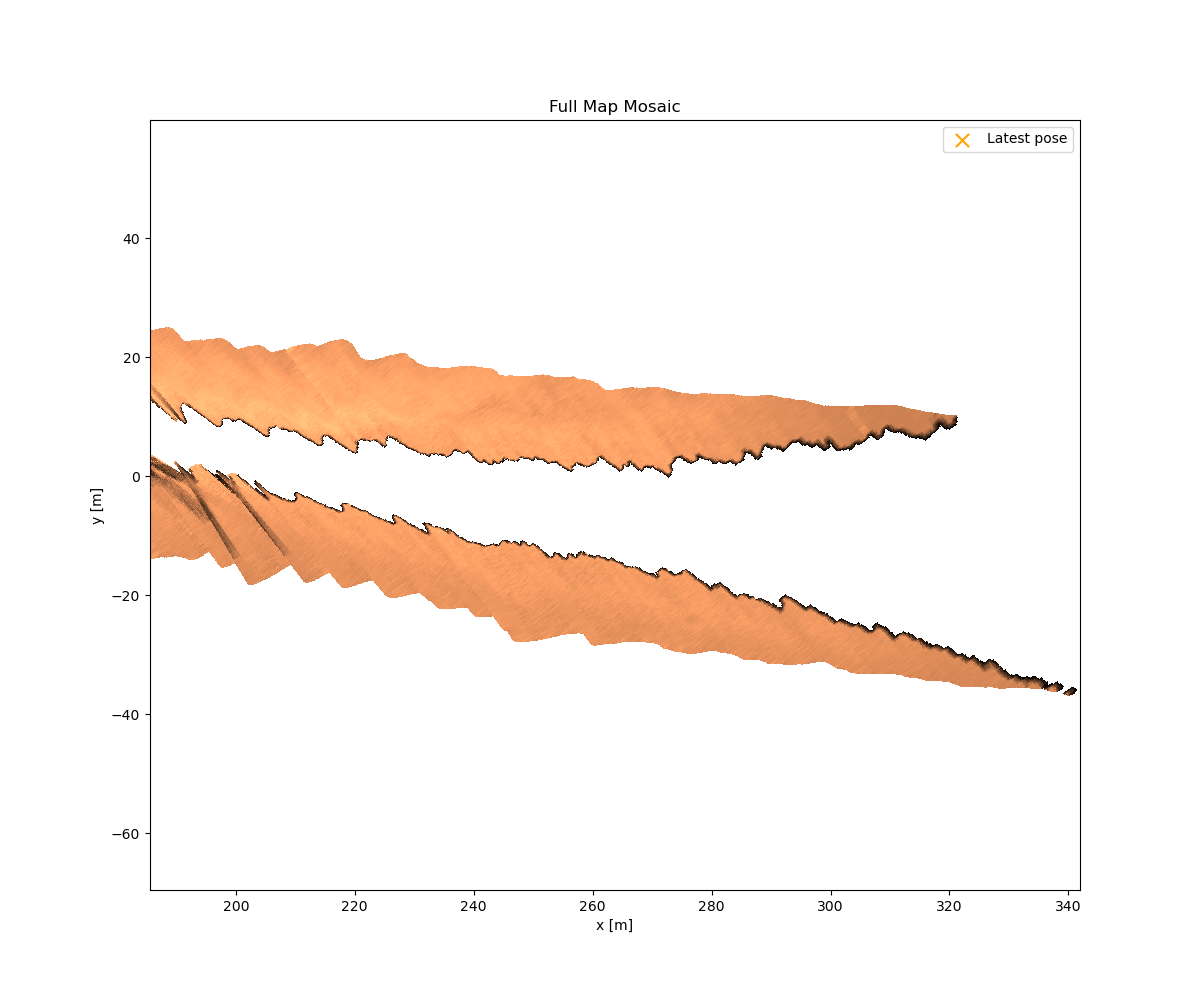
\includegraphics[width=0.8\linewidth]{Pictures/Results/Local_Map_Generation/Map_Generation/Full_Map_zoomed_in_2.png}
    \caption{Examples of local map regions reconstructed during periods with good aiding availability.}
    \label{fig:results-local-map-generation-map-generation-map-under-good-aiding}
\end{figure}

\newpage

\noindent
Figure \ref{fig:results-local-map-generation-map-generation-map-under-good-aiding} shows two zoomed in regions of the final mission map during periods where DVL aiding was available. In these parts of the mission, the state estimate remained well constrained and the accumulated map therefore appears spatially coherent over longer distances. The reconstructed swaths overlap consistently, the mapped corridor remains geometrically stable, and the local reflectivity structure is preserved clearly enough to reveal meaningful seabed texture and larger visible features.
\\ \\
A clear observation in both examples is that the map strips align well from pass to pass, with only limited visible distortion. This is the expected behavior when DVL aiding is present, since the estimator drift remains small and the map accumulation can stay consistent over time. These examples therefore illustrate the nominal operating case of the map generation pipeline, when DVL aiding is available, the algorithm is able to produce a stable and visually consistent local map that is well suited for later feature extraction and matching.

\newpage

\paragraph{Map degradation during dead reckoning} \mbox{}\\[0.5em] \noindent
\begin{figure}[H]
    \centering
    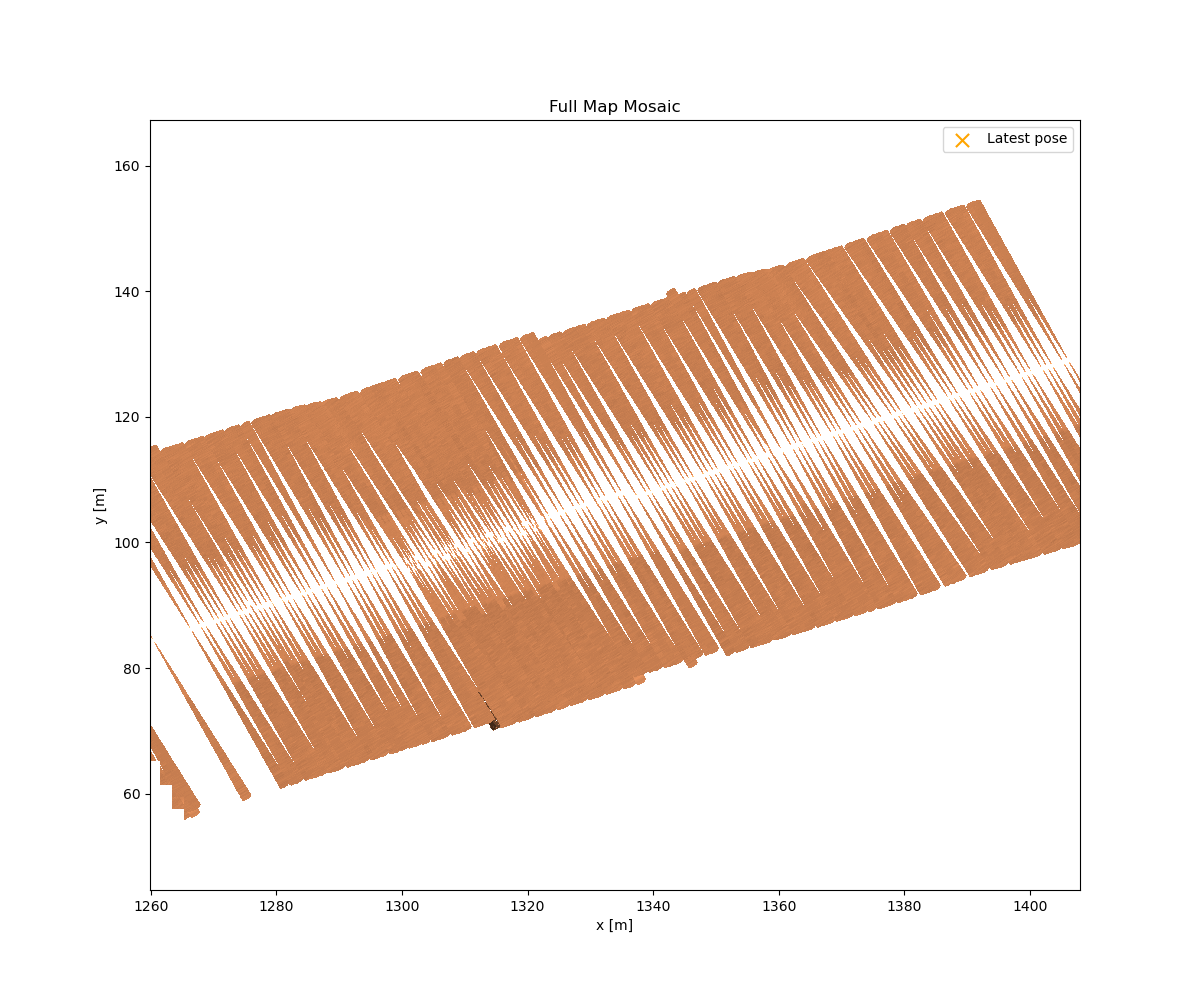
\includegraphics[width=1.00\linewidth]{Pictures/Results/Local_Map_Generation/Map_Generation/Full_Map_zoomed_in_3.png}
    \caption{Example of map degradation during a period with lost aiding.}
    \label{fig:results-local-map-generation-map-generation-dead-reckoning}
\end{figure}
\noindent
Figure \ref{fig:results-local-map-generation-map-generation-dead-reckoning} shows a part of the mission where DVL aiding was lost and the estimator therefore had to rely more heavily on dead reckoning. In this situation, the pose error accumulates over time, and the effect becomes directly visible in the reconstructed map. The mapped swaths no longer overlap as tightly as before, the corridor becomes unnaturally sparse, and the reconstruction appears stretched along the trajectory.
\\ \\
Here, the accumulated state estimation error causes the vehicle motion to be reconstructed as larger than it actually was. As a result, consecutive swaths are placed too far apart in the map, which makes the local support region wider and more spread out than expected. This not only degrades the spatial consistency of the final map, but also increases the computational cost of the map generation stage, since larger candidate regions must then be generated, pruned, interpolated, and accumulated.
\\ \\
This example therefore illustrates an important dependency of the local map generation stage, the quality of the final map is strongly tied to the quality of the underlying state estimate. When aiding is available, the map remains compact and coherent, but when aiding is lost and dead reckoning error grows, the resulting reconstruction becomes progressively less reliable and may no longer be suitable for accurate spatial interpretation or later feature matching.

\newpage

\paragraph{Map distortion after aiding correction} \mbox{}\\[0.5em] \noindent
\begin{figure}[H]
    \centering
    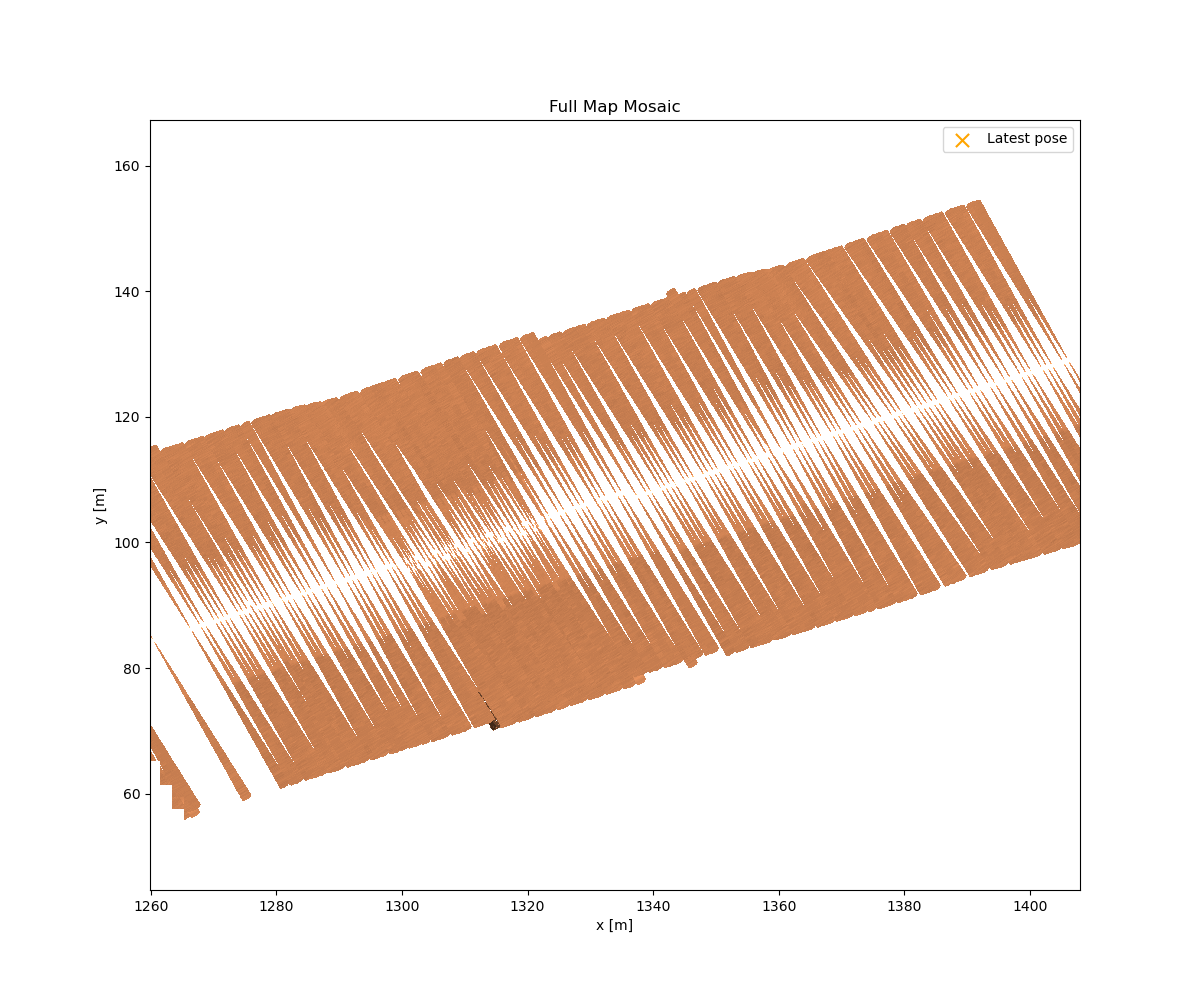
\includegraphics[width=1.00\linewidth]{Pictures/Results/Local_Map_Generation/Map_Generation/Full_Map_zoomed_in_4.png}
    \caption{Example of map distortion after estimator correction following a period of dead reckoning.}
    \label{fig:results-local-map-generation-map-generation-aiding-correction}
\end{figure}
\noindent
Figure \ref{fig:results-local-map-generation-map-generation-aiding-correction} shows the case where aiding measurements return after a longer period of dead reckoning. During the dead reckoning phase, the pose error accumulates progressively and the map is built on top of that drifting estimate. When aiding becomes available again, the estimator corrects the pose, and this correction appears directly in the accumulated map as a geometric discontinuity.
\\ \\
The visible result is a local distortion where previously accumulated map content no longer aligns well with the newly corrected trajectory. This can appear as a sudden spatial snap, local bending of the mapped corridor, overlap mismatch, or multiple swath regions intersecting in an unnatural way. The stronger the accumulated error before aiding returns, the stronger this distortion becomes.
\\ \\
This example highlights another important dependency of the map generation stage. The map generator itself continues to accumulate measurements consistently with respect to the current state estimate, but if that state estimate changes sharply after a correction, older accumulated map contributions from the dead reckoning period may remain geometrically inconsistent with the newer corrected ones. As a result, the final distortion seen here is not caused by the probabilistic mapping model itself, but by the interaction between accumulated map states and a delayed correction in the underlying navigation estimate.

\newpage

\paragraph{Performance} \mbox{}\\[0.5em] \noindent
\begin{figure}[H]
    \centering
    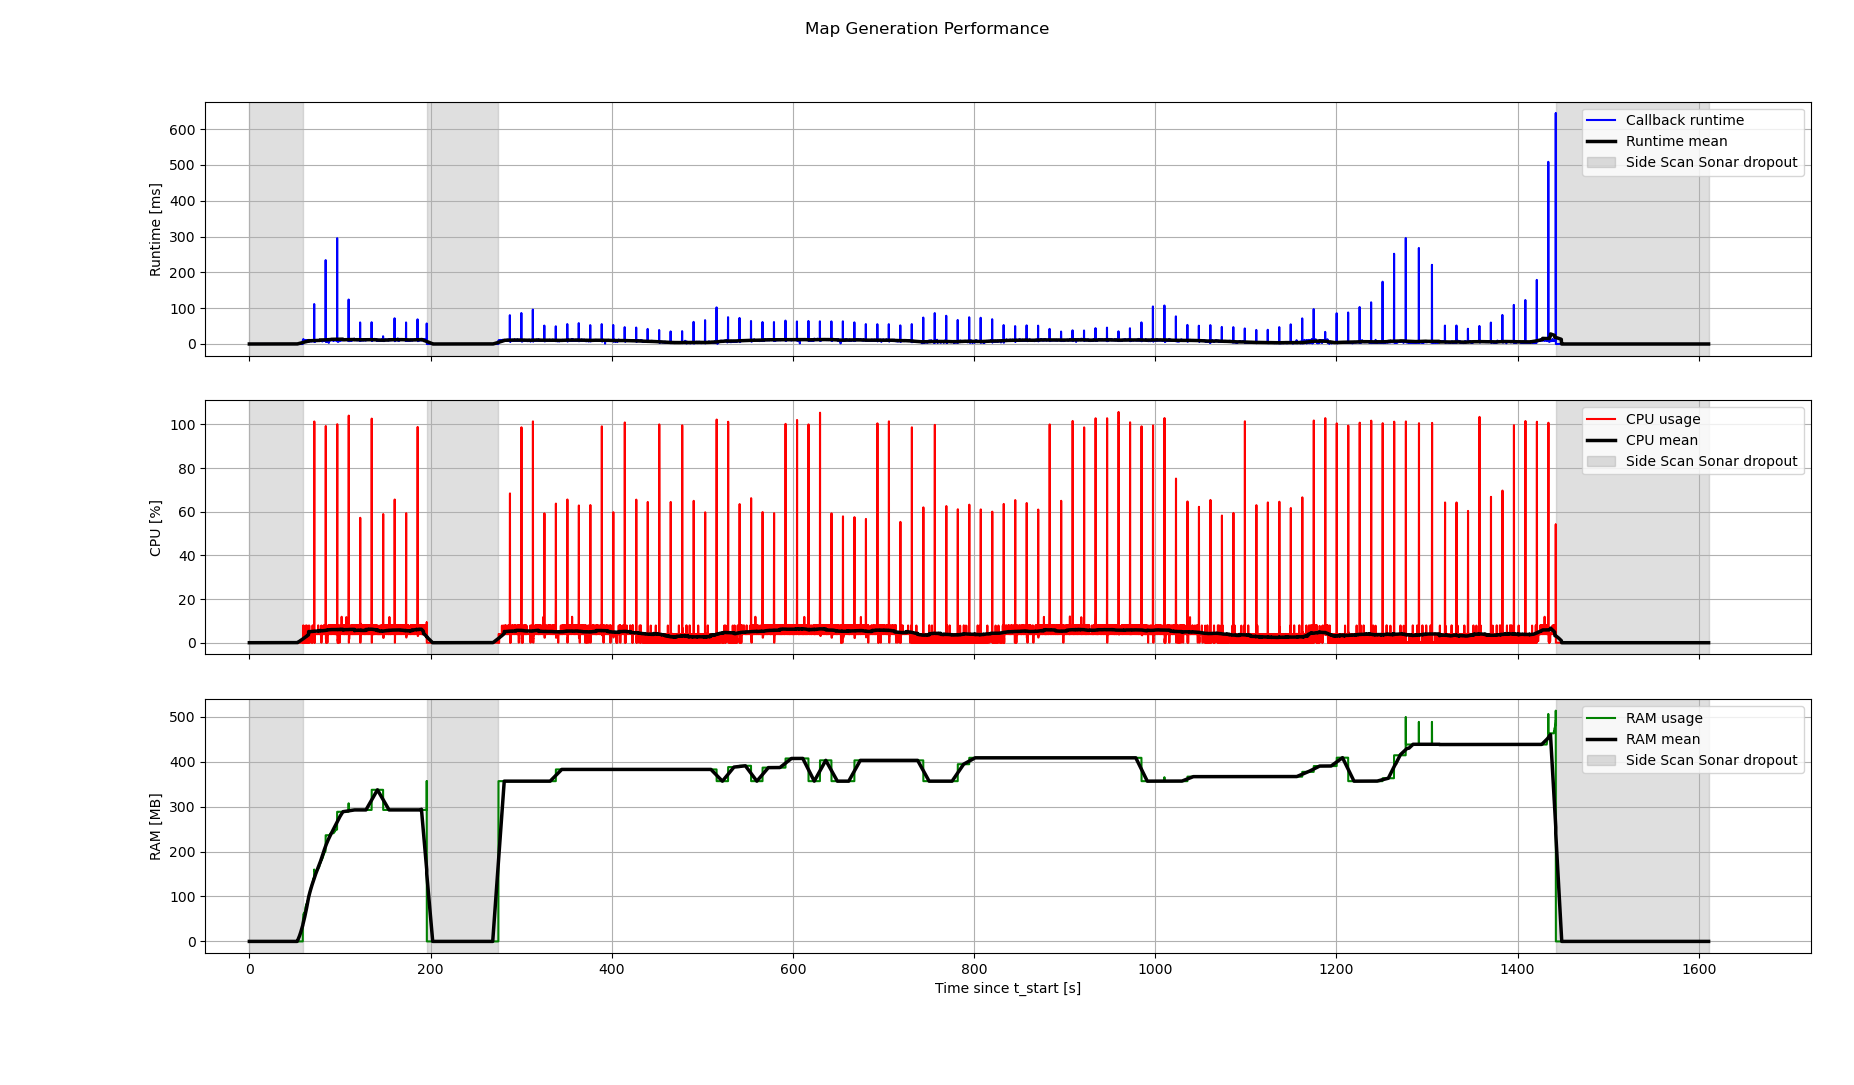
\includegraphics[width=1.00\linewidth]{Pictures/Results/Local_Map_Generation/Map_Generation/Performance.png}
    \caption{Runtime, CPU usage, and memory consumption of the local map generation stage using the default parameter set.}
    \label{fig:results-local-map-generation-map-generation-performance}
\end{figure}

\begin{table}[H]
    \centering
    \caption{Runtime summary for the local map generation stage using the default parameter set.}
    \label{tab:results-local-map-generation-map-generation-runtime-default}
    \begin{tabular}{l c c c}
        \hline
        Function/Stage & Calls & Average runtime [ms] & Peak runtime [ms] \\
        \hline
        Swath buffering and accumulation into map states & 10212 & 6.466 & 14.998 \\
        Dense map construction step & 105 & 51.052 & 208.027 \\
        \hline
    \end{tabular}
\end{table}
\noindent
Figure \ref{fig:results-local-map-generation-map-generation-performance} and Table \ref{tab:results-local-map-generation-map-generation-runtime-default} summarize the computational performance of the full local map generation stage using the default parameter set. Two parts of the implementation are especially relevant here. The first is the buffering step, where each processed swath is inserted into the persistent map states through candidate generation, pruning, interpolation, and accumulation. The second is the dense map construction step, where the accumulated sparse states are converted into the final local map image and then published.
\\ \\
The buffering step remains comparatively lightweight. Even though this stage contains the probabilistic pruning, backprojection, interpolation, and persistent accumulation logic, its average runtime is only about $6.5\,\mathrm{ms}$, with a peak below $15\,\mathrm{ms}$. This shows that the core probabilistic map generation itself is already efficient and is not the dominant bottleneck of the system. In practice, this part of the implementation is sufficiently lightweight to run comfortably on an embedded SBC.
\\ \\
The larger runtime peaks are mainly associated with the dense map construction and publication step. The average runtime of this step is about $51,\mathrm{ms}$, while the measured algorithmic peak is about $208,\mathrm{ms}$. This is consistent with the fact that this stage must traverse all active chunks, reconstruct the dense image, and run the local gap filling stage before the result is published. In the full runtime trace, however, the observed peaks reach up to about $600,\mathrm{ms}$, which shows that a substantial part of the total peak cost does not come from the map calculation alone, but from ROS2 publishing overhead. In other words, once the dense map has been constructed, a large additional cost is incurred by moving, copying, and transmitting the resulting image through the ROS2 communication layer. The main practical bottleneck is therefore not only the normalization and reconstruction itself, but also the memory movement and message passing required to handle a very large dense map output.
\\ \\
An important observation is that the runtime peaks correlate well with periods where the state estimate degrades, especially during dead reckoning. As discussed earlier in the state estimation results and in Figure \ref{fig:results-state-estimation-position}, when aiding is lost the accumulated pose error causes the reconstructed swaths to spread out more than they should. This leads directly to larger candidate regions, more active chunks, and a larger final dense map. As a result, both memory usage and runtime increase during these periods. In this sense, dead reckoning not only degrades map quality, but also increases the computational cost of the map generation stage.
\\ \\
Even under these more demanding conditions, however, the implementation remains real time in practice. The node continues to run smoothly without instability or dropped processing. This is important, because the largest peaks seen in the measured runtime are not purely algorithmic. A significant part of the peak cost comes from handling and publishing large map outputs through ROS2, which introduces additional overhead beyond the core map calculations themselves. Thus, although the plotted peaks can appear large, the underlying map generation algorithm remains computationally manageable and the overall system still behaves robustly in real operation.
\\ \\
From a tuning perspective, these results also indicate which parameters are most important for performance. The two pruning thresholds can reduce compute by making candidate support smaller, but in the present implementation the probabilistic stages are already relatively efficient. More important in practice are the parameters that control the size of the accumulated map state and the final dense image, such as the dense map update interval, retained active history through chunk aging, chunk size, and especially the map resolution. These parameters influence how much data must be stored, traversed, reconstructed, and published, which is why they have a particularly strong effect on the end to end runtime.

\newpage

\begin{figure}[H]
    \centering
    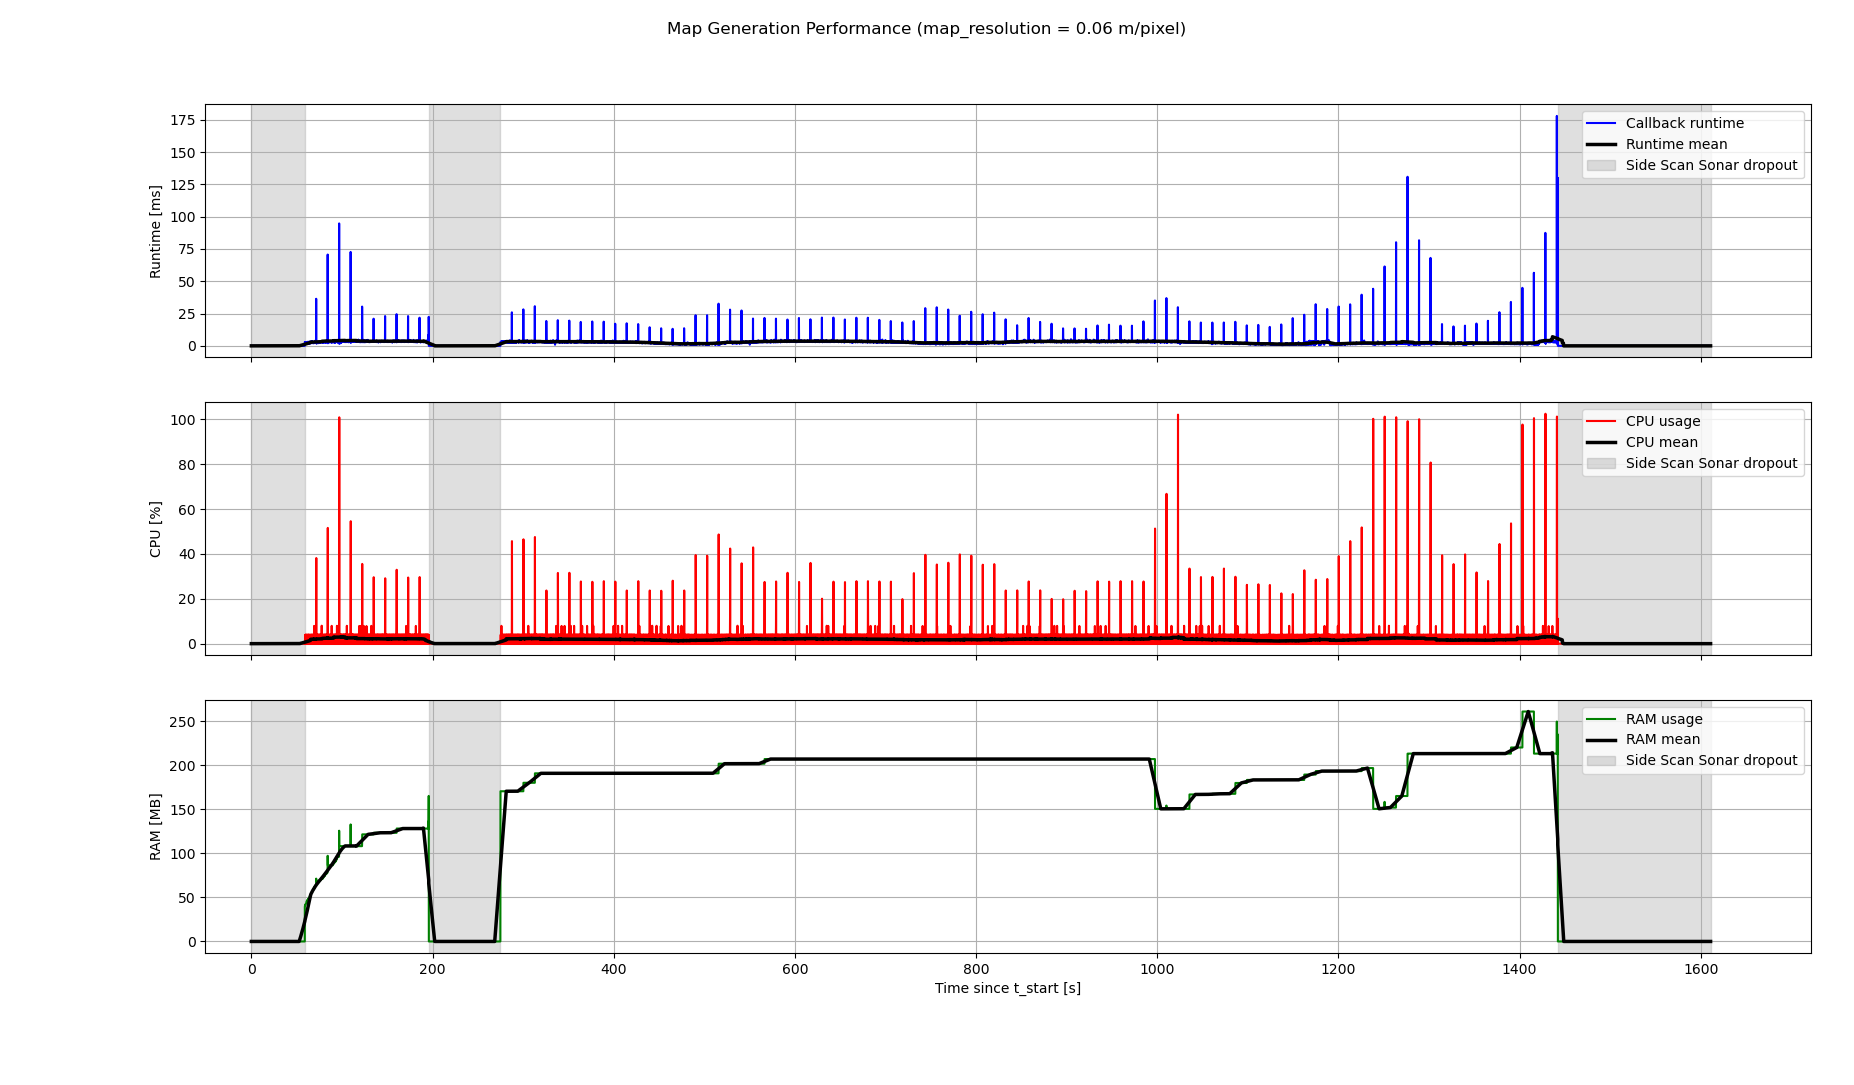
\includegraphics[width=1.00\linewidth]{Pictures/Results/Local_Map_Generation/Map_Generation/Performance_map_resolution_0.06.png}
    \caption{Runtime, CPU usage, and memory consumption of the local map generation stage when the map resolution is changed from $0.03$ to $0.06\,\mathrm{m/pixel}$.}
    \label{fig:results-local-map-generation-map-generation-performance-tuned}
\end{figure}
\begin{figure}[H]
    \centering
    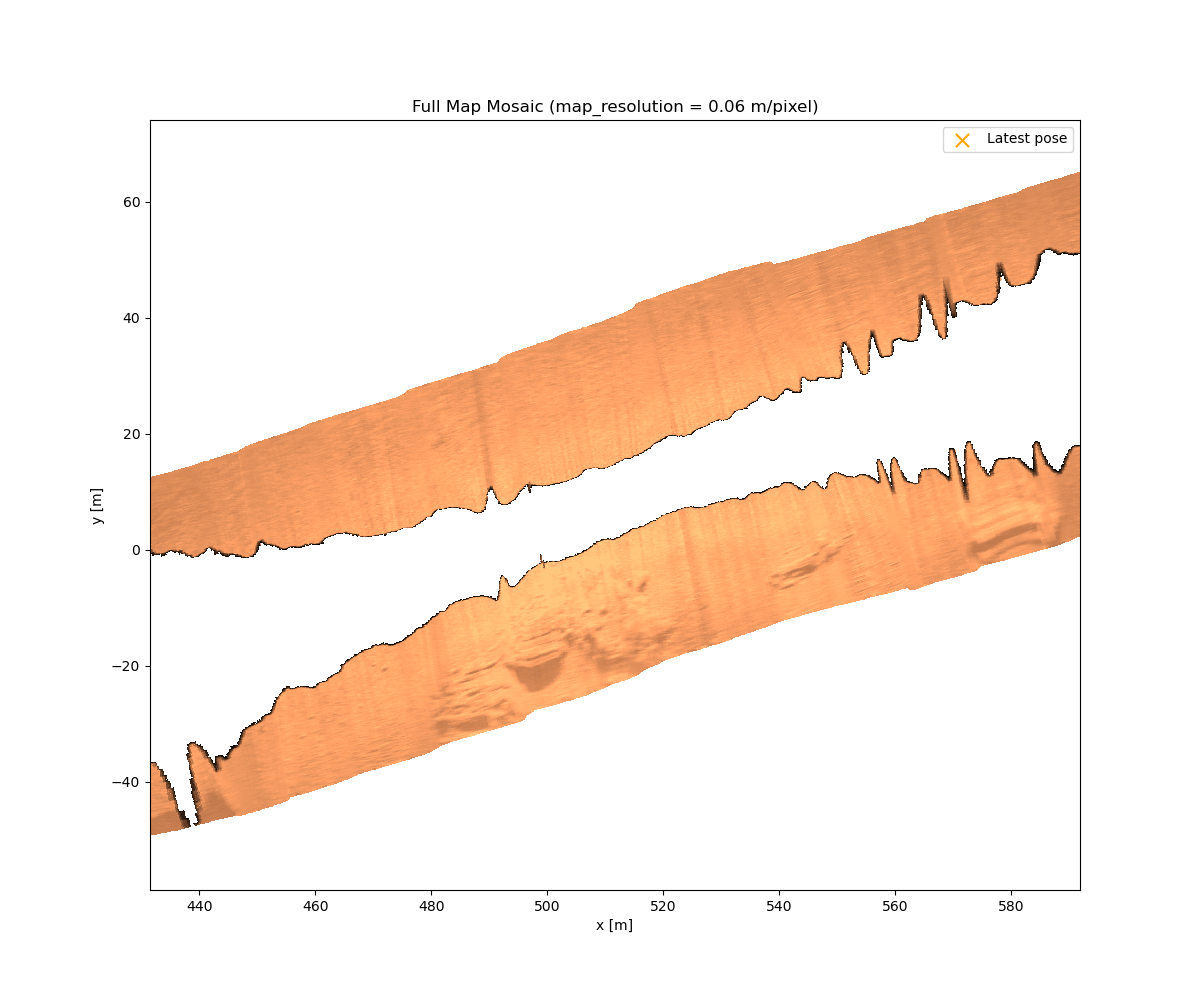
\includegraphics[width=0.85\linewidth]{Pictures/Results/Local_Map_Generation/Map_Generation/Full_Map_zoomed_in_map_resolution_0.06.png}
    \caption{Example local map result when the map resolution is changed from $0.03$ to $0.06\,\mathrm{m/pixel}$.}
    \label{fig:results-local-map-generation-map-generation-map-resolution-tuned}
\end{figure}

\newpage

\begin{table}[H]
    \centering
    \caption{Runtime summary for the local map generation stage when only the map resolution is changed to $0.06\,\mathrm{m/pixel}$.}
    \label{tab:results-local-map-generation-map-generation-runtime-tuned}
    \begin{tabular}{l c c c}
        \hline
        Function/Stage & Calls & Average runtime [ms] & Peak runtime [ms] \\
        \hline
        Swath buffering and accumulation into map states & 10212 & 1.647 & 7.034 \\
        Dense map construction step & 105 & 20.636 & 85.008 \\
        \hline
    \end{tabular}
\end{table}
\noindent
To examine the sensitivity of the implementation to parameter tuning, an additional run was performed where all parameters were kept unchanged except for the map resolution, which was increased from $0.03$ to $0.06\,\mathrm{m/pixel}$. The corresponding performance results are shown in Figure \ref{fig:results-local-map-generation-map-generation-performance-tuned} and Table \ref{tab:results-local-map-generation-map-generation-runtime-tuned}, while an example of the resulting map output is shown in Figure \ref{fig:results-local-map-generation-map-generation-map-resolution-tuned}.
\\ \\
This parameter change has a very strong effect on runtime. The average buffering runtime decreases from about $6.5\,\mathrm{ms}$ to about $1.6\,\mathrm{ms}$, and the average dense map construction runtime decreases from about $51\,\mathrm{ms}$ to about $20.6\,\mathrm{ms}$. The peak runtimes are also reduced substantially. This confirms that the map resolution is the single most influential parameter for the practical computational cost of the map generator. The reason is straightforward, a coarser map produces fewer cells overall, which means fewer candidate insertions, fewer active pixels, less persistent map data, less fill in work, and less memory movement when the dense image is rebuilt and published.
\\ \\
This reduction is especially important because the dominant cost of the full pipeline is strongly tied to data volume. Once the dense map becomes large, the system must not only compute over more pixels, but also move more memory and publish larger messages. Reducing the map resolution therefore improves performance in several ways at once. It reduces the size of the persistent states, reduces the cost of dense map construction, reduces local gap filling work, and reduces the amount of image data that must be transported through the system. In practice, this kind of reduction often gives a larger performance benefit than tuning the probabilistic thresholds alone.
\\ \\
At the same time, Figure \ref{fig:results-local-map-generation-map-generation-map-resolution-tuned} shows that the resulting map remains visually very similar to the default case. The main seabed features are still clearly visible, and with the naked eye the loss in quality is relatively small. This means that moderate downscaling of the map resolution can be a very effective practical choice when compute resources are limited. For later feature extraction, such a map can still remain fully useful even though it no longer matches the raw sonar sample spacing exactly.
\\ \\
This does not mean that the map resolution can be reduced arbitrarily. If it is downscaled too aggressively, for example by an order of magnitude or more, then useful spatial detail will eventually be compressed away and the map may lose information important for later feature extraction and matching. Thus, the map resolution should be understood as a tuning parameter that balances computational cost against retained spatial detail.
\\ \\
In the present work, the default resolution of $0.03\,\mathrm{m/pixel}$ was kept because it already runs in real time on the target embedded platform while preserving more detail. The additional $0.06\,\mathrm{m/pixel}$ experiment is therefore not introduced because the default setting was insufficient, but rather to illustrate how strongly performance can be improved when needed by changing a single parameter. This also demonstrates that the implemented map generation stage is flexible and can be adapted relatively easily to different vehicles and compute budgets. For lower end embedded systems, meaningful runtime reductions can be achieved simply by tuning a small set of parameters, with map resolution being the most influential of them.



\newpage



\subsubsection{Feature Extarction}
\paragraph{Map Filtering} \mbox{}\\[0.5em] \noindent
The first step in the feature extraction stage is to filter the normalized local map before segmentation. The purpose of this step is to reduce small scale speckle noise and unstable intensity variations while preserving the sharp transitions that define echo and shadow boundaries. This is important because the later segmentation stage depends directly on these local intensity structures.
\begin{figure}[H]
    \centering
    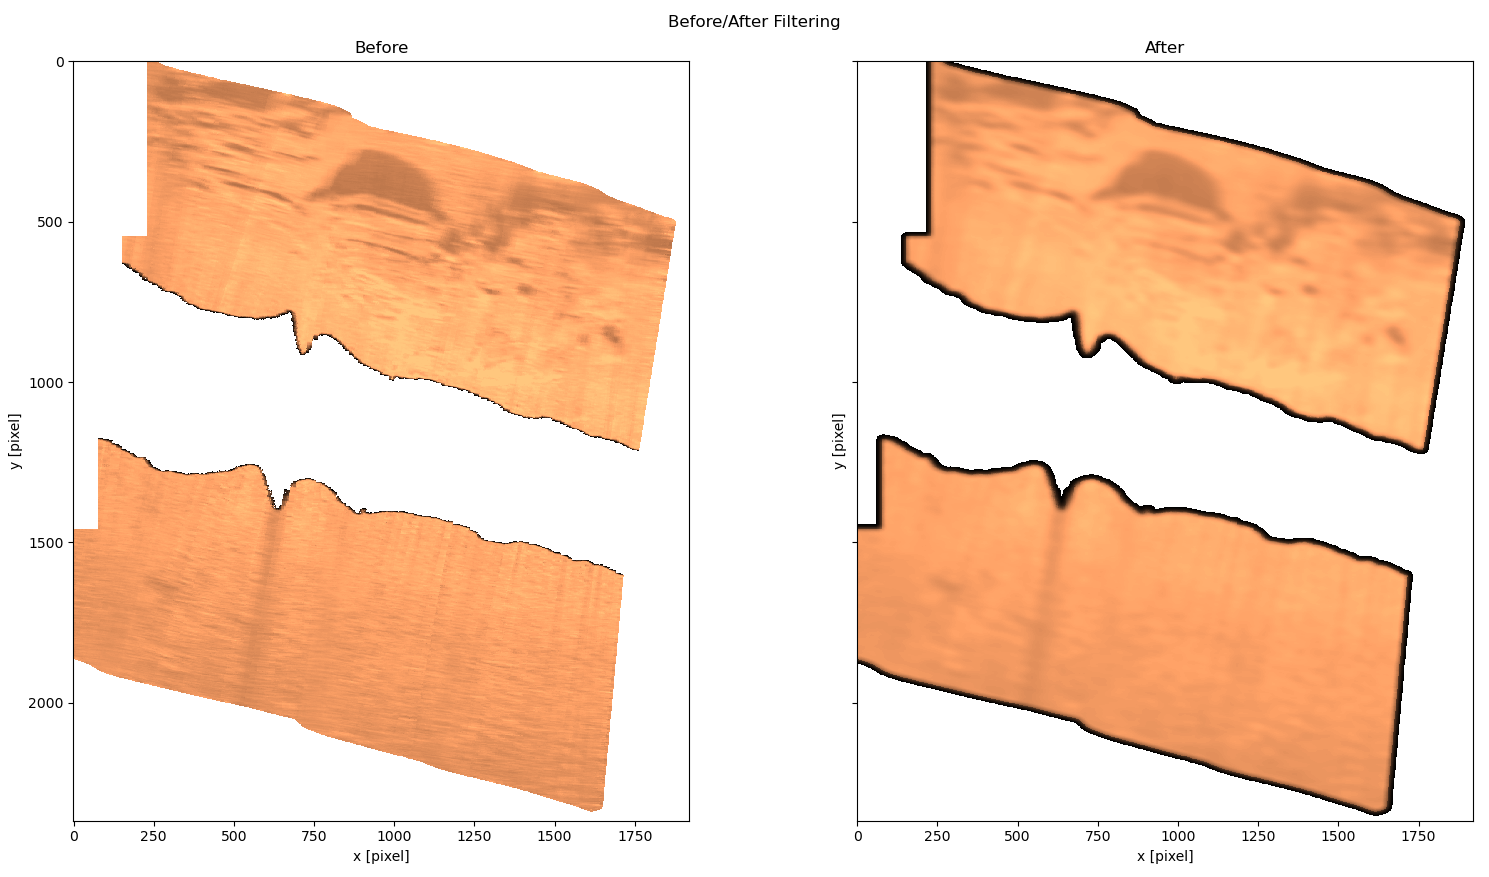
\includegraphics[width=0.95\linewidth]{Pictures/Results/Local_Map_Generation/Feature_Extraction/Filter_zoomed_out.png}
    
    \vspace{0.5em}
    
    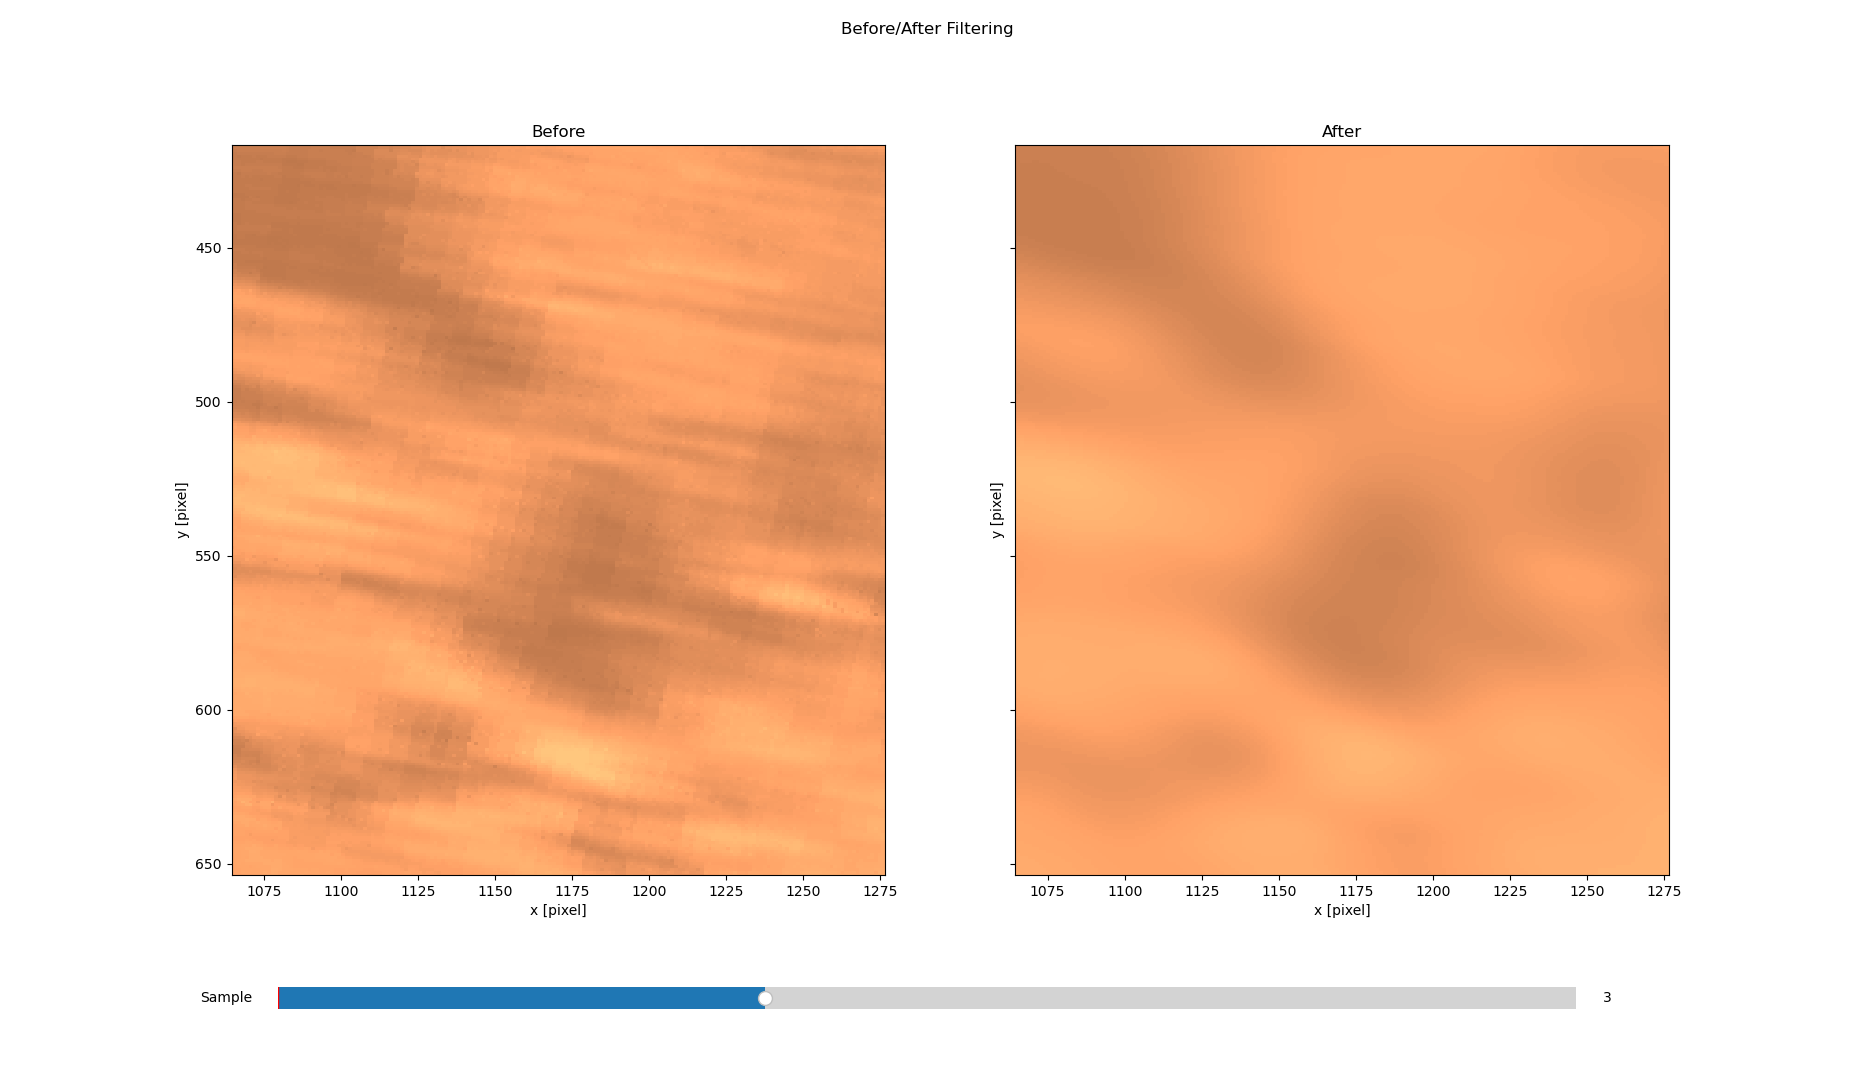
\includegraphics[width=0.95\linewidth]{Pictures/Results/Local_Map_Generation/Feature_Extraction/Filter_zoomed_in.png}
    \caption{Effect of edge preserving filtering on the normalized local map. The zoomed out view shows that the main map structure is preserved, while the zoomed in view shows the smoothing effect more clearly. Small speckle artifacts are reduced and local intensity transitions become smoother, while important echo and shadow boundaries remain sharp enough for later segmentation.}
    \label{fig:results-local-map-generation-feature-extraction-filter}
\end{figure}

\newpage

\noindent
Figure \ref{fig:results-local-map-generation-feature-extraction-filter} shows the effect of the edge preserving filter. In the zoomed out view, the difference between the original and filtered map is not very large, since the main seabed structures and global intensity pattern are preserved. In the zoomed in view, however, the effect is much clearer. Small speckle artefacts are smoothed away, and local intensity transitions become more continuous, while the main feature boundaries remain visible.
\\ \\
This behavior is important for feature extraction. A simple Gaussian filter would also reduce speckle noise, but it would blur object boundaries and make echo-shadow transitions less distinct from the surrounding background. That would make it harder for the segmentation stage to determine where a feature starts and ends. The bilateral filter is therefore more useful here, even though it is slightly more expensive computationally, because it improves local stability without destroying the edge information needed for landmark detection.
\\ \\
Overall, the filtered result provides a cleaner and more stable input for semantic segmentation. The added filtering cost is justified because better preserved boundaries and reduced noise lead to more reliable candidate regions in the following stages.

\newpage

\paragraph{Semantic Segmentation} \mbox{}\\[0.5em] \noindent
\begin{figure}[H]
    \centering
    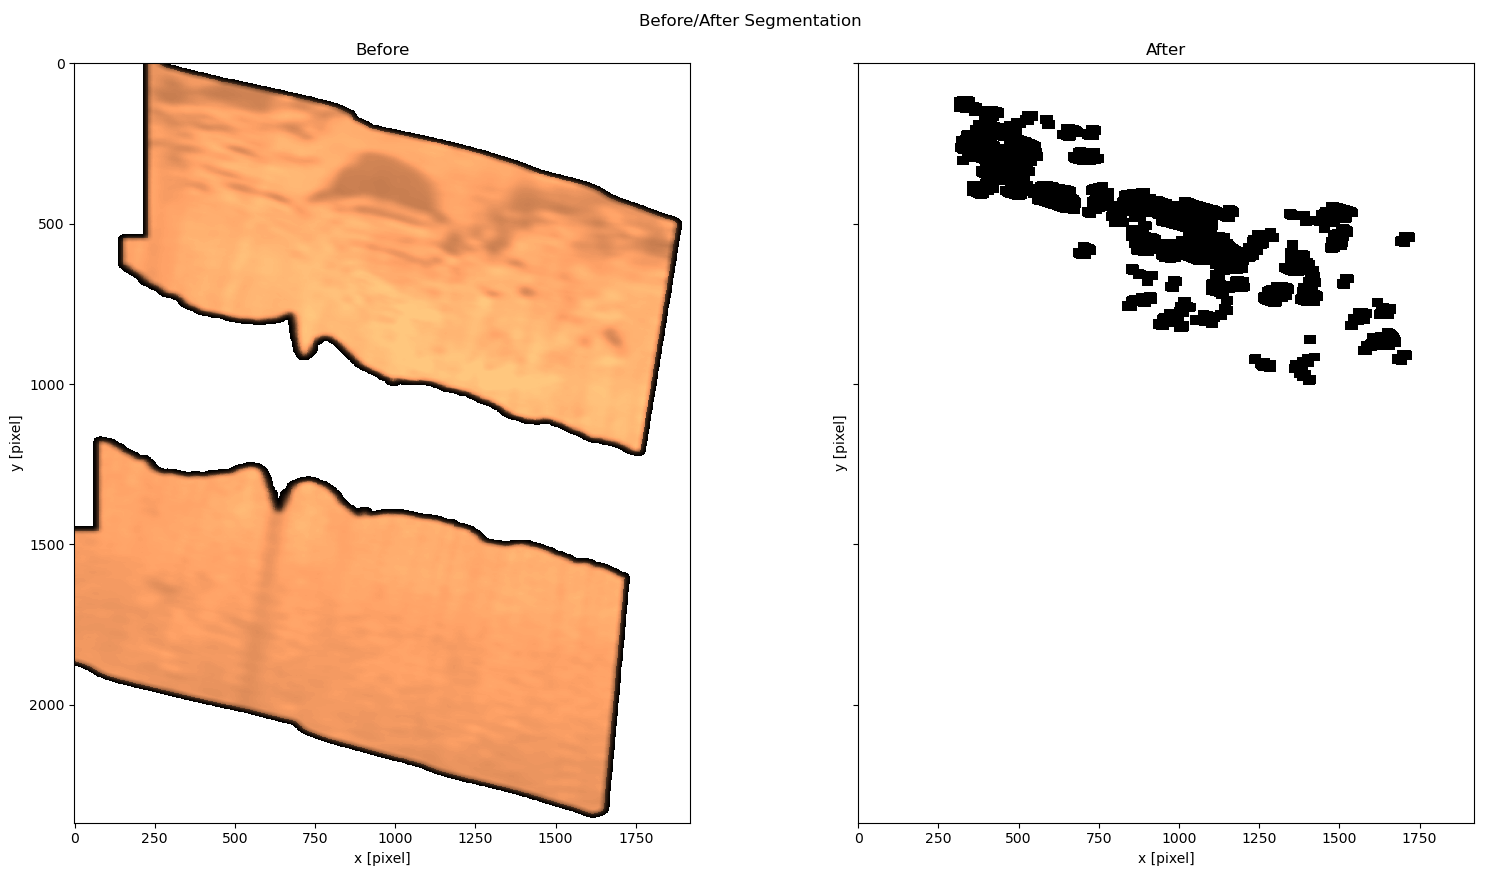
\includegraphics[width=0.85\linewidth]{Pictures/Results/Local_Map_Generation/Feature_Extraction/Segmentation.png}
    \caption{Result of semantic segmentation applied to the filtered local map. The method extracts candidate landmark regions by using the echo-shadow relationship as prior information, rather than relying only on local intensity thresholds. This allows object-like sonar structures to be separated more reliably from background texture while remaining lightweight enough for real-time processing.}
    \label{fig:results-local-map-generation-feature-extraction-segmentation}
\end{figure}
\noindent
After filtering, the local map is segmented to separate candidate landmark regions from the surrounding background. This is the first stage where acoustic features are explicitly extracted from the map. Instead of relying only on classical thresholding or edge detection, the segmentation uses the semantic echo-shadow relationship of side scan sonar imagery. Regions that contain both a bright acoustic response and nearby dark shadow support are treated as more likely landmark candidates.
\\ \\
Figure \ref{fig:results-local-map-generation-feature-extraction-segmentation} shows the result of this semantic segmentation stage. The method succeeds in extracting the main object-like structures while avoiding many background regions that would otherwise be difficult to reject using only intensity thresholds. This is important because the normalized map can still contain darker and brighter seabed texture that does not correspond to physical landmarks. Even adaptive thresholding can struggle in these cases, since local intensity changes may come from illumination variation, seabed texture, or shadowed objects, and these can be difficult to separate from intensity alone.
\\ \\
The semantic approach is therefore a useful compromise between classical image processing and full ML based segmentation. Classical methods would be faster, but are more likely to segment incorrect regions in complex sonar imagery, witch would introduce false landmarks in later DA step in SLAM. ML based methods could potentially be more accurate, but require labelled training data and significantly higher computational cost. The method used here instead applies simple prior knowledge about sonar shadows, which is general enough to work across side scan sonar maps while still remaining suitable for real-time operation on constrained hardware.
\\ \\
Some small artifacts remain after segmentation, which is expected as the method is not perfect. The purpose of this stage is not to produce the final landmark set directly, but to generate a meaningful candidate mask. Small noisy regions and unstable fragments are handled in the following labelling stages.

\newpage

\paragraph{Labelling} \mbox{}\\[0.5em] \noindent
\begin{figure}[H]
    \centering
    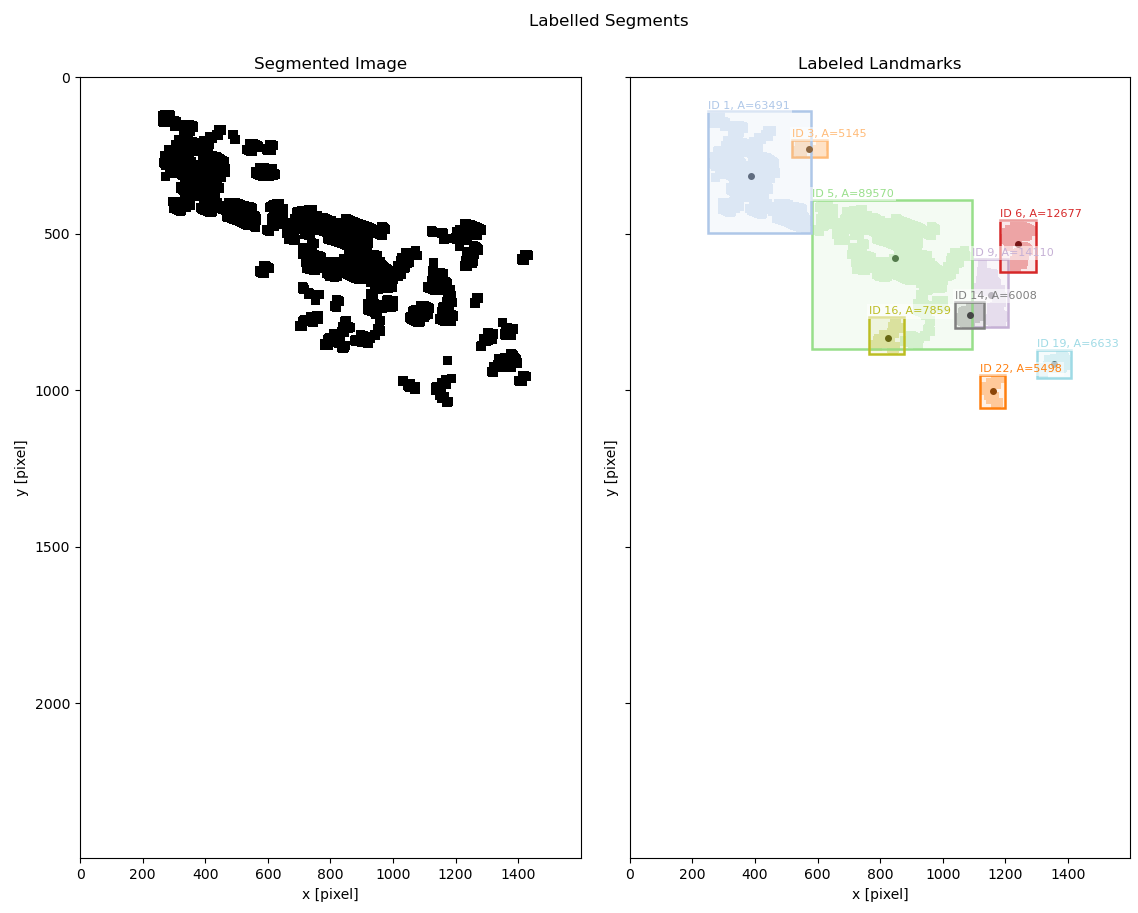
\includegraphics[width=0.95\linewidth]{Pictures/Results/Local_Map_Generation/Feature_Extraction/Labelling.png}
    \caption{Connected component labelling of the segmented candidate mask. Each coherent region is assigned a unique label, allowing landmark candidates to be separated and analyzed individually. Small segmented regions are pruned using a minimum area threshold, reducing weak artifacts and ensuring that only stronger and more coherent landmark candidates are passed further into the pipeline.}
    \label{fig:results-local-map-generation-feature-extraction-labelling}
\end{figure}
\noindent
After segmentation, the candidate mask is processed using connected component labelling. Each coherent segmented region is assigned a unique label, allowing the individual landmark candidates to be separated and analyzed independently. During this step, useful geometric information such as the bounding box, region area, and centroid can also be extracted directly from the labelled regions, which avoids repeating the same image scans later in the pipeline.
\\ \\
Figure \ref{fig:results-local-map-generation-feature-extraction-labelling} shows the labelled candidate regions after segmentation. The main object-like structures are preserved as separate components, while smaller isolated regions are removed by the minimum area threshold. This pruning is important because very small segmented blobs are often caused by residual speckle, weak texture variation, or fragmented segmentation artifacts rather than stable acoustic landmarks.
\\ \\
The minimum area criterion is therefore used as a conservative quality filter. Some small regions may represent real weak features, but keeping all of them would increase the number of false landmarks passed to data association. This would slow down matching and increase the risk of incorrect associations in SLAM. It is therefore preferable to reject uncertain small candidates early and only pass stronger, coherent regions further into the feature extraction pipeline.

\newpage

\paragraph{Landmark Measurements} \mbox{}\\[0.5em] \noindent
\begin{figure}[H]
    \centering
    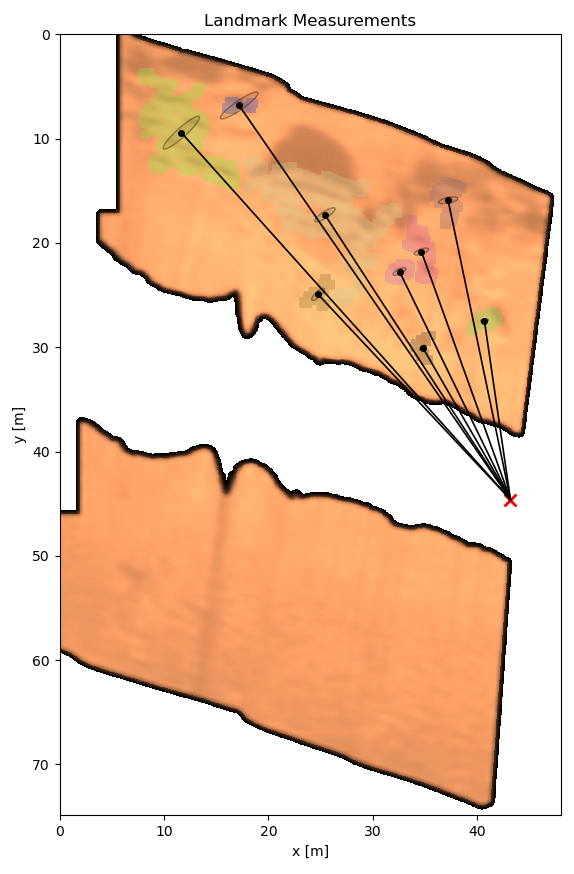
\includegraphics[width=0.60\linewidth]{Pictures/Results/Local_Map_Generation/Feature_Extraction/Landmark_Measurements.png}
    \caption{Detected landmark regions and corresponding range-bearing measurements overlaid on the local reflectivity map. The vehicle pose is shown in the local map frame, and each landmark measurement connects the vehicle to the landmark centroid. The associated uncertainty increases with landmark range, giving closer landmarks higher confidence than distant landmarks.}
    \label{fig:results-local-map-generation-feature-extraction-landmark-measurements}
\end{figure}
\noindent
After labelling and pruning, each remaining landmark candidate is converted into a SLAM measurement relative to the vehicle pose in the local map. Figure \ref{fig:results-local-map-generation-feature-extraction-landmark-measurements} shows the local reflectivity map with the vehicle pose, detected landmark regions, and the corresponding range-bearing measurements overlaid. The measurement line connects the vehicle frame to each landmark centroid, while the plotted uncertainty indicates the confidence assigned to that observation.
\\ \\
The result illustrates the expected range dependent uncertainty behavior used by the landmark measurement model. In this local map representation, the landmarks are not observed from a single image snapshot, but from a map constructed by accumulating many sonar swaths along the vehicle trajectory. Therefore, the increased uncertainty is not mainly caused by image resolution alone. It is primarily caused by the relative measurement geometry between the current vehicle pose and the landmark. As the vehicle moves farther from a landmark, the range-bearing measurement becomes more sensitive to pose error, heading error, and viewing angle. Distant landmarks are therefore assigned larger uncertainty, while nearby landmarks are treated as more reliable for the current SLAM update.

\newpage

\paragraph{Landmark Height Estimation} \mbox{}\\[0.5em] \noindent
\begin{figure}[H]
    \centering
    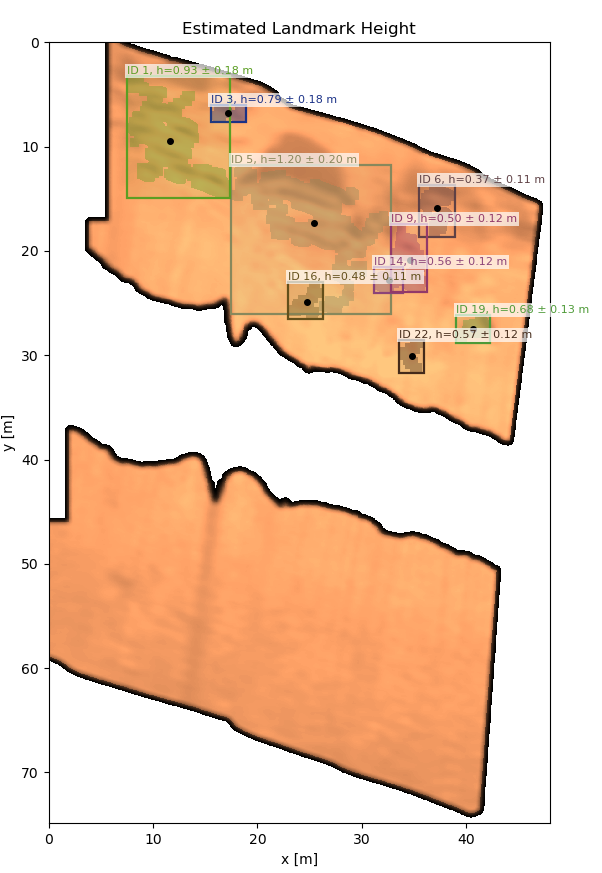
\includegraphics[width=0.60\linewidth]{Pictures/Results/Local_Map_Generation/Feature_Extraction/Estimated_Height.png}
    \caption{Estimated landmark heights and corresponding uncertainty values. Landmarks with longer acoustic shadows generally produce larger height estimates. Landmarks with similar distance geometry can have similar uncertainty, while differences in shadow length still lead to different estimated heights.}
    \label{fig:results-local-map-generation-feature-extraction-height}
\end{figure}
\noindent
After the landmark regions have been detected, an approximate height is estimated from the associated acoustic shadow geometry. Figure \ref{fig:results-local-map-generation-feature-extraction-height} shows the estimated height values for the detected landmarks together with their corresponding uncertainty. The result follows the expected behavior, landmarks with longer acoustic shadows generally receive larger height estimates, since a taller structure blocks the sonar beam over a longer distance.
\\ \\
The figure also shows that landmarks at similar ground distance from the sonar swath can still receive different height estimates when their shadow lengths differ. This is consistent with the shadow based height model, where both the shadow length and the sonar to landmark geometry influence the final estimate. The uncertainty follows the same principle, it depends on the estimated height, the shadow length, and the distance geometry. Landmarks with similar viewing geometry can therefore have similar uncertainty even when their estimated heights differ.
\\ \\
These results should be interpreted as approximate geometric cues rather than precise object height measurements. The estimate depends on correct shadow association and on the simplified flat-ground shadow model, but it still provides useful additional structure information about the detected landmarks.

\newpage

\paragraph{Landmark Descriptors} \mbox{}\\[0.5em] \noindent
\begin{figure}[H]
    \centering
    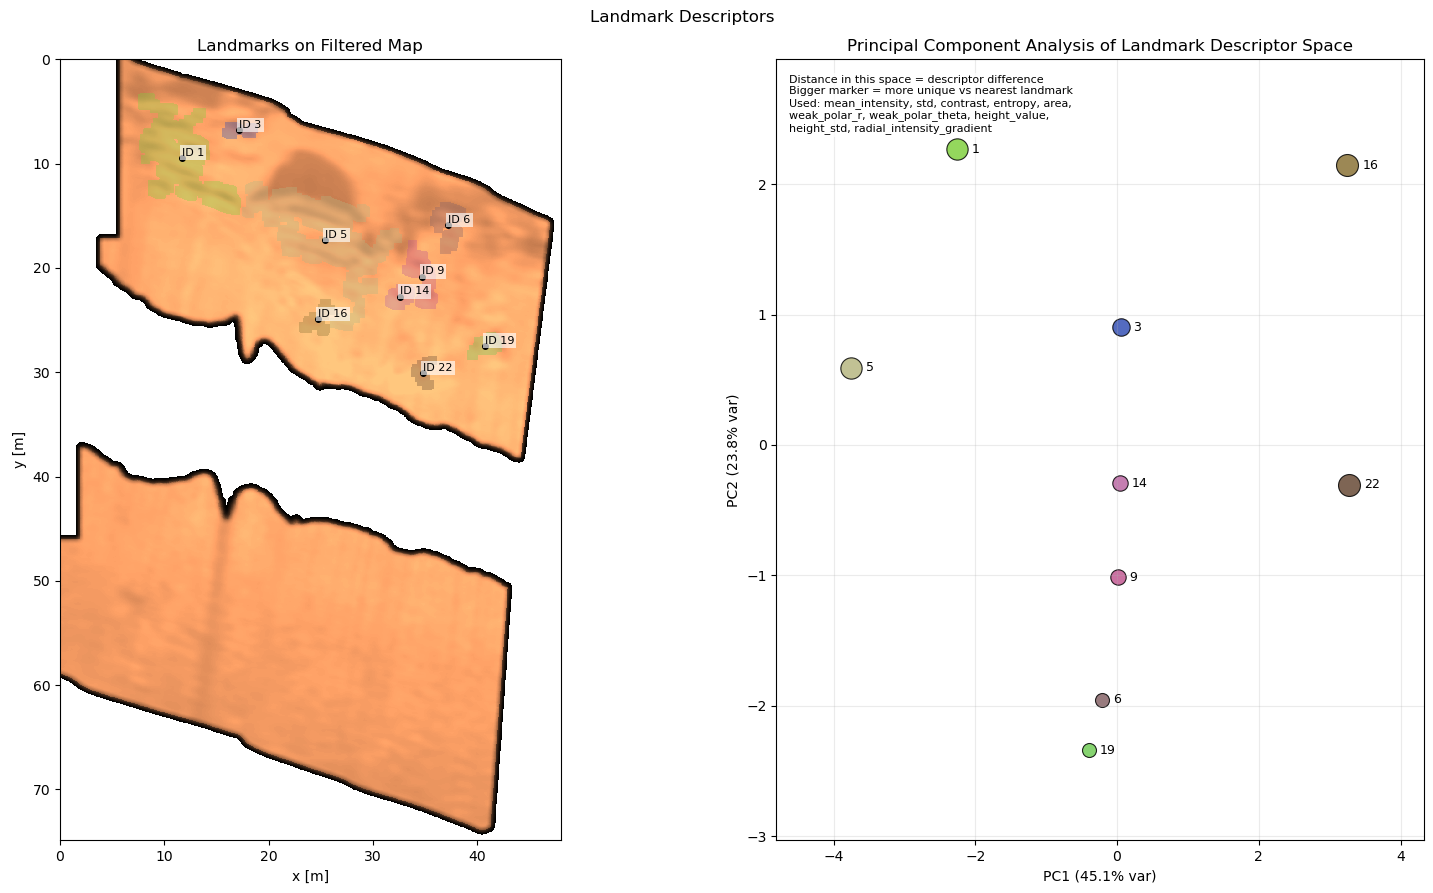
\includegraphics[width=0.95\linewidth]{Pictures/Results/Local_Map_Generation/Feature_Extraction/Descriptors.png}
    \caption{PCA visualization of the landmark descriptor vectors. Each point represents one detected landmark projected from the full descriptor space into two principal components. The plot gives a qualitative view of descriptor separability, but does not show the complete high dimensional matching space. The descriptors act as compact landmark fingerprints, allowing fast candidate pruning before more expensive geometric data association is performed.}
    \label{fig:results-local-map-generation-feature-extraction-descriptors}
\end{figure}
\noindent
After landmark measurement and height estimation, each landmark is assigned a compact descriptor vector containing the most important appearance, geometric, and uncertainty related information about the landmark. Since the full descriptor is higher dimensional and difficult to visualize directly, Figure \ref{fig:results-local-map-generation-feature-extraction-descriptors} shows a two dimensional PCA (Principal Component Analysis) projection of the descriptor space. Each point represents one detected landmark descriptor, with the label corresponding to the landmark ID shown on the filtered map. The point position indicates descriptor similarity in the reduced PCA space, while the marker size represents the distance to the nearest neighbouring descriptor in the full descriptor space. Larger markers therefore indicate more unique landmarks, while smaller markers indicate landmarks that are more similar to another detected feature. Since PCA only preserves the two strongest directions of variation, the plot should be interpreted as a qualitative visualization of descriptor separability rather than the exact matching space used during data association.
\\ \\
The main motivation for using descriptors is computational efficiency. Directly comparing full landmark image regions, bounding boxes, or complete map patches would require comparing thousands of pixel values for each candidate match. This quickly becomes too expensive when data association must search through many landmarks and possible loop closure candidates. Instead, the descriptor compresses the landmark into a small feature vector that captures the most useful information for fast comparison. This acts like a compact fingerprint of the landmark.
\\ \\
This compression is not meant to replace the later geometric data association step. The descriptor is mainly used for fast candidate pruning, clearly different landmarks can be rejected quickly, while only plausible matches are passed on to more expensive and accurate association methods. This makes global lookup and loop closure proposal much faster, since the system compares compact descriptor vectors instead of large image regions. The strong descriptor terms provide appearance based discrimination, while the weak descriptor terms add supporting geometric and physical cues. Together, they provide a practical balance between compactness, distinctiveness, and real-time performance.

\newpage

\paragraph{Full Landmark Map} \mbox{}\\[0.5em] \noindent
\begin{figure}[H]
    \centering
    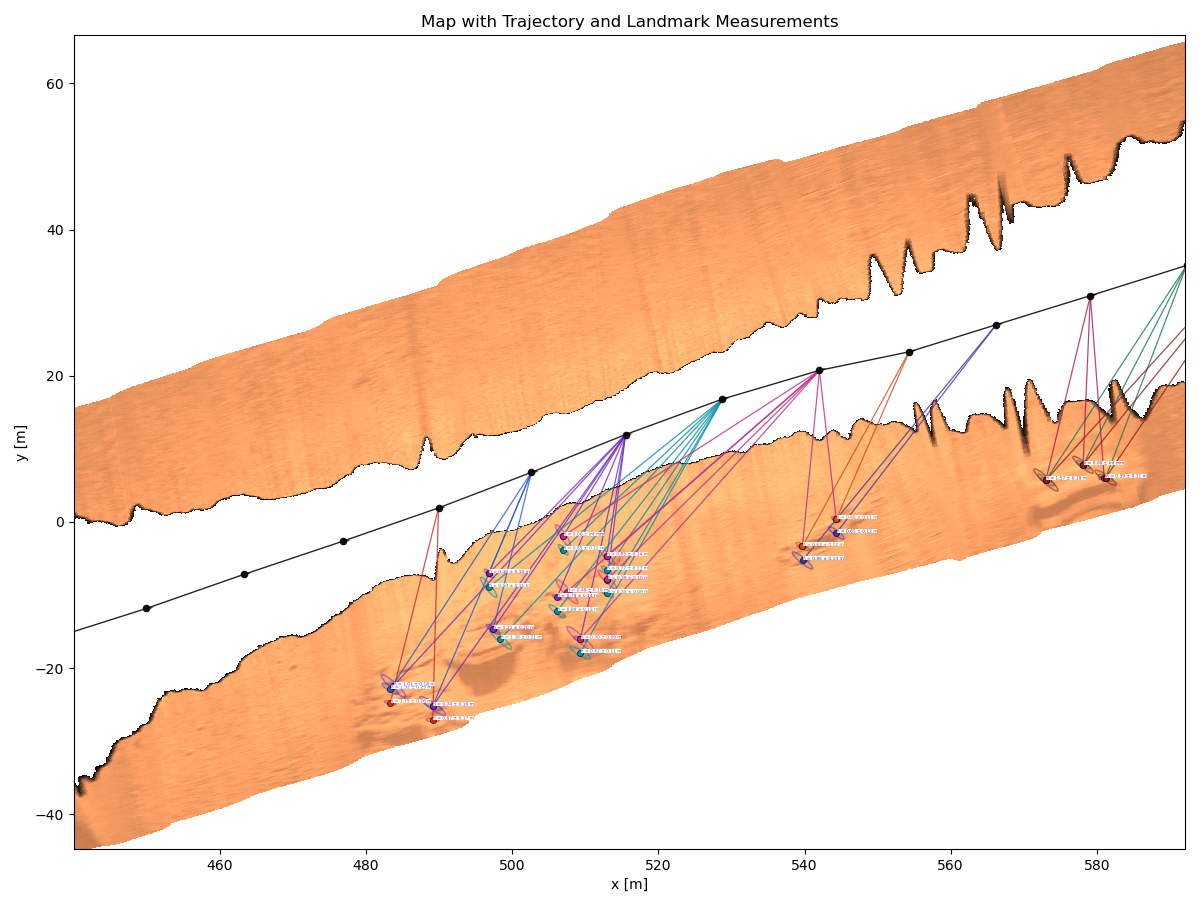
\includegraphics[width=0.70\linewidth]{Pictures/Results/Local_Map_Generation/Feature_Extraction/Full_Landmark_Measurements_zoomed_out.png}
    
    \vspace{0.5em}
    
    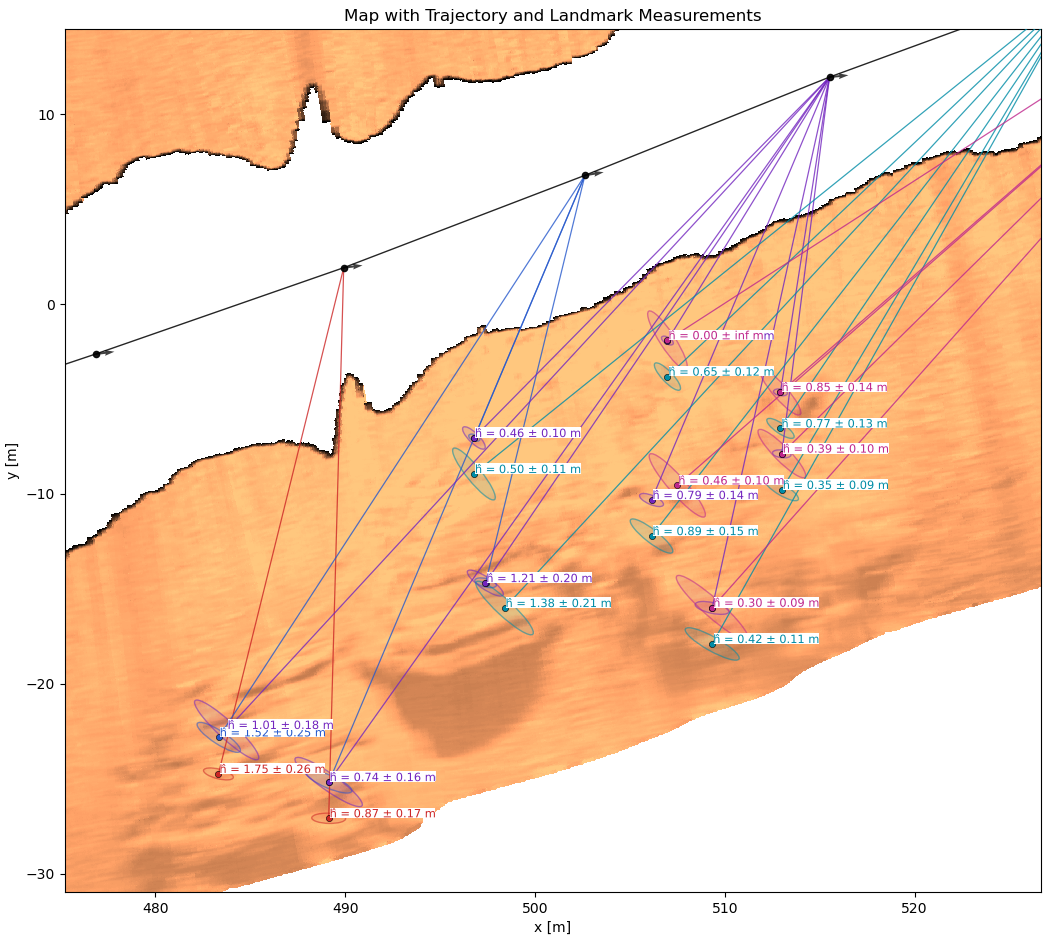
\includegraphics[width=0.70\linewidth]{Pictures/Results/Local_Map_Generation/Feature_Extraction/Full_Landmark_Measurements_zoomed_in.png}
    \caption{Global landmark map reconstructed from landmarks extracted in multiple overlapping local maps. The zoomed out view shows the overall spatial distribution of the detected landmarks, while the zoomed in view highlights that repeated detections of the same physical structures align consistently across local maps. The figure also shows that landmark height estimates remain reasonably stable, while more uncertain observations correctly receive larger associated variance.}
    \label{fig:results-local-map-generation-feature-extraction-full-landmark-map}
\end{figure}

\newpage

\noindent
To evaluate whether landmarks are detected consistently across time, the landmarks extracted from many overlapping local maps are projected into a common global frame and visualized together. Figure \ref{fig:results-local-map-generation-feature-extraction-full-landmark-map} shows this reconstructed global landmark map at two spatial scales. The main observation is that the same physical structures are repeatedly detected at consistent locations across multiple local maps, indicating that the feature extraction pipeline is stable and repeatable. This is especially visible in the zoomed in view, where multiple detections align well and preserve the overall spatial structure of the environment.
\\ \\
The figure also shows that the estimated landmark heights remain reasonably consistent across repeated detections of the same feature. Some repeated observations produce slightly different height values, but these differences are typically accompanied by larger uncertainty. This is expected, since landmarks observed from farther away or under less favorable viewing geometry are harder to estimate precisely. The associated height variance therefore increases in these cases, which correctly reflects the lower confidence in the estimate.
\\ \\
Overall, the result indicates that the full pipeline is able to extract stable landmark measurements and associated properties consistently across multiple local maps. This is important for SLAM in global feature matching and loop closure detection, since repeated observations of the same physical landmark should remain both spatially coherent and descriptively similar over time.

\newpage

\paragraph{Full Landmark Descriptors Map} \mbox{}\\[0.5em] \noindent
\begin{figure}[H]
    \centering
    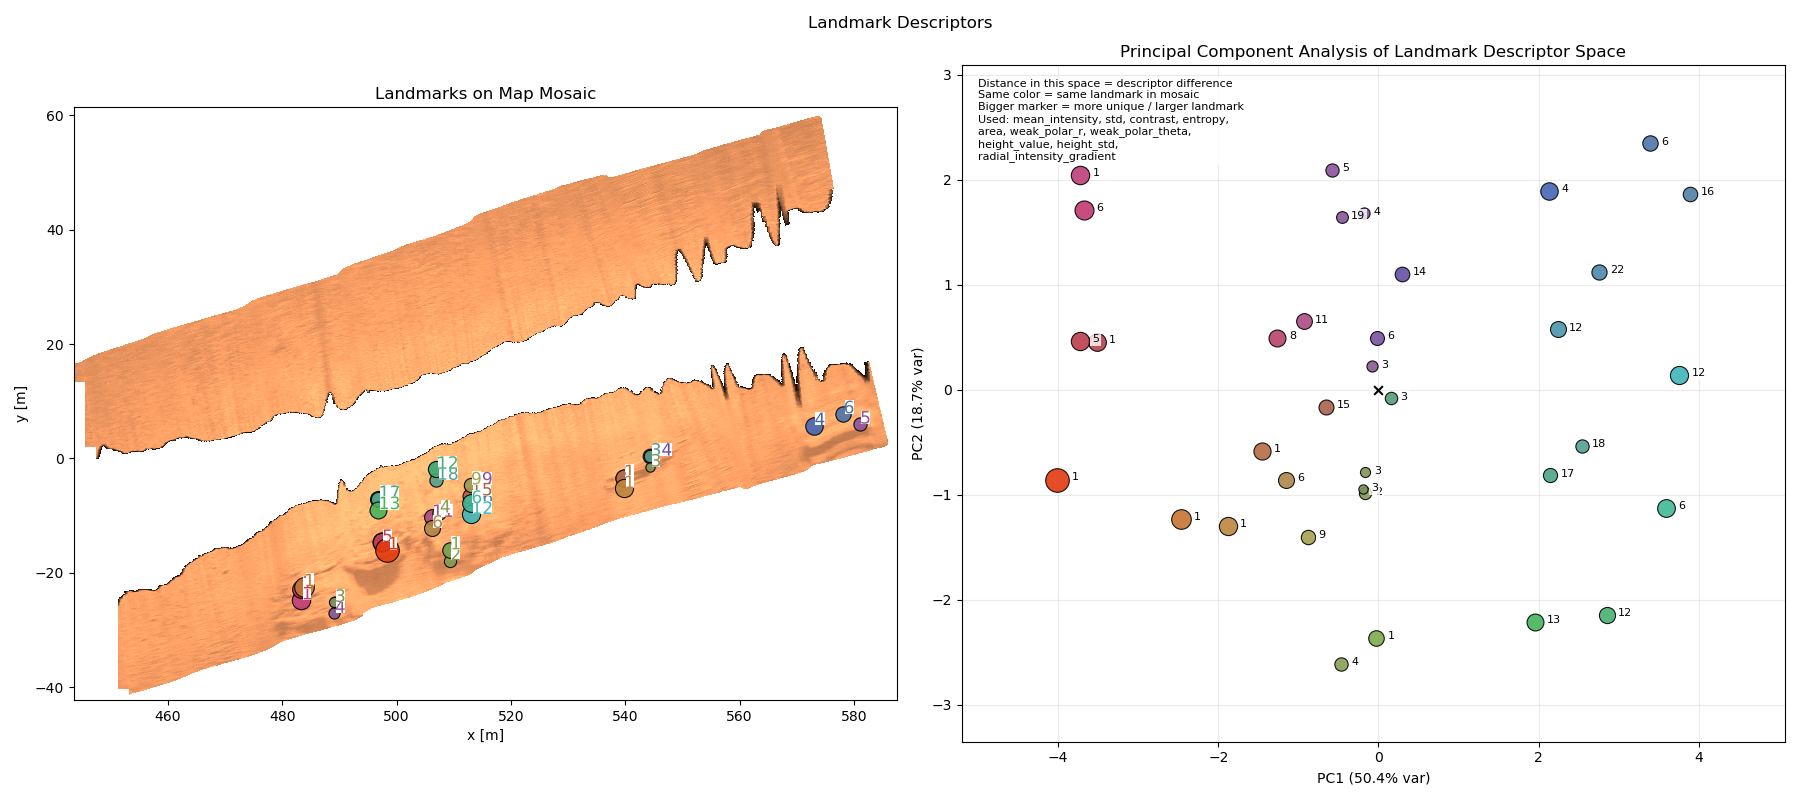
\includegraphics[width=0.95\linewidth]{Pictures/Results/Local_Map_Generation/Feature_Extraction/Full_Descriptors.png}
    \caption{Global landmark descriptor map. Each landmark is shown in the global frame and colored according to its location in the PCA projected descriptor space, with labels indicating landmark IDs. Similar colors indicate landmarks with more similar descriptors, while stronger color intensity and larger marker size indicate more unique landmarks relative to their nearest neighboring descriptor. The result illustrates that the descriptor representation provides a compact and useful fingerprint for fast landmark comparison and pruning during later data association.}
    \label{fig:results-local-map-generation-feature-extraction-full-descriptor-map}
\end{figure}
\noindent
To further evaluate descriptor consistency over the full mission, the descriptor information from all extracted landmarks is projected back into the global landmark map. Figure \ref{fig:results-local-map-generation-feature-extraction-full-descriptor-map} shows this result, where each landmark is assigned a color based on its location in the PCA descriptor space and labeled with its corresponding ID. In this way, landmarks with similar descriptors receive similar colors, while more distinct landmarks appear more separated in color. The marker size and color intensity additionally reflect descriptor uniqueness, making landmarks that are more different from their nearest neighbors stand out more clearly. The result shows that the descriptors behave as intended, landmarks belonging to similar physical structures tend to cluster more closely in descriptor space, while more distinctive landmarks separate more clearly. This is important for later data association, because it allows clearly different landmarks to be rejected quickly using compact descriptor comparisons rather than expensive direct comparison of full image patches or bounding box pixel values. The descriptor therefore acts as a compressed fingerprint of each landmark, preserving the most important information needed for fast candidate pruning before more accurate but computationally heavier association methods are applied.

\newpage

\paragraph{Performance} \mbox{}\\[0.5em] \noindent
\begin{figure}[H]
    \centering
    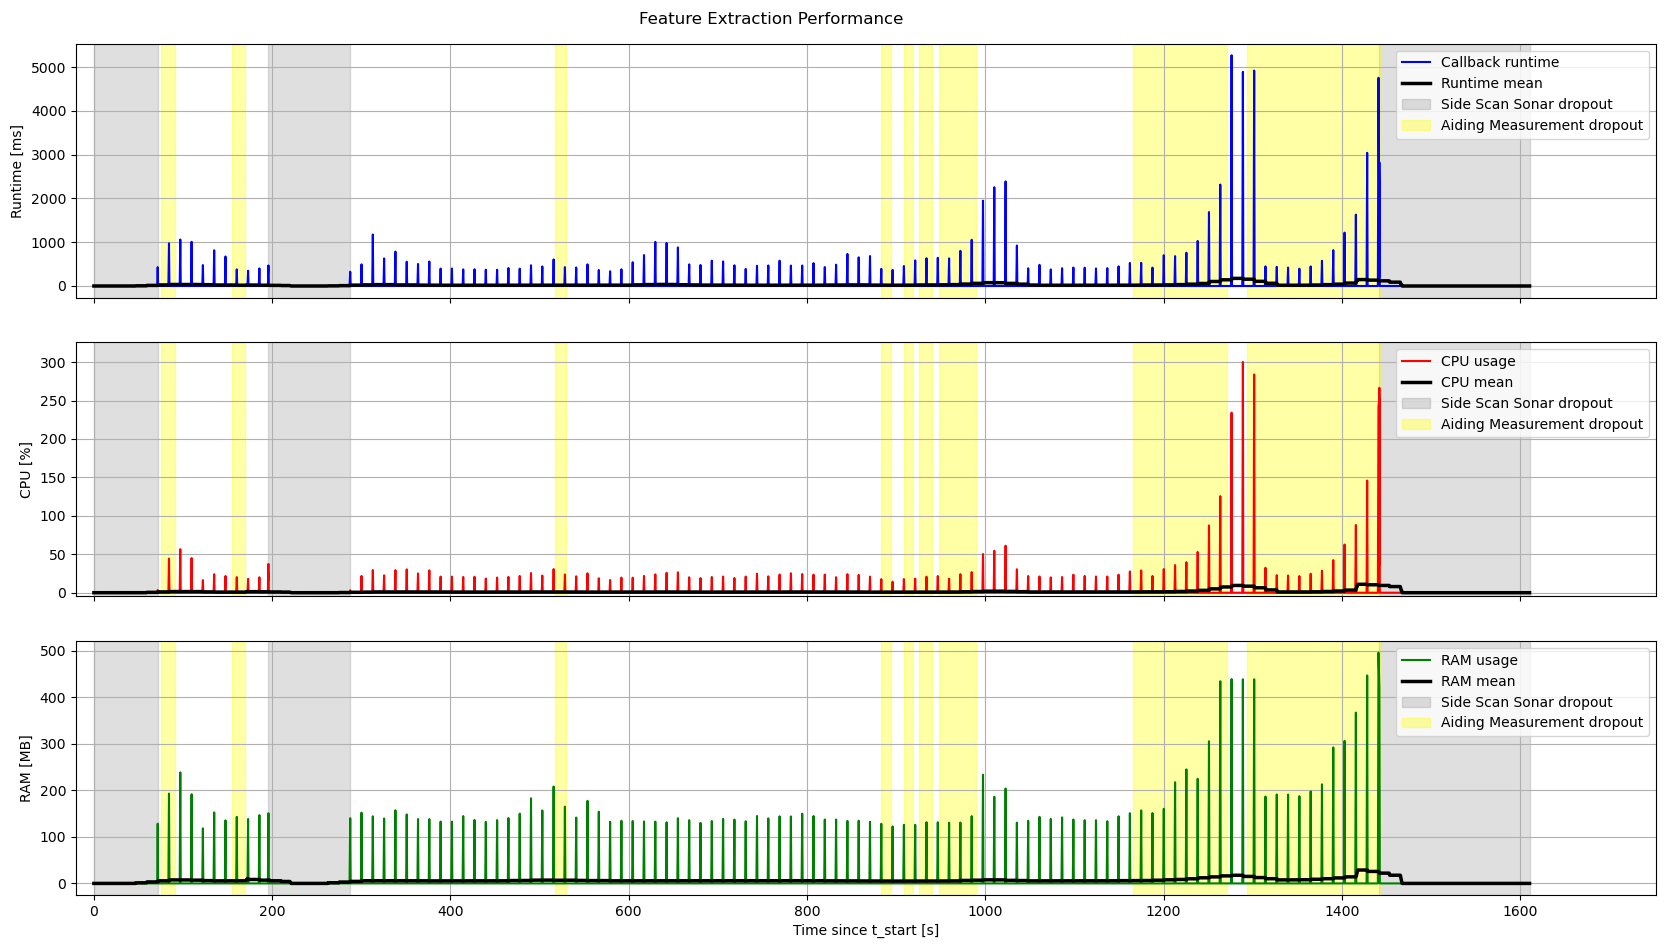
\includegraphics[width=1.00\linewidth]{Pictures/Results/Local_Map_Generation/Feature_Extraction/Performance.png}
    \caption{Runtime, CPU usage, and memory consumption of the feature extraction stage using the default parameter set.}
    \label{fig:results-local-map-generation-feature-extraction-performance}
\end{figure}
\noindent
Figure \ref{fig:results-local-map-generation-feature-extraction-performance} shows clear runtime spikes because feature extraction is only executed when a new full local map image is received. Between map updates, the node mainly waits for the next image. The runtime therefore follows the local map update rate rather than running as a continuous per swath process.
\\ \\
The peak size is mainly affected by the size of the incoming map. As discussed in the map generation results, periods with degraded aiding and increased dead reckoning drift can make the active map larger, which increases the amount of image data that must be filtered, segmented, labelled, and processed. In addition, part of the measured cost comes from transferring large image messages through the ROS2 middleware layer, not only from the feature extraction algorithm itself.
\\ \\
Profiling of the feature extraction function shows that height estimation is the most expensive internal stage, using roughly $40\%$ of the feature extraction runtime. This is expected because height estimation requires extra shadow processing for each landmark, including shadow thresholding, connected component analysis, candidate filtering, shadow length estimation, and geometric height calculation. The initial filtering stage and semantic segmentation stage each account for roughly $20\%$, while the remaining operations, including labelling, measurement generation, and descriptor construction, account for the final $20\%$.
\\ \\
To evaluate this cost, height estimation was disabled in the following run. This keeps the normal landmark detection and descriptor pipeline active, but removes the shadow based height and height uncertainty estimation.

\newpage

\begin{figure}[H]
    \centering
    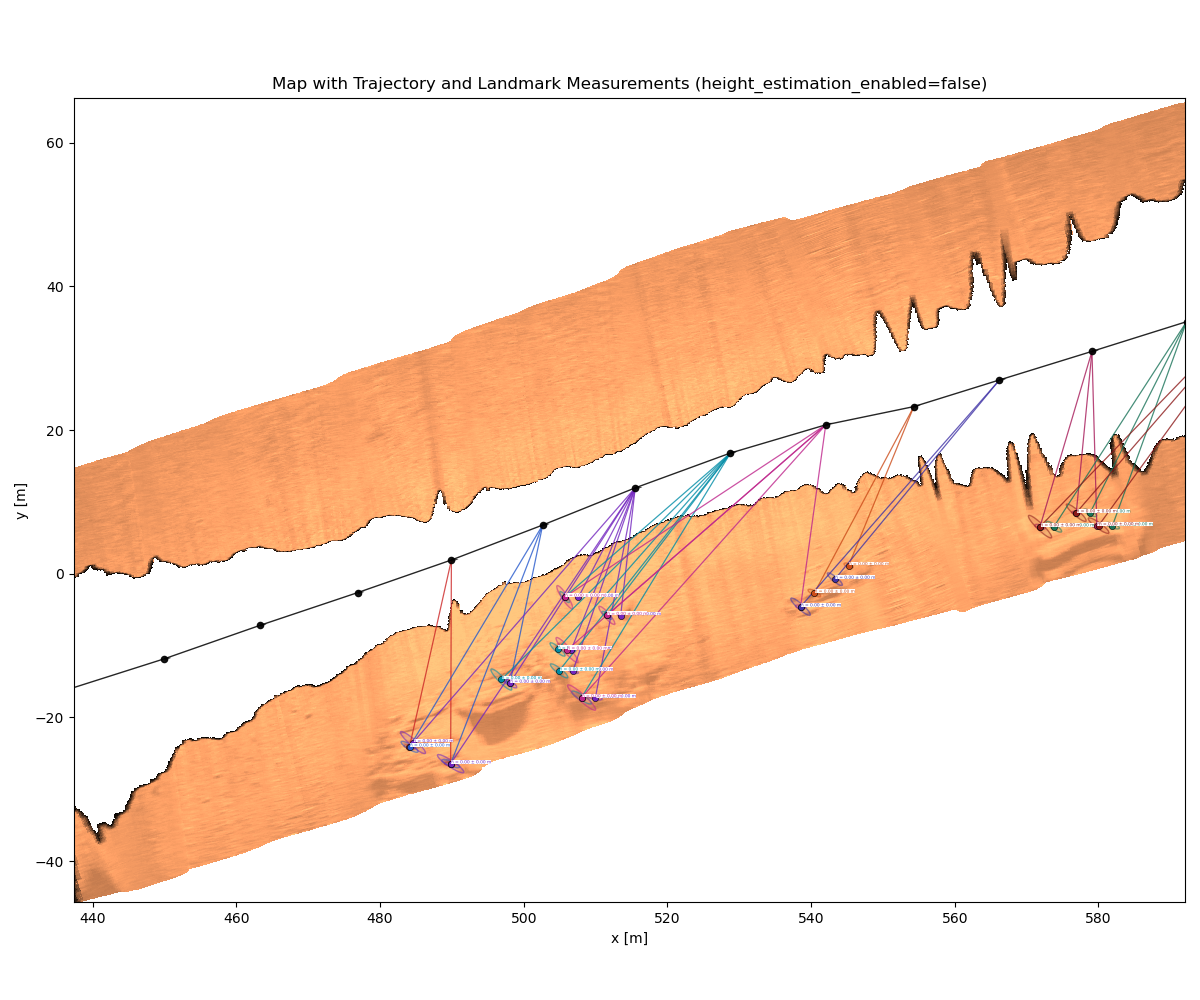
\includegraphics[width=0.70\linewidth]{Pictures/Results/Local_Map_Generation/Feature_Extraction/Full_Landmark_Measurements_NO_Height_zoomed_out.png}
    
    \vspace{0.5em}
    
    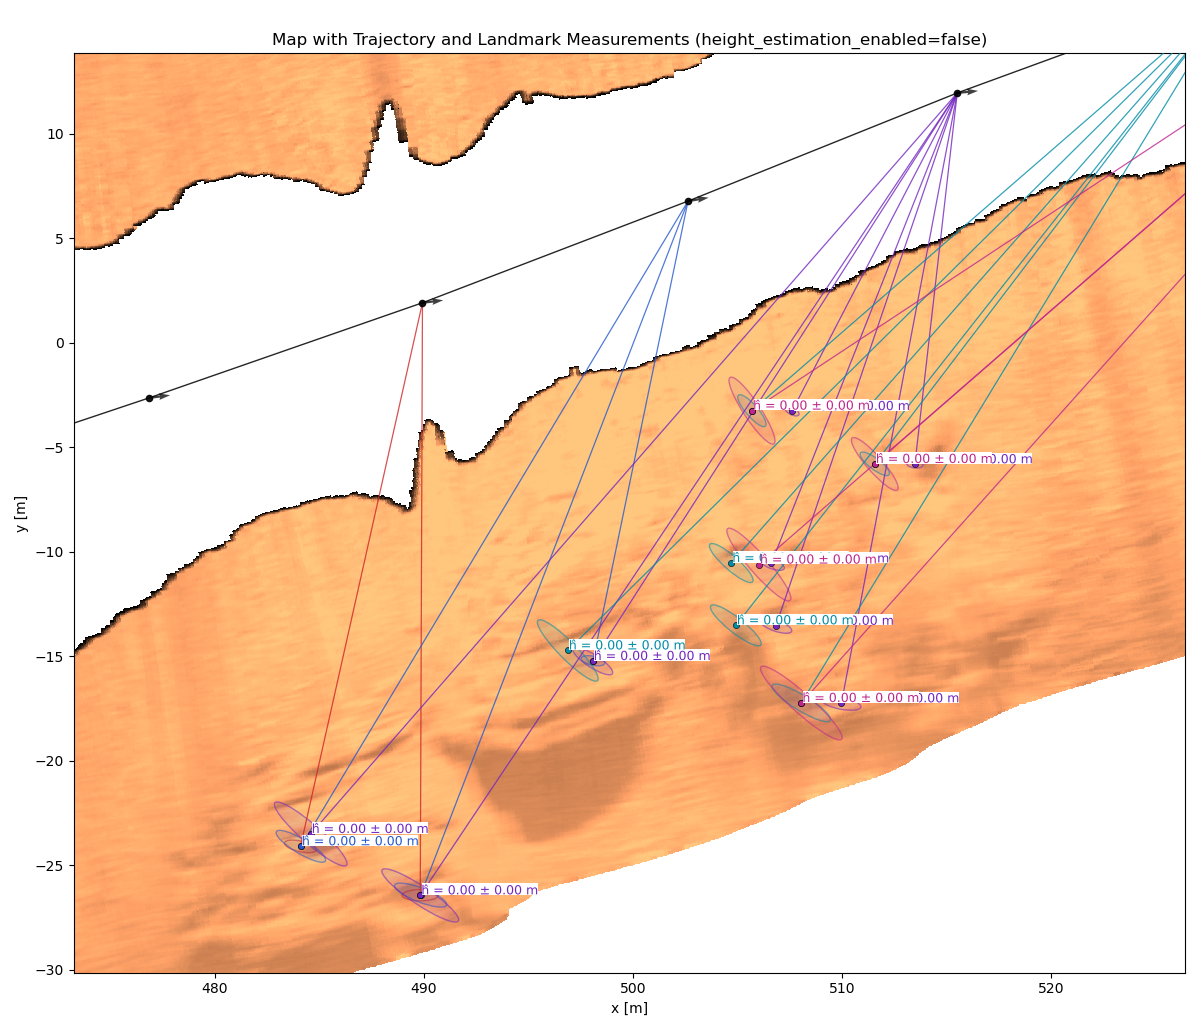
\includegraphics[width=0.70\linewidth]{Pictures/Results/Local_Map_Generation/Feature_Extraction/Full_Landmark_Measurements_NO_Height_zoomed_in.png}
    \caption{Global landmark measurements reconstructed with height estimation disabled. Landmark positions and measurements are still extracted normally, but no shadow-based height values or height uncertainties are added to the landmark output.}
    \label{fig:results-local-map-generation-feature-extraction-no-height-landmarks}
\end{figure}

\newpage

\begin{figure}[H]
    \centering
    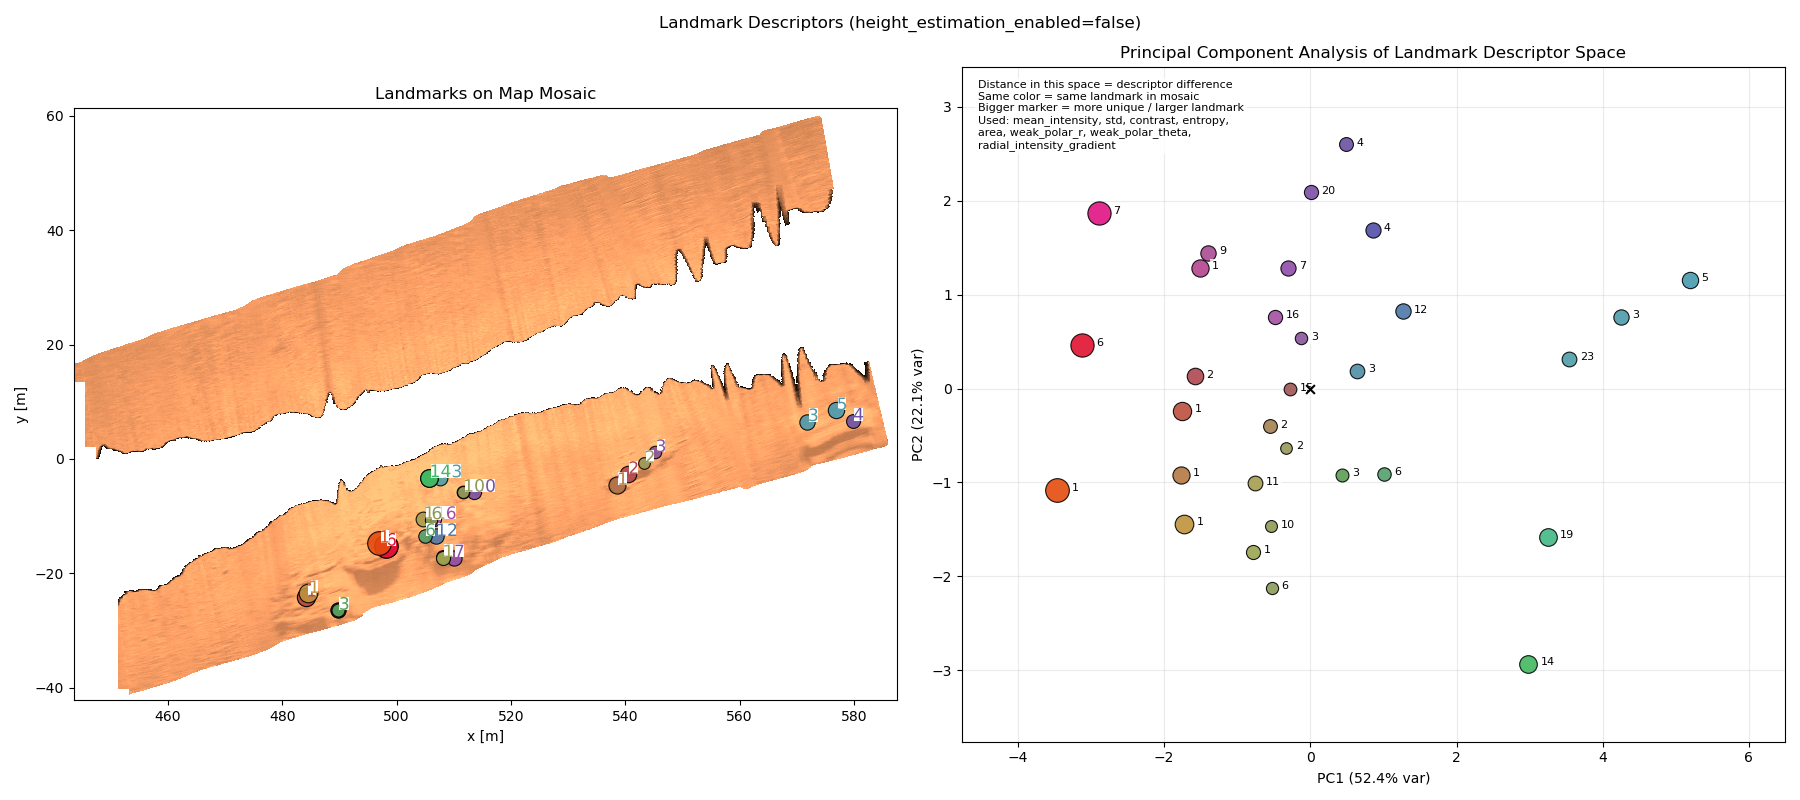
\includegraphics[width=0.95\linewidth]{Pictures/Results/Local_Map_Generation/Feature_Extraction/Full_Descriptors_NO_Height.png}
    \caption{Global landmark descriptor map with height estimation disabled. The descriptor representation still captures the remaining appearance and geometric information, but excludes the height and height uncertainty components. Since the descriptor vector changes when these components are removed, the PCA projection also changes, and the resulting descriptor colors and spatial distribution in descriptor space are not expected to match the height enabled case directly.}
    \label{fig:results-local-map-generation-feature-extraction-no-height-descriptors}
\end{figure}

\begin{figure}[H]
    \centering
    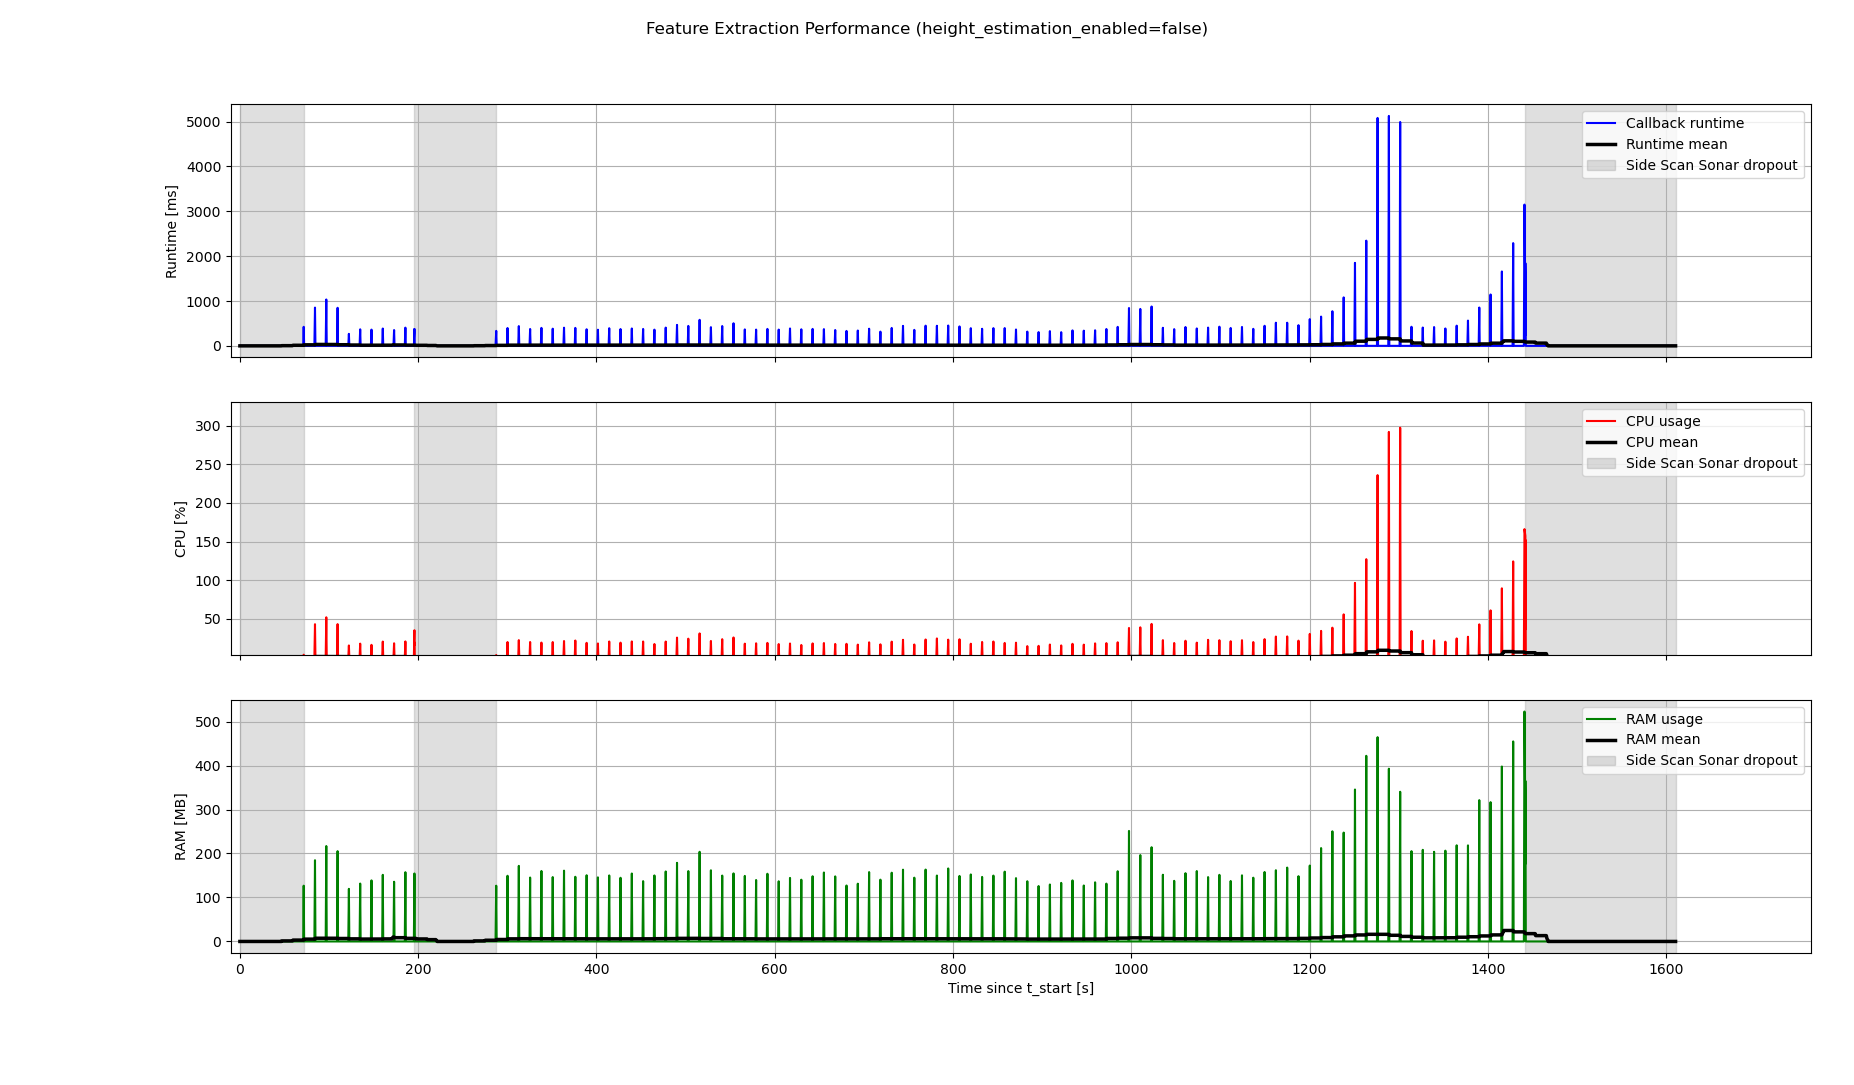
\includegraphics[width=1.00\linewidth]{Pictures/Results/Local_Map_Generation/Feature_Extraction/Performance_NO_Height.png}
    \caption{Runtime, CPU usage, and memory consumption of the feature extraction stage with height estimation disabled. The reduction is most visible during periods where landmarks are detected, since the shadow based height estimation step is skipped.}
    \label{fig:results-local-map-generation-feature-extraction-performance-no-height}
\end{figure}

\newpage

\noindent
Comparing the two performance plots shows that disabling height estimation reduces the runtime mainly in regions where landmarks are actually detected. Some peaks remain almost unchanged, because in those periods the map contains few or no valid landmark candidates, meaning the height estimation stage has little work to perform. In those cases, the runtime is dominated instead by the fixed image processing stages and by the size of the map being processed.
\\ \\
The largest differences occur during periods with several detected landmarks, especially around $300$--$350,\mathrm{s}$, $600$--$800,\mathrm{s}$, $1000$--$1050,\mathrm{s}$, and near the end of the run at approximately $1400$--$1450,\mathrm{s}$. In these regions, the full pipeline must not only filter, segment, and label the map, but also estimate shadow length and height for each detected landmark. This adds a significant extra cost, and the observed reduction is consistent with the profiling result that height estimation contributes roughly $40\%$ of the feature extraction runtime when active.
\\ \\
However, the comparison also shows that height estimation is not always the dominant system level cost. When the local map becomes large, the main cost is still the amount of image data that must be processed and moved through memory and ROS2. Therefore, reducing map size, tuning map resolution, and limiting the active map region remain the most important performance optimizations. Once the map size is controlled, disabling height estimation can provide an additional speedup if height is not required by the later SLAM or mapping stages.
